% Options for packages loaded elsewhere
\PassOptionsToPackage{unicode}{hyperref}
\PassOptionsToPackage{hyphens}{url}
\PassOptionsToPackage{dvipsnames,svgnames,x11names}{xcolor}
%
\documentclass[
  letterpaper,
  DIV=11,
  numbers=noendperiod,
  oneside]{scrreprt}
\usepackage{amsmath,amssymb}
\usepackage{lmodern}
\usepackage{iftex}
\ifPDFTeX
  \usepackage[T1]{fontenc}
  \usepackage[utf8]{inputenc}
  \usepackage{textcomp} % provide euro and other symbols
\else % if luatex or xetex
  \usepackage{unicode-math}
  \defaultfontfeatures{Scale=MatchLowercase}
  \defaultfontfeatures[\rmfamily]{Ligatures=TeX,Scale=1}
\fi
% Use upquote if available, for straight quotes in verbatim environments
\IfFileExists{upquote.sty}{\usepackage{upquote}}{}
\IfFileExists{microtype.sty}{% use microtype if available
  \usepackage[]{microtype}
  \UseMicrotypeSet[protrusion]{basicmath} % disable protrusion for tt fonts
}{}
\makeatletter
\@ifundefined{KOMAClassName}{% if non-KOMA class
  \IfFileExists{parskip.sty}{%
    \usepackage{parskip}
  }{% else
    \setlength{\parindent}{0pt}
    \setlength{\parskip}{6pt plus 2pt minus 1pt}}
}{% if KOMA class
  \KOMAoptions{parskip=half}}
\makeatother
\usepackage{xcolor}
\IfFileExists{xurl.sty}{\usepackage{xurl}}{} % add URL line breaks if available
\IfFileExists{bookmark.sty}{\usepackage{bookmark}}{\usepackage{hyperref}}
\hypersetup{
  pdftitle={MOSAIC Calculus},
  pdfauthor={Daniel Kaplan},
  colorlinks=true,
  linkcolor={blue},
  filecolor={Maroon},
  citecolor={Blue},
  urlcolor={Blue},
  pdfcreator={LaTeX via pandoc}}
\urlstyle{same} % disable monospaced font for URLs
\usepackage[left=1in,marginparwidth=2.0666666666667in,textwidth=4.1333333333333in,marginparsep=0.3in]{geometry}
\usepackage{color}
\usepackage{fancyvrb}
\newcommand{\VerbBar}{|}
\newcommand{\VERB}{\Verb[commandchars=\\\{\}]}
\DefineVerbatimEnvironment{Highlighting}{Verbatim}{commandchars=\\\{\}}
% Add ',fontsize=\small' for more characters per line
\usepackage{framed}
\definecolor{shadecolor}{RGB}{241,243,245}
\newenvironment{Shaded}{\begin{snugshade}}{\end{snugshade}}
\newcommand{\AlertTok}[1]{\textcolor[rgb]{0.68,0.00,0.00}{#1}}
\newcommand{\AnnotationTok}[1]{\textcolor[rgb]{0.37,0.37,0.37}{#1}}
\newcommand{\AttributeTok}[1]{\textcolor[rgb]{0.40,0.46,0.14}{#1}}
\newcommand{\BaseNTok}[1]{\textcolor[rgb]{0.68,0.00,0.00}{#1}}
\newcommand{\BuiltInTok}[1]{\textcolor[rgb]{0.00,0.46,0.62}{#1}}
\newcommand{\CharTok}[1]{\textcolor[rgb]{0.13,0.47,0.30}{#1}}
\newcommand{\CommentTok}[1]{\textcolor[rgb]{0.37,0.37,0.37}{#1}}
\newcommand{\CommentVarTok}[1]{\textcolor[rgb]{0.37,0.37,0.37}{\textit{#1}}}
\newcommand{\ConstantTok}[1]{\textcolor[rgb]{0.56,0.35,0.01}{#1}}
\newcommand{\ControlFlowTok}[1]{\textcolor[rgb]{0.00,0.46,0.62}{#1}}
\newcommand{\DataTypeTok}[1]{\textcolor[rgb]{0.68,0.00,0.00}{#1}}
\newcommand{\DecValTok}[1]{\textcolor[rgb]{0.68,0.00,0.00}{#1}}
\newcommand{\DocumentationTok}[1]{\textcolor[rgb]{0.37,0.37,0.37}{\textit{#1}}}
\newcommand{\ErrorTok}[1]{\textcolor[rgb]{0.68,0.00,0.00}{#1}}
\newcommand{\ExtensionTok}[1]{\textcolor[rgb]{0.00,0.46,0.62}{#1}}
\newcommand{\FloatTok}[1]{\textcolor[rgb]{0.68,0.00,0.00}{#1}}
\newcommand{\FunctionTok}[1]{\textcolor[rgb]{0.28,0.35,0.67}{#1}}
\newcommand{\ImportTok}[1]{\textcolor[rgb]{0.00,0.46,0.62}{#1}}
\newcommand{\InformationTok}[1]{\textcolor[rgb]{0.37,0.37,0.37}{#1}}
\newcommand{\KeywordTok}[1]{\textcolor[rgb]{0.00,0.46,0.62}{#1}}
\newcommand{\NormalTok}[1]{\textcolor[rgb]{0.00,0.46,0.62}{#1}}
\newcommand{\OperatorTok}[1]{\textcolor[rgb]{0.37,0.37,0.37}{#1}}
\newcommand{\OtherTok}[1]{\textcolor[rgb]{0.00,0.46,0.62}{#1}}
\newcommand{\PreprocessorTok}[1]{\textcolor[rgb]{0.68,0.00,0.00}{#1}}
\newcommand{\RegionMarkerTok}[1]{\textcolor[rgb]{0.00,0.46,0.62}{#1}}
\newcommand{\SpecialCharTok}[1]{\textcolor[rgb]{0.37,0.37,0.37}{#1}}
\newcommand{\SpecialStringTok}[1]{\textcolor[rgb]{0.13,0.47,0.30}{#1}}
\newcommand{\StringTok}[1]{\textcolor[rgb]{0.13,0.47,0.30}{#1}}
\newcommand{\VariableTok}[1]{\textcolor[rgb]{0.07,0.07,0.07}{#1}}
\newcommand{\VerbatimStringTok}[1]{\textcolor[rgb]{0.13,0.47,0.30}{#1}}
\newcommand{\WarningTok}[1]{\textcolor[rgb]{0.37,0.37,0.37}{\textit{#1}}}
\usepackage{longtable,booktabs,array}
\usepackage{calc} % for calculating minipage widths
% Correct order of tables after \paragraph or \subparagraph
\usepackage{etoolbox}
\makeatletter
\patchcmd\longtable{\par}{\if@noskipsec\mbox{}\fi\par}{}{}
\makeatother
% Allow footnotes in longtable head/foot
\IfFileExists{footnotehyper.sty}{\usepackage{footnotehyper}}{\usepackage{footnote}}
\makesavenoteenv{longtable}
\usepackage{graphicx}
\makeatletter
\def\maxwidth{\ifdim\Gin@nat@width>\linewidth\linewidth\else\Gin@nat@width\fi}
\def\maxheight{\ifdim\Gin@nat@height>\textheight\textheight\else\Gin@nat@height\fi}
\makeatother
% Scale images if necessary, so that they will not overflow the page
% margins by default, and it is still possible to overwrite the defaults
% using explicit options in \includegraphics[width, height, ...]{}
\setkeys{Gin}{width=\maxwidth,height=\maxheight,keepaspectratio}
% Set default figure placement to htbp
\makeatletter
\def\fps@figure{htbp}
\makeatother
\setlength{\emergencystretch}{3em} % prevent overfull lines
\providecommand{\tightlist}{%
  \setlength{\itemsep}{0pt}\setlength{\parskip}{0pt}}
\setcounter{secnumdepth}{5}
\usepackage{multicol}
\usepackage{afterpage}

\newenvironment{why}% 
{% 
\textcolor{blue}{\hrulefill}%
  \par\vspace{.3\baselineskip}%
  \textcolor{blue}{\scshape Why did you?}%
  \par\vspace{\baselineskip}%
}%
{\textcolor{blue}{\hrulefill}}

\newenvironment{takenote}% 
{% 
\textcolor{orange}{\hrulefill}%
  \par\vspace{.3\baselineskip}%
  \textcolor{orange}{\scshape Take note!}%
  \par\vspace{\baselineskip}%
}%
{\textcolor{orange}{\hrulefill}}

\newenvironment{practice}% 
{% 
\textcolor{olive}{\hrulefill}%
  \par\vspace{.3\baselineskip}%
  \textcolor{olive}{\scshape How it's done.}%
  \par\vspace{\baselineskip}%
}%
{\textcolor{olive}{\hrulefill}}

\newenvironment{example}% 
{% 
\textcolor{teal}{\hrulefill}%
  \par\vspace{.3\baselineskip}%
  \textcolor{teal}{\scshape For instance ...}%
  \par\vspace{\baselineskip}%
}%
{\textcolor{teal}{\hrulefill}}


\newenvironment{intheworld}% 
{% 
\textcolor{magenta}{\hrulefill}%
  \par\vspace{.3\baselineskip}%
  \textcolor{magenta}{\scshape Math in the world ...}%
  \par\vspace{\baselineskip}%
}%
{\textcolor{magenta}{\hrulefill}}

\newenvironment{scaffolding}% 
{% 
\textcolor{brown}{\hrulefill}%
  \par\vspace{.3\baselineskip}%
  \textcolor{brown}{\scshape Open an R console and ....}%
  \par\vspace{\baselineskip}%
}%
{\textcolor{brown}{\hrulefill}}

\newenvironment{rmosaic}% 
{% 
\textcolor{brown}{\hrulefill}%
  \par\vspace{.3\baselineskip}%
  \textcolor{brown}{\scshape R/mosaic commands}%
  \par\vspace{\baselineskip}%
}%
{\textcolor{brown}{\hrulefill}}

\newenvironment{madeeasy}% 
{% 
\textcolor{orange}{\hrulefill}%
  \par\vspace{.3\baselineskip}%
  \textcolor{orange}{\scshape Calculus Made Easy}%
  \par\vspace{\baselineskip}%
}%
{\textcolor{orange}{\hrulefill}}


\newenvironment{tip}% 
{% 
\textcolor{teal}{\hrulefill}%
  \par\vspace{.3\baselineskip}%
  \textcolor{teal}{\scshape A Tip!}%
  \par\vspace{\baselineskip}%
}%
{\textcolor{teal}{\hrulefill}}

\newenvironment{underconstruction}% 
{% 
\textcolor{teal}{\hrulefill}%
  \par\vspace{.3\baselineskip}%
  \textcolor{teal}{\scshape UNDER CONSTRUCTION!}%
  \par\vspace{\baselineskip}%
}%
{\textcolor{teal}{\hrulefill}}

\renewcommand{\line}{\text{line}}
\newcommand{\hump}{\text{hump}}
\newcommand{\sigmoid}{\text{sigmoid}}
\newcommand{\recip}{\text{recip}}
\newcommand{\diff}[1]{{\cal D}_#1}
\newcommand{\pnorm}{\text{pnorm}}
\newcommand{\dnorm}{\text{dnorm}}
\let\origvec\vec
\let\origmathit\mathit
\let\orighat\hat
\let\origbar\bar
\renewcommand{\vec}[1]{\overset{{\rule[-1pt]{0mm}{1mm}}\rightharpoonup}{\mathbf{#1}}}
\renewcommand{\bar}[1]{\overset{{\rule[-1pt]{12pt}{.5mm}}}{\mathbf{#1}}}
\renewcommand{\mathit}[1]{\underset{\leftharpoondown}{\overset{{\rightharpoonup}}{\large\mathbf #1}}}
\renewcommand{\hat}[1]{\widehat{\ \mathbf#1\ }}
\newcommand{\len}[1]{{\|{\mathbf #1}\|}}
\newcommand{\tvec}[1]{\overset{\uparrow}{\mathbf #1}}
\newcommand{\tmat}[1]{\overset{\leftrightarrows}{\mathbf #1}}
\newcommand{\perpendicularto}[2]{#1\!\perp\!#2}
\newcommand{\modeledby}[2]{#1\!\sim\!#2}
\newcommand{\CC}[1]{\color{\#648fff}{#1}}
\newcommand{\CE}[1]{\color{\#785ef0}{#1}}
\newcommand{\CA}[1]{\color{\#dc267f}{#1}}
\newcommand{\CB}[1]{\color{\#fe6100}{#1}}
\newcommand{\CD}[1]{\color{\#ffb000}{#1}}
\newcommand{\bcancel}[1]{XX{#1}}
\newcommand{\cancel}[1]{X{#1}X}
\usepackage{booktabs}
\usepackage{longtable}
\usepackage{array}
\usepackage{multirow}
\usepackage{wrapfig}
\usepackage{float}
\usepackage{colortbl}
\usepackage{pdflscape}
\usepackage{tabu}
\usepackage{threeparttable}
\usepackage{threeparttablex}
\usepackage[normalem]{ulem}
\usepackage{makecell}
\usepackage{xcolor}
\KOMAoption{captions}{tableheading}
\makeatletter
\makeatother
\makeatletter
\@ifpackageloaded{caption}{}{\usepackage{caption}}
\AtBeginDocument{%
\renewcommand*\contentsname{Table of contents}
\renewcommand*\listfigurename{List of Figures}
\renewcommand*\listtablename{List of Tables}
\renewcommand*\figurename{Figure}
\renewcommand*\tablename{Table}
}
\@ifpackageloaded{float}{}{\usepackage{float}}
\floatstyle{ruled}
\@ifundefined{c@chapter}{\newfloat{codelisting}{h}{lop}}{\newfloat{codelisting}{h}{lop}[chapter]}
\floatname{codelisting}{Listing}
\newcommand*\listoflistings{\listof{codelisting}{List of Listings}}
\makeatother
\makeatletter
\@ifpackageloaded{caption}{}{\usepackage{caption}}
\@ifpackageloaded{subcaption}{}{\usepackage{subcaption}}
\makeatother
\makeatletter
\@ifpackageloaded{sidenotes}{}{\usepackage{sidenotes}}
\@ifpackageloaded{marginnote}{}{\usepackage{marginnote}}
\makeatother
\makeatletter
\@ifpackageloaded{tcolorbox}{}{\usepackage[many]{tcolorbox}}
\makeatother
\makeatletter
\@ifundefined{shadecolor}{\definecolor{shadecolor}{rgb}{.97, .97, .97}}
\makeatother
\makeatletter
\makeatother
\ifLuaTeX
  \usepackage{selnolig}  % disable illegal ligatures
\fi

\title{MOSAIC Calculus}
\author{Daniel Kaplan}
\date{4/18/2022}

\begin{document}
\maketitle

\ifdefined\Shaded\renewenvironment{Shaded}{\begin{tcolorbox}[interior hidden, enhanced, borderline west={3pt}{0pt}{shadecolor}, frame hidden, boxrule=0pt, sharp corners]}{\end{tcolorbox}}\fi

\renewcommand*\contentsname{Table of contents}
{
\hypersetup{linkcolor=}
\setcounter{tocdepth}{2}
\tableofcontents
}
\hypertarget{preface}{%
\chapter*{Preface}\label{preface}}
\addcontentsline{toc}{chapter}{Preface}

\hypertarget{tips-in-draft}{%
\section*{Tips in draft}\label{tips-in-draft}}
\addcontentsline{toc}{section}{Tips in draft}

\texttt{GIT\_TRACE=1\ git\ push}

or

\texttt{git\ push\ -\/-force\ origin\ main}

\hypertarget{acknowledements}{%
\section*{Acknowledements}\label{acknowledements}}
\addcontentsline{toc}{section}{Acknowledements}

This project was initiated by the Mathematical Sciences department at
the US Air Force Academy. They recognized that a traditional calculus
introduction is ill-suited to the needs of STEM in the 21st century.

Critical support was given by the \href{http://ardifoundation.org}{ARDI
Foundation} which awarded the
\href{http://www.ardifoundation.org/coors-chair/}{Holland H. Coors Chair
in Education Technology} to one of the project members, Daniel Kaplan.
This made possible a year-long residency at USAFA during which time he
was able to work unhindered on this project.

Macalester College, where Kaplan is DeWitt Wallace Professor of
Mathematics, Statistics, and Computer science, was the site where the
overall framework and many of the materials for a STEM-oriented calculus
were developed. Particularly important in the germination were David
Bressoud and Jan Serie, respectively chairs of the Macalester math and
biology departments, as well as Prof.~Thomas Halverson and Prof.~Karen
Saxe, who volunteered to team teach with Kaplan the first prototype
course. Early grant support from the Howard Hughes Medical Foundation
and the Keck Foundation provided the resources to carry the prototype
course to a point of development where it became the entryway to
calculus for Macalester students.

Profs. Randall Pruim (Calvin University) and Nicholas Horton (Amherst
College) were essential collaborators in developing software to support
calculus in R. They and Kaplan formed the core team of Project MOSAIC,
which was supported by the US National Science Foundation (NSF
DUE-0920350).

Joel Kilty and Alex McAllister at Centre College admired the Macalester
course and devoted much work and ingenuity to write a textbook,
\emph{Mathematical Modeling and Applied Calculus} (Oxford Univ. Press),
implementing their own version. Their textbook enabled us to reduce the
use of sketchy notes in the first offering of this course at USAFA.

\part{Accumulation}

This is where I'll explain what the block is about and the overall
goals.

\hypertarget{sec-change-accumulation}{%
\chapter{Change \& accumulation}\label{sec-change-accumulation}}

Every 10 years, starting in 1790, the US Census Bureau carries out a
constitutionally mandated census: a count of the current population. The
overall count as a function of year is shown in
Figure~\ref{fig-pop-graph}.
{[}\href{https://en.wikipedia.org/wiki/Demographic_history_of_the_United_States}{Source}{]}

In the 230 years spanned by the census data, the US population has grown
100-fold, from about 4 million in 1790 to about 330,000,000 in 2020.

\begin{figure}

\sidecaption{\label{fig-pop-graph}US population since 1790. Left: linear
axes. Right: semi-log axes}

{\centering 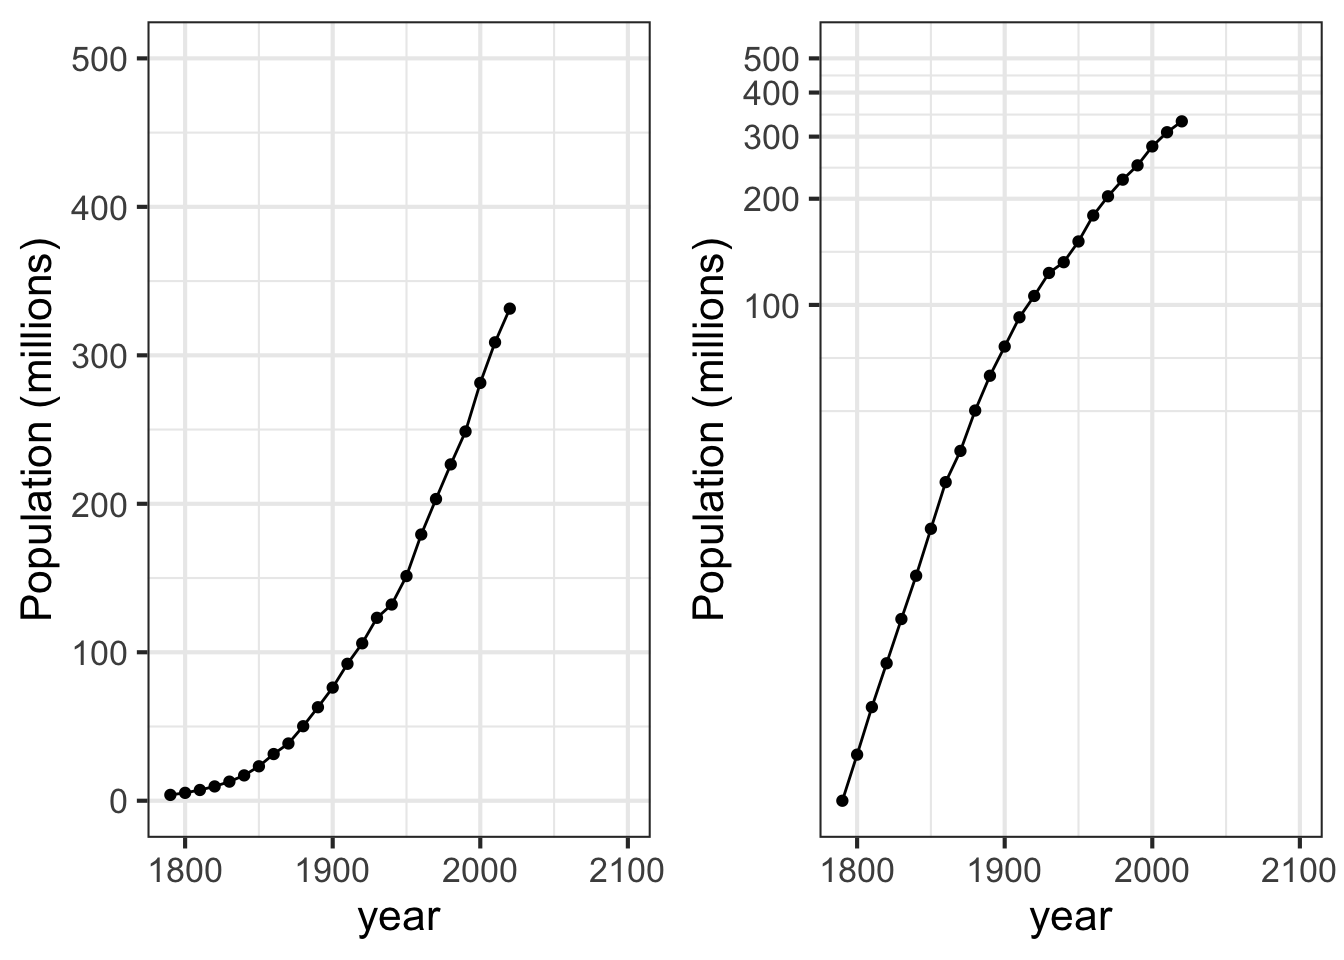
\includegraphics[width=0.9\textwidth,height=\textheight]{Accumulation/27-intro_files/figure-pdf/fig-pop-graph-1.pdf}

}

\end{figure}

It's tempting to look for simple patterns in such data. Perhaps the US
population has been growing exponentially. A semi-log plot of the same
data suggests that the growth is only very roughly exponential. A truly
exponential process would present as a curve with a constant derivative,
but the derivative of the function in the graph is decreasing over the
centuries.

Insofar as the slope over the semi-log graph is informative, it amounts
to this quantity:
\[\partial_t \ln(\text{pop}(t)) = \frac{\partial_t\, \text{pop}(t)}{\text{pop}}\]
This is the \emph{per-capita} rate of growth, that is, the rate of
change in the population divided by the population. Conventionally, this
fraction is presented as a percentage: percentage growth in the
population per year, as in Figure~\ref{fig-pop-growth}.

\begin{figure}

\sidecaption{\label{fig-pop-growth}Annual per capita growth rate of the
US population (percent)}

{\centering 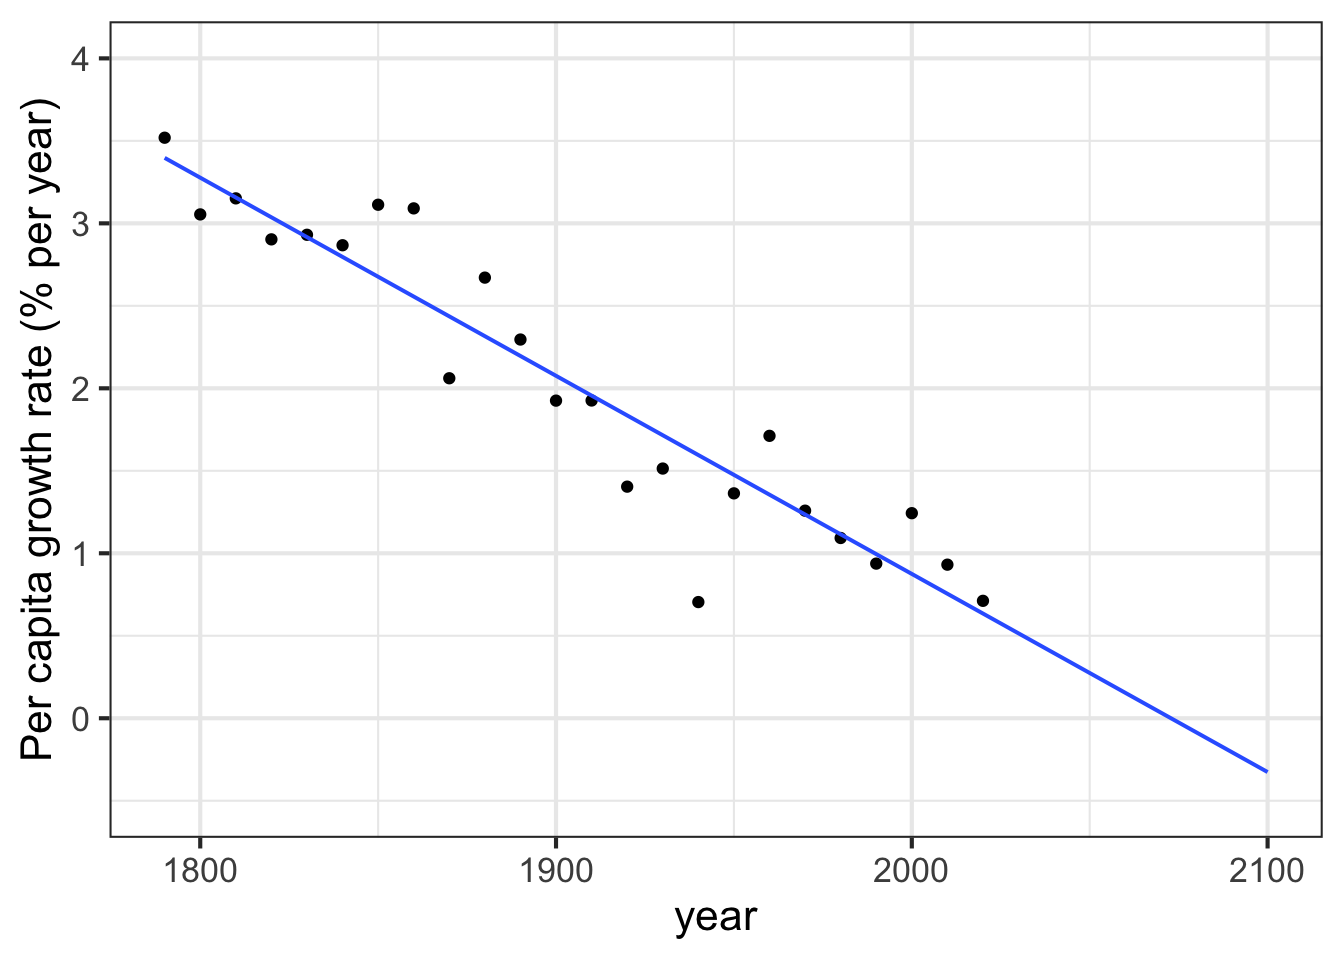
\includegraphics[width=0.9\textwidth,height=\textheight]{Accumulation/27-intro_files/figure-pdf/fig-pop-growth-1.pdf}

}

\end{figure}

The dots in the graph are a direct calculation from the census data.
There's a lot of fluctuation, but an overall trend stands out: the
population growth rate has been declining since the mid-to late 1800s.
The deviations from the trend are telling and correspond to historical
events. There's a relatively low growth rate seen from 1860 to 1870:
that's the effect of the US Civil War. The Great depression is seen in
the very low growth from 1930 to 1940. Baby Boom: look at the growth
from 1950-1960. The bump from 1990 to 2000? Not coincidentally, the 1990
Immigration Act substantially increased the yearly rate of immigration.

If the trend in the growth rate continues, the US will reach zero net
growth about 2070, then continue with negative growth. Of course,
negative growth is just decline. A simple prediction from
Figure~\ref{fig-pop-growth} is that the argmax of the US
population---that is, the year that the growth rate reaches zero---will
occur around 2070.

How large will the population be when it reaches its maximum?

In Block 2, we dealt with situations where we know the function \(f(t)\)
and want to find the rate of change \(\partial_t f(t)\). Here, we know
the rate of change of the population and we need to figure out the
population itself, in other words to figure out from a known
\(\partial_t f(t)\) what is the unknown function \(f(t)\).

The process of figuring out \(f(t) \longrightarrow \partial_t f(t)\) is,
of course, called \textbf{\emph{differentiation}}. The opposite process,
\(\partial_t f(t) \longrightarrow f(t)\) is called
\textbf{\emph{anti-differentiation}}.

In this block we'll explore the methods for calculating anti-derivatives
and some of the settings in which anti-derivative problems arrive.

\begin{intheworld}
The predictions from the accumulate-population-growth model are shown as
a \(\color{magenta}{\text{magenta}}\) line in
Figure~\ref{fig-pop-prediction-bad}.

\begin{figure}

{\centering 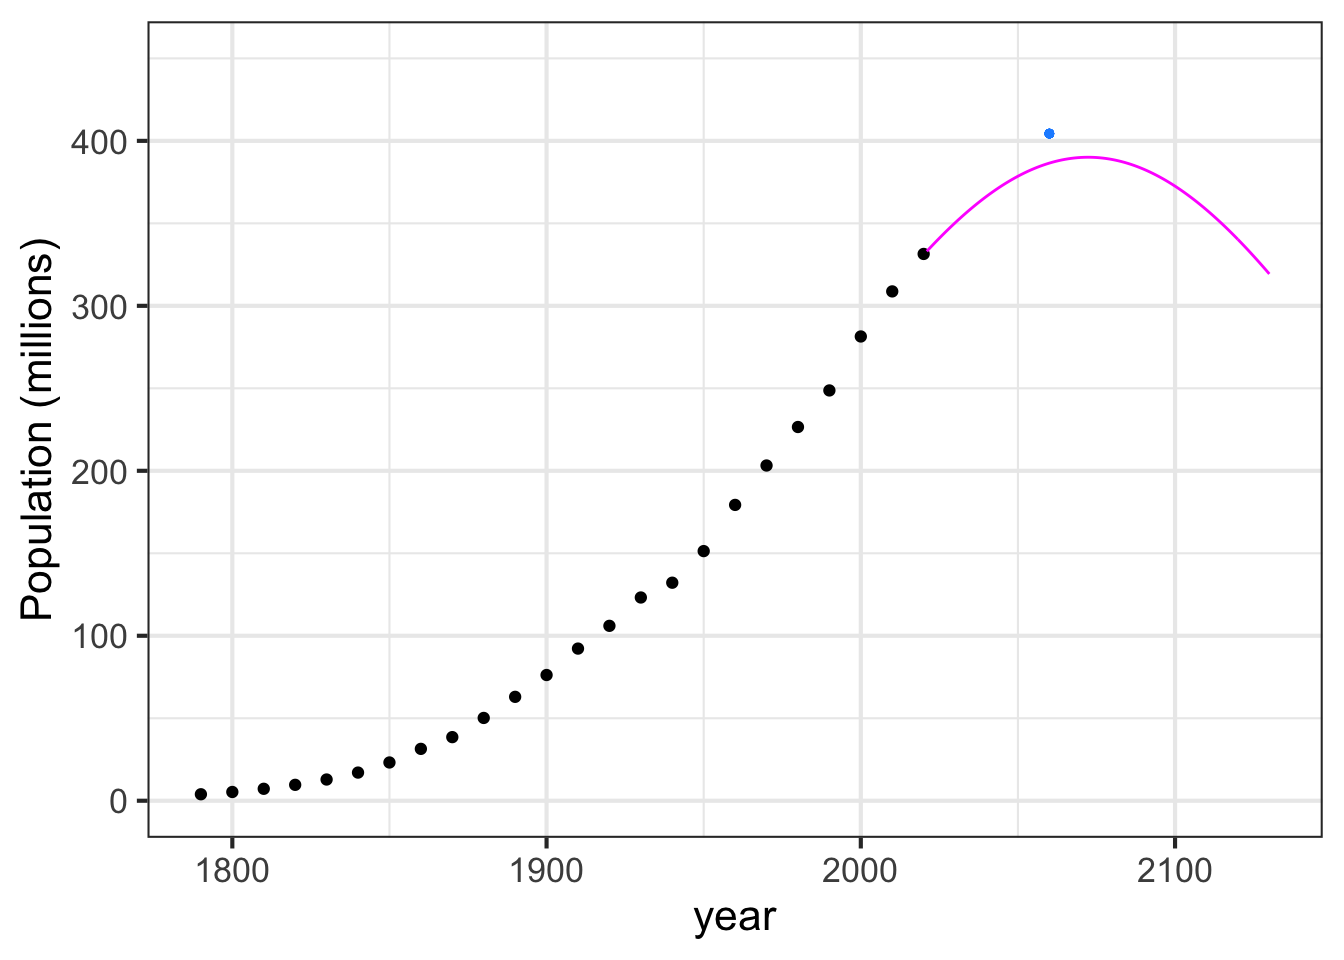
\includegraphics[width=0.9\textwidth,height=\textheight]{Accumulation/27-intro_files/figure-pdf/fig-pop-prediction-bad-1.pdf}

}

\caption{\label{fig-pop-prediction-bad}Predicted US population based on
the historical linear decline in per-capita growth.}

\end{figure}

According to the accumulation model, the population peaks in 2075 at 390
million. We'll be back down to the present population level in about 100
years.

Professional demographers make much more sophisticated models using
detailed data from many sources. The demographers at the US Census
Bureau predict that the population will reach a maximum of 404 million
in 2060, shown by the little blue dot in
Figure~\ref{fig-pop-prediction-bad}. That's not too different from what
we got by analyzing just the raw census numbers.

\end{intheworld}

\hypertarget{accumulation}{%
\section{Accumulation}\label{accumulation}}

Imagine a simple setting: water flowing out of a tap into a basin or
tank. The amount of water in the basin will be measured in a unit of
volume, say liters. Measurement of the \emph{flow} \(f(t)\) of water
from the tap into the tank has different units, say liters per second.
If volume \(V(t)\) is the volume of water in the tank as a function of
time, \(f(t)\) at any instant is \(f(t) = \partial_t V(t)\).

Clearly there is a relationship between the two functions \(f(t)\) and
\(V(t)\). With derivatives, we can give a good description of that
relationship: \[f(t) = \partial_t V(t)\] This description will be
informative if we have measured the volume of water in the basin as a
function of time and want to deduce the rate of flow from the tap. Now
suppose we have measured the flow \(f(t)\) and want to figure out the
volume. The volume at any instant is the past flow accumulated to that
instant. As a matter of notation, we write this view of the relationship
as \[V(t) = \int f(t) dt,\] which you can read as ``volume is the
accumulated flow.''

Other examples of accumulation and change:

\begin{itemize}
\tightlist
\item
  velocity is the rate of change of position \emph{with respect to
  time}. Likewise, position is the accumulation of velocity \emph{over
  time}.
\item
  force is the rate of energy \emph{with respect to position}. Likewise
  energy is the accumulation of force \emph{as position changes}.
\item
  deficit is the rate of change of debt with respect to time. Likewise,
  debt is the accumulation of deficit over time.
\end{itemize}

\hypertarget{notation-for-anti-differentiation}{%
\section{Notation for
anti-differentiation}\label{notation-for-anti-differentiation}}

For differentiation we are using the notation \(\partial_x\) as in
\(\partial_x f(x)\). Remember that the subscript on \(\partial\) names
the \textbf{\emph{with-respect-to input}}. There are three pieces of
information this notation:

\begin{enumerate}
\def\labelenumi{\arabic{enumi}.}
\tightlist
\item
  The \(\color{magenta}{\partial}\) symbol which identifies the
  operation as partial \textbf{\emph{differentiation}}.
\item
  The name of the with-respect-to input
  \(\partial_{\color{magenta}{x}}\) written as a subscript to
  \(\partial\).
\item
  The function to be differentiated,
  \(\partial_x \color{magenta}{f(x)}\).
\end{enumerate}

For \textbf{\emph{anti-differentiation}}, our notation must also specify
the three pieces of information. It might be tempting to use the same
notation as differentiation but replace the \(\partial\) symbol with
something else, perhaps \(\eth\) or \(\spadesuit\) or \(\forall\),
giving us something like \(\spadesuit_x f(x)\).

Convention has something different in store. The notation for
anti-differentiation is \[\large \int f(x) dx\] 1. The
\(\color{magenta}{\int}\) is the marker for anti-differentiation. 2. The
name of the with-respect-to input is contained in the ``dx'' at the end
of the notation: \(\int f(x) d\color{magenta}{x}\) 3. The function being
anti-differentiated is in the middle \(\int \color{magenta}{f(x)} dx\).

For those starting out with anti-differentiation, the conventional
notation can be confusing, especially the \(dx\) part. It's easy confuse
\(d\) for a constant and \(x\) for part of the function being
anti-differentiated.

Think of the \(\int\) and the \(dx\) as \textbf{brackets} around the
function. You need both brackets for correct notation, the \(\int\) and
the \(dx\) together telling you what operation to perform.

Remember that just as \(\partial_x f(x)\) is a function, so is
\(\int f(x) dx\).

\hypertarget{rmosaic-notation}{%
\section{R/mosaic notation}\label{rmosaic-notation}}

Recall that the notation for differentiation in R/mosaic is
\texttt{D(f(x)\ \textasciitilde{}\ x)}. The R/mosaic notation for
anti-differentiation is very similar:

\begin{Shaded}
\begin{Highlighting}[]
\FunctionTok{D}\NormalTok{(}\FunctionTok{f}\NormalTok{(x) }\SpecialCharTok{\textasciitilde{}}\NormalTok{ x)}
\end{Highlighting}
\end{Shaded}

This has the same three pieces of information as \(\partial_x f(x)\)

\begin{enumerate}
\def\labelenumi{\arabic{enumi}.}
\tightlist
\item
  \texttt{D()} signifies differentiation whereas \texttt{antiD()}
  signifies anti-differentiation.
\item
  \texttt{\textasciitilde{}\ x} identifies the with-respect-to input.
\item
  \texttt{f(x)\ \textasciitilde{}} is the function on which the
  operation is to be performed.
\end{enumerate}

Remember that just as \texttt{D(f(x)\ \textasciitilde{}\ x)} creates a
new function out of \texttt{f(x)\ \textasciitilde{}\ x}, so does
\texttt{antiD(f(x)\ \textasciitilde{}\ x)}.

\hypertarget{dimension-and-anti-differentiation}{%
\section{Dimension and
anti-differentiation}\label{dimension-and-anti-differentiation}}

This entire block will be about anti-differentiation, its properties and
its uses. You already know that anti-differentiation (as the name
suggests) is the inverse of differentiation. There is one consequence of
this that is helpful to keep in mind as we move on to other chapters.
This being calculus, the functions that we construct and operate upon
have inputs that are quantities and outputs that are also quantities.
Every quantity has a dimension, as discussed in Chapter 16. When you are
working with any quantity, you should be sure that you know its
dimension and its units.

The dimension of the input to a function does not by any means have to
be the same as the dimension of the output. For instance, we have been
using many functions where the input has dimension \textbf{time} and the
output is position (dimension L) or velocity (dimension L/T) or
acceleration (dimension L/T\(^2\)).

Imagine working with some function \(f(y)\) that's relevant to some
modeling project of interest to you. Returning to the bracket notation
that we used in Chapter 16, the dimension of the input quantity will be
{[}\(y\){]}. The dimension of the output quantity is {[}\(f(y)\){]}.
(Remember from 16 that {[}\(y\){]} means ``the dimension of quantity
\(y\)'' and that {[}\(f(y)\){]} means ``the dimension of the
\emph{output} from \(f(y)\).'')

The function \(\partial_y f(y)\) has the same input dimension \([y]\)
but the output will be \([f(y)] / [y]\). For example, suppose \(f(y)\)
is the mass of fuel in a rocket as a function of time \(y\). The output
of \(f(y)\) has dimension M. The input dimension \([y]\) is T.

The output of the function \(\partial_y f(y)\) has dimension
\([f(y)] / [y]\), which in this case will be M / T. (Less abstractly, if
the fuel mass is given in kg, and time is measured in seconds, then
\(\partial_y f(y)\) will have units of kg-per-second.)

How about the dimension of the anti-derivative \(F(y) = \int f(y) dy\)?
Since \(F(y)\) is the anti-derivative of \(f(y)\) (with respect to
\(y\)), we know that \(\partial_y F(y) = f(y)\). Taking the dimension of
both sides
\[[\partial_y F(y)] = \frac{[F(y)]}{[y]} = \frac{[F(y)]}{\text{T}} = [f(y)] = \text{M}\]
Consequently, \([F(y)] = \text{M}\).

To summarize:

\begin{itemize}
\tightlist
\item
  The dimension of derivative \(\partial_y f(y)\) will be
  \([f(y)] / [y]\).
\item
  The dimension of the anti-derivative \(\int f(y) dy\) will be
  \([f(y)]\times [y]\).
\end{itemize}

Or, more concisely:

\begin{quote}
Differentiation is like division, anti-differentiation is like
multiplication.
\end{quote}

Paying attention to the dimensions (and units!) of input and output can
be a boon to the calculus student. Often students have some function
\(f(y)\) and they are wondering which of the several calculus operations
they are supposed to do: differentiation, anti-differentiation, finding
a maximum, finding an argmax or a zero. Start by figuring out the
dimension of the quantity you want. From that, you can often figure out
which operation is appropriate.

To illustrate, imagine that you have constructed \(f(y)\) for your task
and you know, say,
\[[f(y)] = \text{M       and} \  \ \ \ \ [y] = \text{T}\ .\] Look things
up in the following table:

\begin{longtable}[]{@{}ll@{}}
\toprule
Dimension of result & Calculus operation \\
\midrule
\endhead
M / T & differentiate \\
M T & anti-differentiate \\
M & find max or min \\
T & find argmax/argmin or a function zero \\
M T\(^2\) & anti-differentiate twice in succession \\
M / T\(^2\) & differentiate twice in succession \\
\bottomrule
\end{longtable}

For example, suppose the output of the accelerometer on your rocket has
dimension L / T\(^2\). You are trying to figure out from the
accelerometer reading what is your altitude. Altitude has dimension L.
Look up in the table to see that you want to anti-differentiate
acceleration twice in succession.

\hypertarget{sec-preliminary-terrors}{%
\section{\texorpdfstring{From \emph{Calculus Made
Easy}}{From Calculus Made Easy}}\label{sec-preliminary-terrors}}

\href{https://en.wikipedia.org/wiki/Calculus_Made_Easy}{\emph{Calculus
Made Easy}}, by Silvanus P. Thompson, is a classic, concise, and elegant
textbook from 1910. It takes a common-sense approach, sometimes
lampooning the traditional approach to teaching calculus.

\begin{quote}
\emph{Some calculus-tricks are quite easy. Some are enormously
difficult. The fools who write the textbooks of advanced
mathematics---and they are mostly clever fools---seldom take the trouble
to show you how easy the easy calculations are. On the contrary, they
seem to desire to impress you with their tremendous cleverness by going
about it in the most difficult way.} --- From the preface
\end{quote}

Thompson's first chapter starts with the notation of accumulation, which
he calls ``the preliminary terror.''

\begin{madeeasy}
The preliminary terror \ldots{} can be abolished once for all by simply
stating what is the meaning---in common-sense terms---of the two
principal symbols that are used in calculating.

These dreadful symbols are:

\begin{enumerate}
\def\labelenumi{(\arabic{enumi})}
\tightlist
\item
  \(\Large\  d\) which merely means ``a little bit of.''
\end{enumerate}

Thus \(dx\) means a little bit of \(x\); or \(du\) means a little bit of
\(u\). Ordinary mathematicians think it more polite to say ``an element
of,'' instead of ``a little bit of.'' Just as you please. But you will
find that these little bits (or elements) may be considered to be
indefinitely small.

\begin{enumerate}
\def\labelenumi{(\arabic{enumi})}
\setcounter{enumi}{1}
\tightlist
\item
  \(\ \ \large\int\) which is merely a long \(S\), and may be called (if
  you like) ``the sum of.''
\end{enumerate}

Thus \(\ \int dx\) means the sum of all the little bits of \(x\); or
\(\ \int dt\) means the sum of all the little bits of \(t\). Ordinary
mathematicians call this symbol ``the integral of.'' Now any fool can
see that if \(x\) is considered as made up of a lot of little bits, each
of which is called \(dx\), if you add them all up together you get the
sum of all the \(dx\)'s, (which is the same thing as the whole of
\(x\)). The word ``integral'' simply means ``the whole.'' If you think
of the duration of time for one hour, you may (if you like) think of it
as cut up into \(3600\) little bits called seconds. The whole of the
\(3600\) little bits added up together make one hour.

When you see an expression that begins with this terrifying symbol, you
will henceforth know that it is put there merely to give you
instructions that you are now to perform the operation (if you can) of
totaling up all the little bits that are indicated by the symbols that
follow.

\end{madeeasy}

\begin{center}\rule{0.5\linewidth}{0.5pt}\end{center}

The next chapter shows what it means to ``total up all the little bits''
of a function.

\hypertarget{exercises}{%
\section{Exercises}\label{exercises}}

\hypertarget{sec-totaling-bits}{%
\chapter{Totaling the little bits}\label{sec-totaling-bits}}

Many students wonder how it is possible to reconstruct a function
\(F(x)\) from its derivative \(f(x)\). The point of this short chapter
is to help you develop some intuition about anti-differentiation.

You already know the notation meaning ``\(F(x)\) is the anti-derivative
of \(f(x)\)'': \[\large \int f(x)\, dx\ .\] In drawing a graph of
\(F(x)\), we will of course want to use coordinate axes where the
quantity \(x\) is represented on the horizontal axis and the quantity of
the output \(F(x)\) is on the vertical axis:

\begin{figure}

{\centering 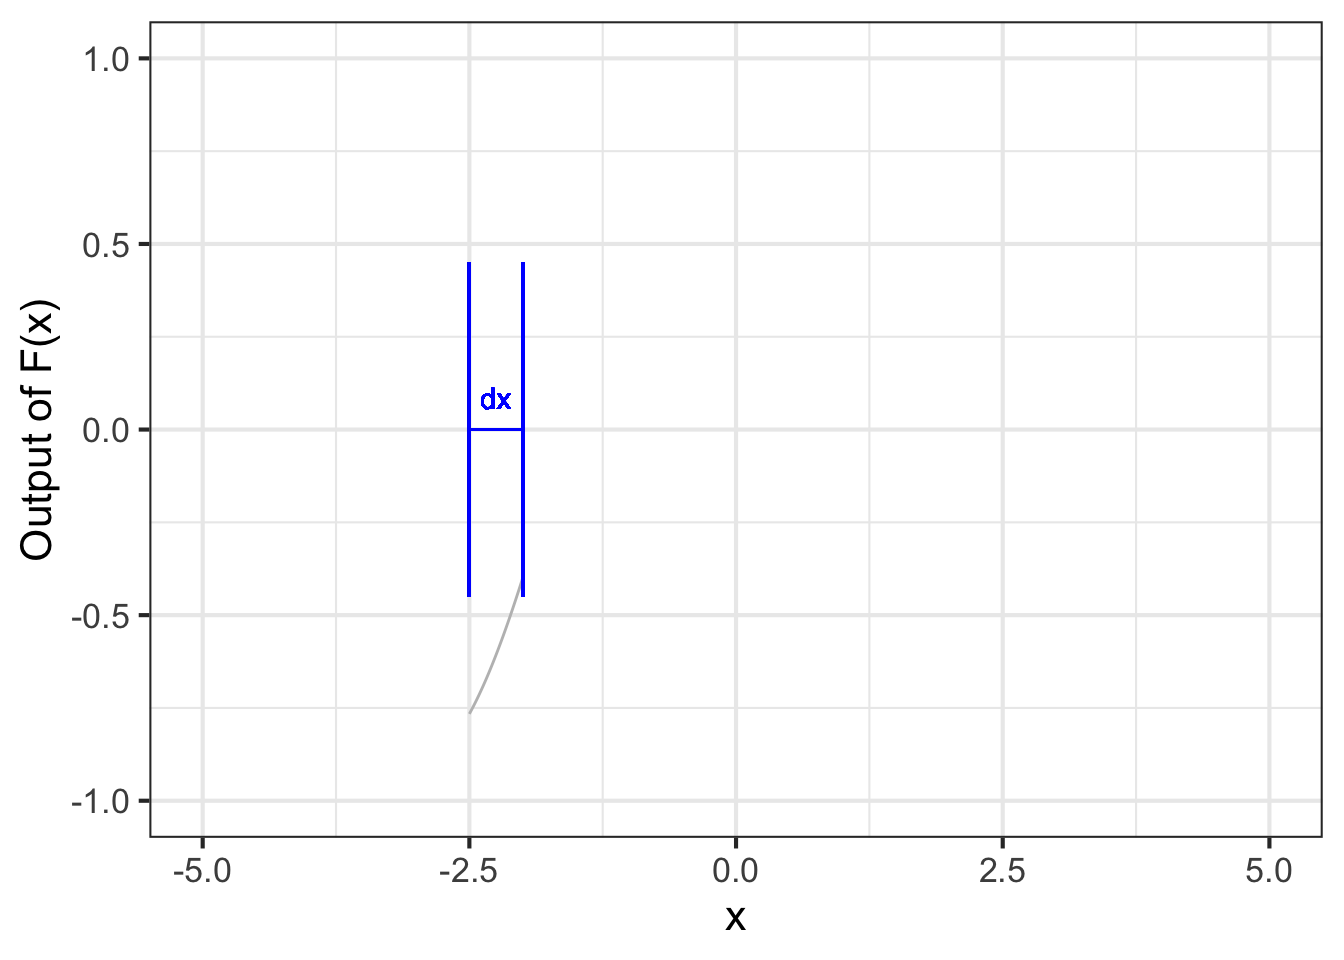
\includegraphics[width=0.9\textwidth,height=\textheight]{Accumulation/28-visualizing_files/figure-pdf/fig-F-blank-axes-1.pdf}

}

\caption{\label{fig-F-blank-axes}The graphics frame in which we want to
draw the graph of \(F(x)\). A small region of the domain is labeled
\(dx\). Within that domain, \(F(x)\), whatever it is, will be a sloping
segment. The gray segment shows what this might look like.}

\end{figure}

It's premature to have drawn a segment of \(F(x)\) because we haven't
yet undertaken to compute \(F(x) = \int f(x)\, dx\). At this point in
the process, all we know is \(f(x)\), not \(F(x)\). Still, since we know
\(f(x)\), we do know the slope of the little segment of \(F(x)\). We
just don't know where that segment should be located vertically in each
of the \(dx\) regions that make up the whole domain.

We can't draw \(f(x)\) in the ordinary way as a curve wending its way
across the domain of the graph. Why not? Because the vertical axis of
the graphics frame is in terms of \(F(x)\) and has a different dimension
than the output of \(f(x)\).

But we can draw \(f(x)\) in terms of the slope of a segment of
horizontal extent \(dx\), so long as we accept that the vertical
position of that segment means nothing: \(f(x)\) gives information only
about the \textbf{slope} of the segment. The best we can do at this
point is to graph \(f(x)\) in terms of sloping segments, as in
\textbf{?@fig-f-blank-axes2}.

\begin{figure}

\sidecaption{\label{fig-F-blank-axes2}Graphing \(f(x)\) as a series of
sloped segments. The slope is the value of \(f(x)\). But the vertical
position of the segment is not information provided by \(f(x)\), so
we've drawn all of them at the same vertical level.}

{\centering 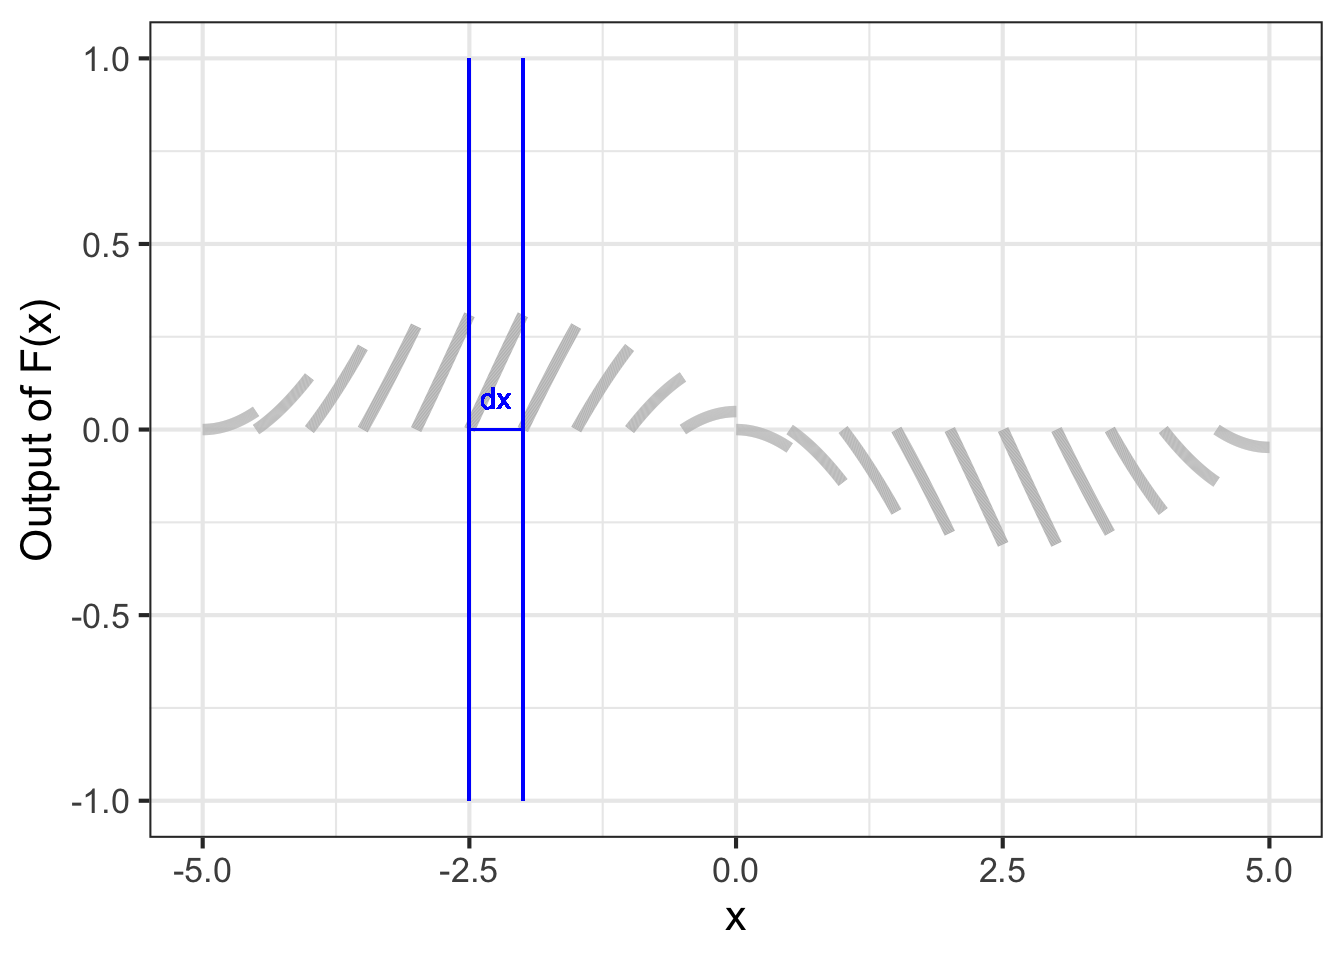
\includegraphics[width=0.9\textwidth,height=\textheight]{Accumulation/28-visualizing_files/figure-pdf/fig-F-blank-axes2-1.pdf}

}

\end{figure}

Each of the segments in \textbf{?@fig-f-blank-axes2} has the same
horizontal extent, namely \(dx\). When we draw a sloping segment over
the tiny bit \(dx\) of the domain, the vertical extent of the segment
will be the product of the width \(dx\) and the slope \(f(x)\). That is,
the vertical extent will be the product \(f(x) dx\).

Whenever we know a function \(f(x)\) and have chosen a size for \(dx\)
we can draw a graph of \(f(x)\) in the form shown in
\textbf{?@fig-f-blank-axes2}. We're drawing it in this unusual way
because we want the graphics frame to be all ready for drawing the graph
of \(F(x)\) in the normal fashion after we have figured out what
\(F(x)\) results from accumulating/summing-up all the little \(f(x) dx\)
segments. When we write \(\large\int\) in the notation
\[\large \int f(x)\, dx\] we mean, ``sum up all the \(f(x) dx\)
segments.''

Let's now consider how to ``sum up all the segments.'' We'll start in
\textbf{?@fig-f-232} with an example where we already know \(F(x)\).
That way, we can see of our sum of the \(f(x) dx\) segments really does
reconstruct \(F(x)\).

\begin{figure}

\sidecaption{\label{fig-F-232}Top: A function \(F(x)\) for demonstration
purposes. Bottom: Slicing \(F(x)\) into piecewise domains of width
\(dx=2\) and anchoring the left-most point of each slice vertically at
0.}

{\centering 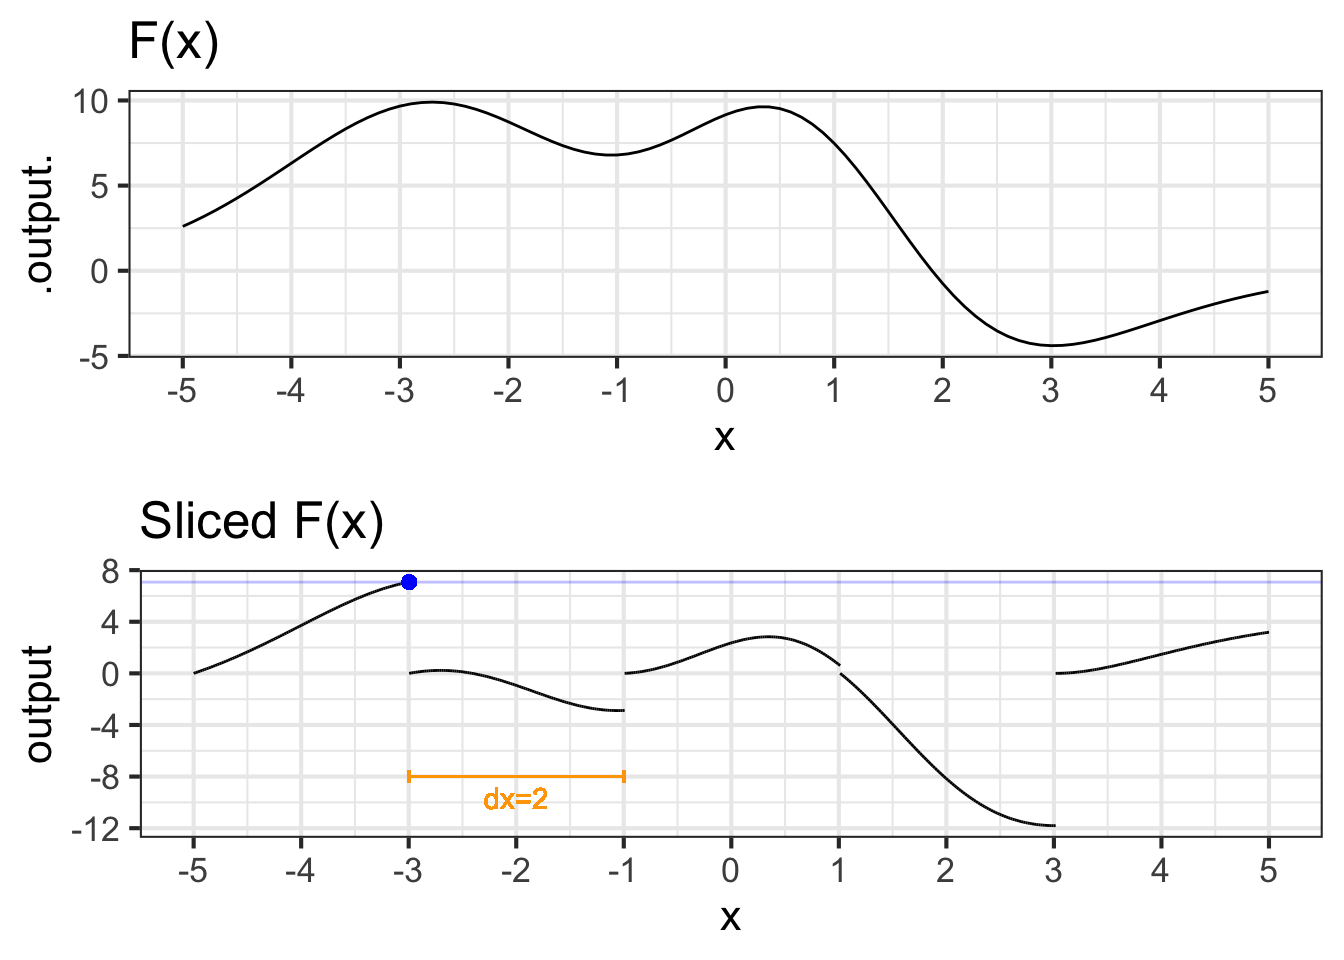
\includegraphics[width=0.9\textwidth,height=\textheight]{Accumulation/28-visualizing_files/figure-pdf/fig-F-232-1.pdf}

}

\end{figure}

Now imagine that we sliced up \(F(x)\) over small sub-domains of \(x\),
as in \textbf{?@fig-f-232} (bottom). That is, we approximated \(F()\)
piecewise locally. But we've broken the continuity of \(F(x)\) by moving
each slice up or down so that the left-most point has value 0.

Can you reconstruct \(F(x)\) from the local segments?

Start by reading off the function value from the last point in the
left-most segment. That's been marked in \textbf{?@fig-f-232} with a
blue dot. The function value at that dot is 7.072.

Now take the second segment. The idea is to move that segment upward
until it joins the first segment at the blue dot. You can do that by
adding 7.072 to the second segment. The result is shown in
\textbf{?@fig-f-seg-2}(top).

\begin{figure}

\sidecaption{\label{fig-F-seg-2}Reconstructing the original function
\(F(x)\) by moving each segment upward to meet its left neighbor. Top:
The first two segments are connected. Bottom: The third segment is
connected to the first two.}

{\centering 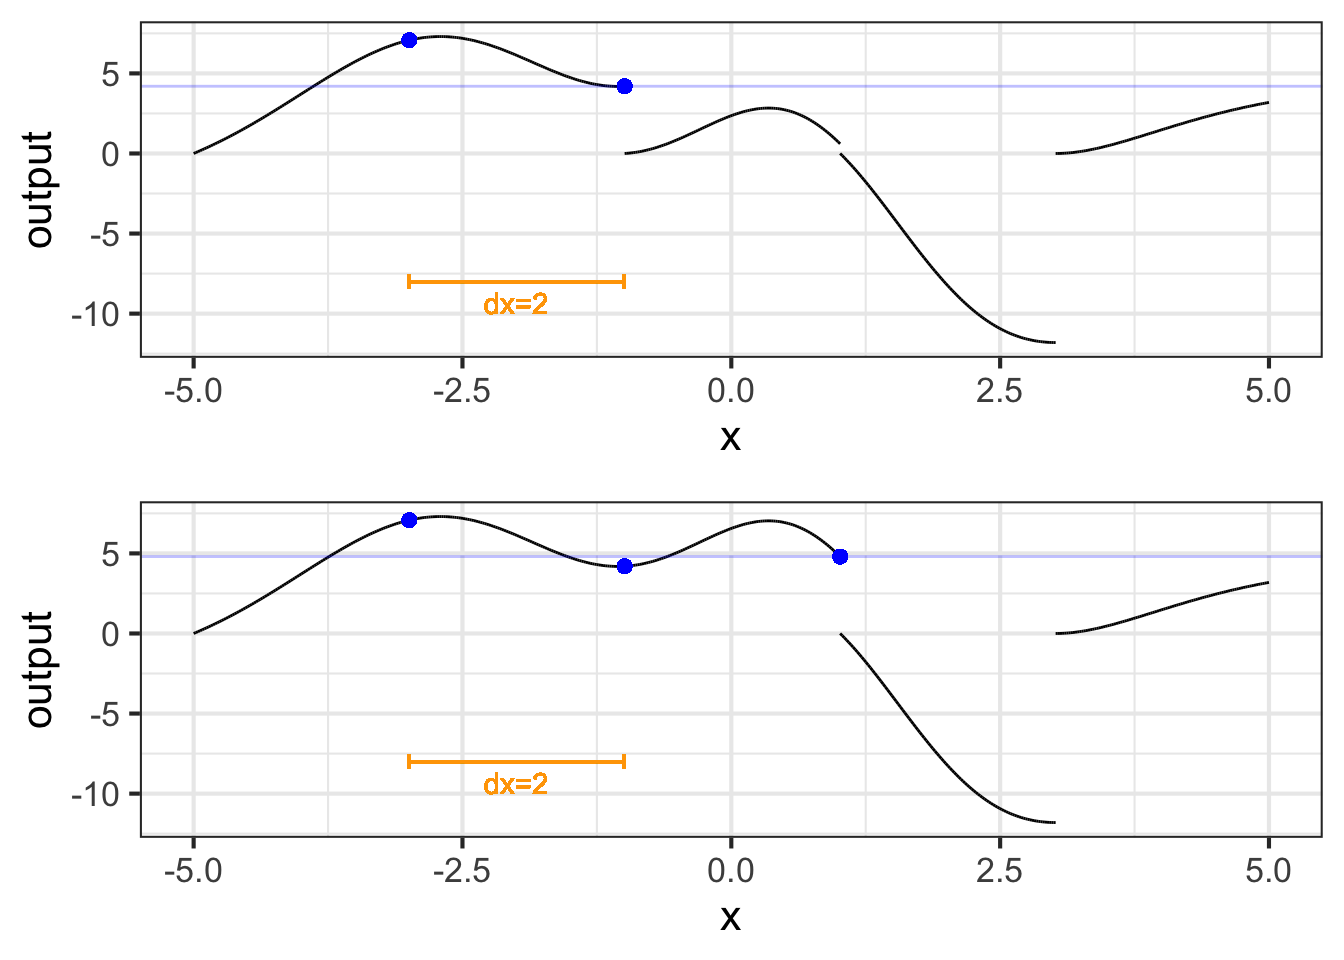
\includegraphics[width=0.9\textwidth,height=\textheight]{Accumulation/28-visualizing_files/figure-pdf/fig-F-seg-2-1.pdf}

}

\end{figure}

Now read off the new value at the end of the second segment, it's 4.198.
Add this amount to the third segment as in
\textbf{?@fig-f-seg-2}(bottom).

Continue this process until you have reconstructed \(F(x)\) from the
local segments.

You may object: ``Of course you can reconstruct \(F(x)\) from the local
segments, but this isn't the same as reconstructing \(F(x)\) from its
derivative \(\partial_x F(x)\).'' My answer: ``That depends on how many
segments you use.''

When we make the segment width \(h\) smaller and smaller, the individual
segments become more and more like straight lines.
\textbf{?@fig-f-slice-many} shows the segments for smaller and smaller
\(h\).

\begin{figure}

\sidecaption{\label{fig-F-slice-many}Using small segments gives each
segment a simple shape. In Figure @ref(fig:F-seg-2) the segments had
width \(dx=2.0\) and were discernable curvy. Top of this figure: At
width \(dx=0.25\) a few of the segments look curved. Middle: This graph
zooms in on the subdomain \(-1 \leq x \leq 1\) in the top panel, where
there is a notably curved segment in the top graph. Setting \(dx=0.1\)
breaks up such curved segment into components better approximated by a
straight line. Bottom: Using \(dx=0.01\) further improves the
approximation of each segment to a straight line.}

{\centering 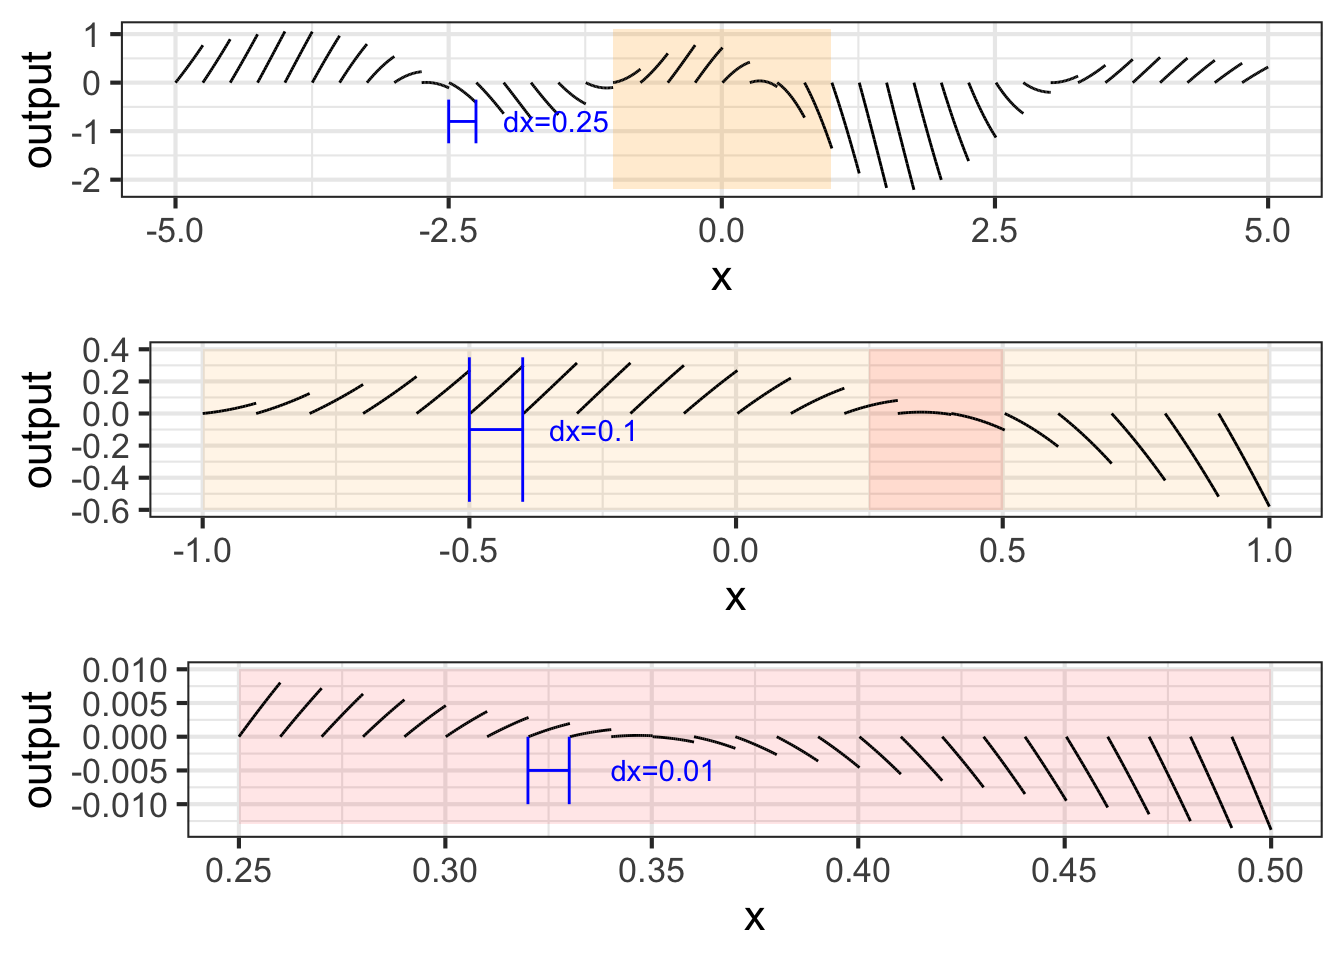
\includegraphics[width=0.9\textwidth,height=\textheight]{Accumulation/28-visualizing_files/figure-pdf/fig-F-slice-many-1.pdf}

}

\end{figure}

Notice that many of the segments are straight lines. That's
understandable, since any function looks like a straight line over a
small enough domain.

Each of those straight-line segments is drawn over a domain
\(x_i < x < x_i+dx\) that has width \(dx\). For \(dx\) small enough, the
segment is well approximated by a straight line with slope
\(\partial_x F(x_i)\). Multiplying slope by width \(dx\) gives the
segment height: \(\left[{\large\strut}\partial_x F(x_i)\right]\ dx\). Of
course, remember that \(\partial_x F(x) = f(x)\) helps us see that each
of the little segments is \(f(x_i)\ dx\).

Lets review. The standard notation for anti-differentiation can be
interpreted in terms of putting together segments, or, in the words of
Prof.~Thompson in \emph{Calculus Made Easy}, ``totaling up all the
little bits.'' (See Section~\ref{sec-preliminary-terrors}.)

\begin{enumerate}
\def\labelenumi{\arabic{enumi}.}
\item
  We start with the function that we already know: \(\large f(x)\).
  Remember that \(f(x)\), at each value of \(x\) will be the
  \emph{slope} of \(F(x)\). Why? Because \(F(x)\) is the anti-derivative
  of \(f(x)\), so \(f(x)\) is the derivative of \(F(x)\).
\item
  Now divide the domain \(x\) into many little bits. Each of these
  sub-domains is \(\large dx\), a little chunk of \(x\).
\item
  On each of the little chunks, draw in \(f(x)\). Since \(f(x)\) is the
  \emph{slope} of \(F(x)\), we will draw \(f(x)\) for any given chunk as
  a short line segment of that slope over the chunk, as in
  \textbf{?@fig-f-blank-axes2}. We'll write these little bits, each of
  which is very nearly a straight-line, as
  \(\large\color{blue}{f(x) dx}\).
\item
  Assemble together all the \(f(x)dx\) segments from (3) to get
  \(F(x)\). This instruction to assemble is denoted
  \[\Large \color{blue}\int\]
\end{enumerate}

Altogether, we have:

\[\large \underbrace{\underbrace{\Large\color{magenta}{\int}}_{\color{magenta}{\text{assemble}}} \underbrace{\Large \overbrace{f(x)}^{\small\text{slope of F(x)}}\ \  \overbrace{\strut dx}^{\small \text{bits of}\ x}}_{\color{blue}{\text{the slope segments}}}}_{\text{giving}\ {\Large F(x)+C}\ \text{altogether.}}\]

\begin{example}

Returning to the example with which we started the chapter, here are the
little segments of the slope function shown in
\textbf{?@fig-f-blank-axes2} assembled together to produce the
anti-derivative function.

\begin{figure}

{\centering 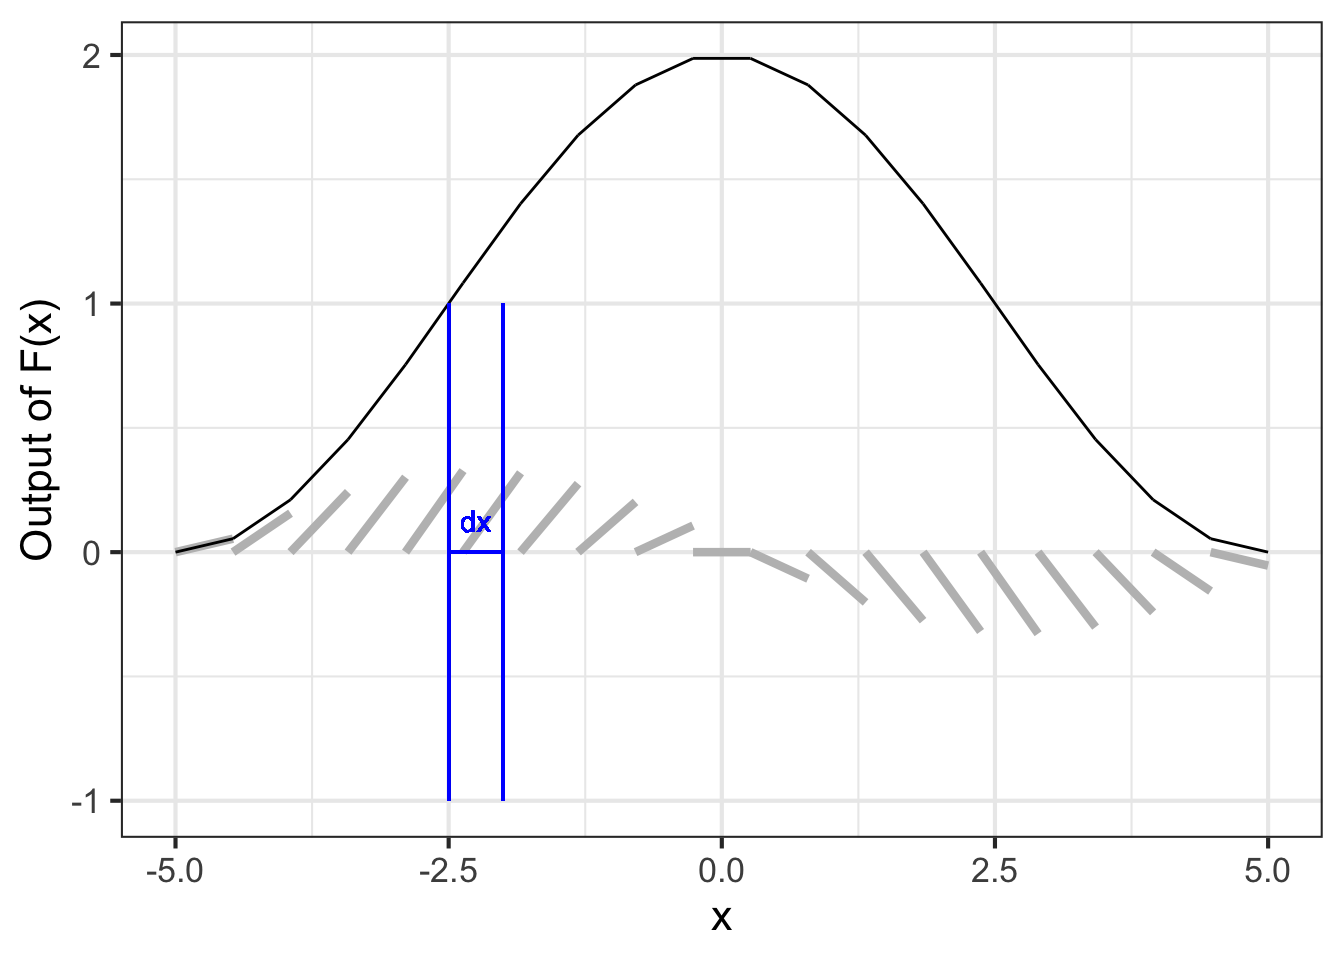
\includegraphics[width=0.9\textwidth,height=\textheight]{Accumulation/28-visualizing_files/figure-pdf/fig-show-bits2-1.pdf}

}

\caption{\label{fig-show-bits2}\(\color{blue}{\int} f(x)dx\) means to
assemble the straight-line pieces \(f(x) dx\) in the manner described in
the previous section.}

\end{figure}

\end{example}

\hypertarget{exercises-1}{%
\section{Exercises}\label{exercises-1}}

\hypertarget{sec-net-change}{%
\chapter{Integration}\label{sec-net-change}}

Anti-derivatives are useful when you know how a quantity is changing but
don't yet know the quantity itself.

It's important, of course, to keep track of which is the ``quantity
itself'' and which is the ``rate of increase in that quantity.'' This
always depends on context and your point of view. It's convenient, then,
to set some fixed examples to make it easy to keep track of which
quantity is which.

\begin{longtable}[]{@{}
  >{\raggedright\arraybackslash}p{(\columnwidth - 4\tabcolsep) * \real{0.1600}}
  >{\raggedright\arraybackslash}p{(\columnwidth - 4\tabcolsep) * \real{0.4400}}
  >{\raggedright\arraybackslash}p{(\columnwidth - 4\tabcolsep) * \real{0.4000}}@{}}
\toprule
\begin{minipage}[b]{\linewidth}\raggedright
Context
\end{minipage} & \begin{minipage}[b]{\linewidth}\raggedright
Quantity
\end{minipage} & \begin{minipage}[b]{\linewidth}\raggedright
Rate of increase in quantity
\end{minipage} \\
\midrule
\endhead
Money & Cash on hand \({\mathbf S}(t)\) & Cash flow \(s(t)\) \\
Fuel & Amount in fuel tank \({\mathbf F}(t)\) & Fuel consumption rate,
e.g.~kg/hour \(f(t)\) \\
Motion & Momentum \({\mathbf M}(t)\) & Force \(m(t)\) \\
notation & \({\mathbf H}(t)\) & \(\partial_t {\mathbf H}(t)\) \\
notation & \(G(t) = \int g(t) dt\) & \(g(t)\) \\
\bottomrule
\end{longtable}

We'll also adopt a convention to make it simpler to recognize which
quantity is the ``quantity itself'' and which is the ``rate of increase
in that quantity.'' We will use CAPITAL LETTERS to name functions that
are the quantity itself, and \emph{lower-case} letters for the rate of
increase in that quantity. For example, if talking about motion, an
important quantity is \textbf{\emph{momentum}} and how it changes over
time. The momentum itself will be \({\mathbf M}(t)\) while the rate of
increase of momentum will be \(m(t)\).\sidenote{\footnotesize Momentum is velocity
  times mass. Newton's Second Law of Motion stipulates that force equals
  the rate of change of momentum.} The amount of money a business has on
hand at time \(t\) is \({\mathbf S}(t)\) measured, say, in dollars. The
rate of increase of that money is \(s(t)\), in, say, dollars per day.

Notice that we're using the phrase ``rate of increase'' rather than
``rate of change.'' That's because we want to keep straight the meaning
of the sign of the \emph{lower-case} function. If \(m(t)\) is positive,
the momentum is increasing. If \(m(t)\) is negative then it's a
``negative rate of increase,'' which is, of course, just a ``decrease.''

For a business, money coming in means that \(s(t)\) is positive.
Expenditures of money correspond to \(s(t)\) being negative. In the fuel
example. \({\mathbf F}(t)\) is the amount of fuel in the tank. \(f(t)\)
is the rate of \emph{increase} in the amount of fuel in the tank. Of
course, engines burn fuel, removing it from the tank. So we would write
the rate at which fuel is burned as \(-f(t)\): removing fuel is a
negative increase in the amount of fuel, an expenditure of fuel.

The objective of this chapter is to introduce you to the sorts of
calculations, and their notations, that let you figure out how much the
CAPITAL LETTER quantity has changed over an interval of \(t\) based on
what you already know about the value over time of the \emph{lower-case}
function.

The first step in any such calculation is to find or construct the
\emph{lower-case} function \(f(t)\) or \(c(t)\) or \(m(t)\) or whatever
it might be. This is a modeling phase. In this chapter, we'll ignore
detailed modeling of the situation and just present you with the
\emph{lower-case} function.

The second step in any such calculation is to compute the
anti-derivative of the \emph{lower-case} function, giving as a result
the CAPITAL LETTER function. You've already seen the notation for this,
e.g.
\[{\Large  F(t) = \int f(t) dt}\ \ \ \ \ \text{or}\ \ \ \ \ {\Large G(t) = \int g(t) dt}\ \ \ \ \text{and so on.}\]
In this chapter, we will not spend any time on this step; we will assume
that you already have at hand the means to compute the anti-derivative.
(Indeed, you already have \texttt{antiD()} available which will do the
job for you.) Later chapters will look at the issues around and
techniques for doing the computations by other means.

The remaining steps in such calculations are to work with the CAPITAL
LETTER function to compute such things as the amount of that quantity,
or the change in that quantity as it is accumulated over an interval of
\(t\).

\begin{why}
Sometimes you're writing the capital letter functions in
\textbf{bold-face}, e.g.~\({\mathbf F}(t)\) and other times you aren't,
e.g.~\(F(t)\). What's going on?

This is a convention we're adopting for this chapter, which is when we
need it the most to introduce the concepts.

\textbf{Bold-face} is being used in this chapter to represent the
real-world quantity of interest. So \({\mathbf F}(t)\) is the actual
amount of fuel in the tank, \({\mathbf M}(t)\) is the actual momentum of
the car, and \({\mathbf S}(t)\) is the actual amount of money on hand.
The regular-face functions, \(F(t)\) and \(M(t)\) and \(S(t)\) are the
functions that we get by applying anti-differentiation to \(f(t)\) or
\(m(t)\) or \(s(t)\).

Our broad interest is to construct the \textbf{bold-face} function
knowing just the derivative of that function, which we're writing in
\emph{lower-case}. So, \(f(t) \equiv \partial_t {\mathbf F}(t)\).
Similarly, \(m(t) \equiv \partial_t {\mathbf M}(t)\) and
\(s(t) \equiv \partial_t {\mathbf S}(t)\).

If we knew \({\mathbf F}(t)\) or \({\mathbf M}(t)\) or
\({\mathbf S}(t)\), that would be the end of the matter, since our
interest is in the quantity \({\mathbf F}\) or \({\mathbf V}\) or
\({\mathbf M}\). But we are working with a situation where we know
\(f(t)\) but not \({\mathbf F}(t)\), or we know \(m(t)\) but not
\({\mathbf M}(t)\), and so on.

How could such a situation arise in the real world? Suppose the car's
fuel gauge is broken, depriving us of direct knowledge of \(\mathbf F\),
but that we have a dashboard readout of the rate of fuel consumption.
Then we would know \(f(t)\) but not \({\mathbf F}(t)\). Or suppose you
are in charge of day-to-day running of a business, collecting the income
each day and paying the daily expenses. Thus, each day you know
\(s(t)\)---the cash flow. But it's your boss who has access to the bank
account; you merely deposit money as you get it and write checks or
Venmo suppliers (or however it is that your business operates day to
day). So your boss knows \({\mathbf S}(t)\) but you know only \(s(t)\).

Since you know about anti-differentiation, you can try to reconstruct
the fuel level \({\mathbf F}(t)\) from the known \(f(t)\), or to figure
out the bank balance \({\mathbf S}(t)\) from your records of \(s(t)\).

But anti-differentiation, while part of the solution, is only just a
part. You can apply anti-differentiation to \(f(t)\), but what you get
back will be \(F(t)\), not \({\mathbf F}(t)\).

What's the difference between the two? It involves a constant value
\(C\) which, alas, you can never figure out from \(f(t)\). All that you
can claim, given the \(F(t)\) generated by anti-differentiation, is that
\[{\mathbf F}(t) = F(t) + C .\]

\end{why}

\hypertarget{net-change}{%
\section{Net change}\label{net-change}}

Perhaps it goes without saying, but once you have the CAPITAL LETTER
function, e.g.~\(F(t)\), you can evaluate that function at any input
that falls into the domain of \(F(t)\). If you have a graph of \(F(t)\)
versus \(t\), just position your finger on the horizontal axis at input
\(t_1\), then trace up to the function graph, then horizontally to the
vertical axis where you can read off the value \(F(t_1)\). If you have
\(F()\) in the form of a computer function, just \textbf{\emph{apply}}
\(F()\) to the input \(t_1\).

In this regard, \(F(t)\) is like any other function.

However, in using and interpreting the \(F(t)\) that we constructed by
anti-differentiating \(f(t)\), we have to keep in mind the limitations
of the anti-differentiation process. In particular, any function
\(f(t)\) does not have a unique anti-derivative function. If we have one
anti-derivative, we can always construct another by adding some
constant: \(F(t) + C\) is also an anti-derivative of \(f(t)\).

But we have a special purpose in mind when calculating \(F(t_1)\). We
want to figure out from \(F(t)\) how much of the quantity \(f(t)\) has
accumulated up to time \(t_1\). For example, if \(f(t)\) is the rate of
increase in fuel (that is, the negative of fuel consumption), we want
\(F(t_1)\) to be the amount of fuel in our tank at time \(t_1\).
\textbf{That cannot happen.} All we can say is that \(F(t_1)\) is the
amount of fuel in the tank at \(t_1\) give or take some unknown constant
C.

Instead, the correct use of \(F(t)\) is to say how much the quantity has
changed over some interval of time, \(t_0 \leq t \leq t_1\). This
``change in the quantity'' is called the \textbf{\emph{net change}} in
\(F()\). To calculate the net change in \(F()\) from \(t_0\) to \(t_1\)
we apply \(F()\) to both \(t_0\) and \(t_1\), then subtract:

\[\text{Net change in}\ F(t) \ \text{from}\ t_0 \ \text{to}\ t_1 :\\= F(t_1) - F(t_0)\]

\begin{example}
Suppose you have already constructed the rate-of-change function for
momentum \(m()\) and implemented it as an R function \texttt{m()}. For
instance, \(m(t)\) might be the amount of \textbf{force} at any instant
\(t\) of a car, and \({\mathbf M}(t)\) is the \textbf{accumulated
force}, better known as momentum. We'll assume that the input to
\texttt{m()} is in seconds, and the output is in
kg-meters-per-second-squared, which has the correct dimension for force.

You want to find the amount of force accumulated between time \(t=2\)
and \(t=5\) seconds.

\begin{Shaded}
\begin{Highlighting}[]
\CommentTok{\# You\textquotesingle{}ve previous constructed m(t)}
\NormalTok{M }\OtherTok{\textless{}{-}} \FunctionTok{antiD}\NormalTok{(}\FunctionTok{m}\NormalTok{(t) }\SpecialCharTok{\textasciitilde{}}\NormalTok{ t)}
\FunctionTok{M}\NormalTok{(}\DecValTok{5}\NormalTok{) }\SpecialCharTok{{-}} \FunctionTok{M}\NormalTok{(}\DecValTok{2}\NormalTok{)}
\DocumentationTok{\#\# [1] {-}1.392131}
\end{Highlighting}
\end{Shaded}

To make use of this quantity, you'll need to know it's dimension and
units. For this example, where the dimension {[}\(m(t)\){]} is M L
T\(^{-2}\), and {[}\(t\){]} = T, the dimension {[}\({\mathbf M}(t)\){]}
will be M L T\(^{-1}\). In other words, if the output of \(m(t)\) is
kg-meters-per-second-squared, then the output of \(V(t)\) must be kg-
meters-per-second.

\end{example}

\hypertarget{the-definite-integral}{%
\section{The ``definite'' integral}\label{the-definite-integral}}

We have described the process of calculating a net change from the
\emph{lower-case} function \(f(t)\) in terms of two steps:

\begin{enumerate}
\def\labelenumi{\arabic{enumi}.}
\tightlist
\item
  Construct \(F(t) = \int f(t) dt\).
\item
  Evaluate \(F(t)\) at two inputs, e.g.~\(F(t_2) - F(t_1)\), giving a
  net change, which we'll write as
  \({\cal F}(t_1, t_2) = F(t_2) - F(t_1)\).
\end{enumerate}

As a matter of notation, the process of going from \(f(t)\) to the net
change is written as one statement.
\[{\cal F}(t_1, t_2) = F(t_2) - F(t_1) = \int_{t_1}^{t_2} f(t) dt\]

The punctuation \[\int_{t_1}^{t_2} \_\_\_\_ dt\] captures in one
construction both the anti-differentiation step (\(\int\_\_dt\)) and the
evaluation of the anti-derivative at the two bound \(t_2\) and \(t_1\).

Several names are used to describe the overall process. It is important
to become familiar with these.

\begin{itemize}
\tightlist
\item
  \(\int_a^b f(t) dt\) is called a \textbf{\emph{definite integral}} of
  \(f(t)\).
\item
  \(a\) and \(b\) are called, respectively, the \textbf{\emph{lower
  bound of integration}} and the \textbf{\emph{upper bound of
  integration}}, although given the way we draw graphs it might be
  better to call them the ``left'' and ``right'' bounds, rather than
  lower and upper.
\item
  The pair \(a, b\) is called the \textbf{\emph{bounds of integration}}.
\end{itemize}

As always, it pays to know what \emph{kind of thing} is
\({\cal F}(t_1, t_2)\). Assuming that \(t_1\) and \(t_2\) are fixed
quantities, say \(t_1 = 2\) seconds and \(t_2 = 5\) seconds, then
\({\cal F}(t_1, t_2)\) is itself a quantity. The dimension of that
quantity is {[}\(F(t)\){]} which in turn is
{[}\(f(t)\){]}\(\cdot\){[}\(t\){]}. So if \(f(t)\) is fuel consumption
in liters per second, then \(F(t)\) will have units of liters, and
\({\cal F}(t_1, t_2)\) will also have units of liters.

Remember also an important distinction:

\begin{itemize}
\tightlist
\item
  \(F(t) = \int f(t) dt\) is a \textbf{\emph{function}} whose output is
  a quantity.
\item
  \(F(t_2) - F(t_1) = \int_{t_1}^{t_2} f(t) dt\) is a
  \textbf{\emph{quantity}}, not a function.
\end{itemize}

Of course, \(f(t)\) is a \textbf{\emph{function}} whose output is a
quantity. In general, the two functions \(F(t)\) and \(f(t)\) produce
outputs that are \emph{different kinds} of quantities. For instance, the
output of \(F(t)\) is liters of fuel while the output of \(f(t)\) is
liters per second: fuel consumption. Similarly, the output of \(S(t)\)
is dollars, while the output of \(s(t)\) is dollars per day.

The use of the term \textbf{\emph{definite integral}} suggests that
there might be something called an \textbf{\emph{indefinite integral}},
and indeed there is. ``Indefinite integral'' is just a synonym for
``anti-derivative.'' In this book we favor the use of
\textbf{\emph{anti-derivative}} because it's too easy to leave off the
``indefinite'' and confuse an indefinite integral with a definite
integral. Also, ``anti-derivative'' makes it completely clear what is
the relationship to ``derivative.''

Since 1700, it's common for calculus courses to be organized into two
divisions:

\begin{enumerate}
\def\labelenumi{\roman{enumi}.}
\tightlist
\item
  Differential calculus, which is the study of derivatives and their
  uses.
\item
  Integral calculus, which is the study of anti-derivatives and their
  uses.
\end{enumerate}

Mathematical notation having been developed for experts rather than for
students, very small typographical changes are often used to signal very
large changes in meaning. When it comes to anti-differentiation, there
are two poles of fixed meaning and then small changes which modify the
meaning. The poles are:

\begin{enumerate}
\def\labelenumi{\roman{enumi}.}
\tightlist
\item
  Anti-derivative: \(\int f(t) dt\), which is a function whose output is
  a quantity.
\item
  Definite integral \(\int_a^b f(t) dt\), which is a quantity, plain and
  simple.
\end{enumerate}

But you will also see some intermediate forms:

\begin{enumerate}
\def\labelenumi{\alph{enumi}.}
\item
  \(\int_a^t f(t) dt\), which is a \textbf{function} with input \(t\).
\item
  \(\int_a^x f(t) dt\), which is the same function as in (a) but with
  the input name \(x\) being used.
\item
  \(\int_t^b f(t) dt\), which is a \textbf{function} with input \(t\).
\item
  Less commonly, \(\int_x^t f(t) dt\) which is a \textbf{function} with
  two inputs, \(x\) and \(t\). The same is true of \(\int_x^y f(t) dt\)
  and similar variations.
\end{enumerate}

\hypertarget{initial-value-of-the-quantity}{%
\section{Initial value of the
quantity}\label{initial-value-of-the-quantity}}

Recall that we're interested in a real quantity \({\mathbf F}(t)\), but
we only know \(f(t)\) and from that can calculate an anti-derivative
\(F(t)\). The relationship between them is \[{\mathbf F}(t) = F(t) + C\]
where \(C\) is some fixed quantity that we cannot determine directly
from \(f(t)\).

Still, even if we cannot determine \(C\), there's one way we can use
\(F(t)\) to make definite statements about \({\mathbf F}(t)\). Consider
the net change from \(t_1\) to \(t_2\) in the real quantity
\({\mathbf F}\). This is
\[{\mathbf F}(t_2) - {\mathbf F}(t_1) =  \left[F(t_2) + C\right] - \left[F(t_1) + C\right] = F(t_2) - F(t_1)\]
In other words, just knowing \(F(t)\), we can make completely accurate
statements about net changes in the value of \({\mathbf F}(t)\).

Let's develop our understanding of this unknown constant \(C\), which is
called the \textbf{\emph{constant of integration}}. To do so, watch the
movie in Figure~\ref{fig-accum-movie-1} showing the process of
constructing the anti-derivative \[F(t) = \int_2^t f(t) dt\ .\]

\begin{figure}

\sidecaption{\label{fig-accum-movie-1}Constructing the anti-derivative
\(F(t)\) by reading the slope from \(f(t)\) and using that slope to
extend the picture of \(F()\)}

{\centering 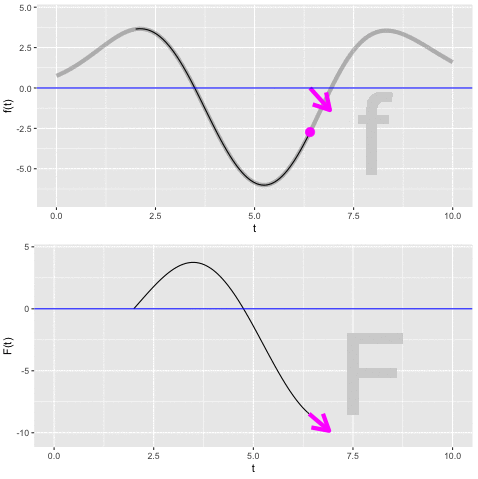
\includegraphics[width=0.9\textwidth,height=\textheight]{Accumulation/www/arrow-plot-still.png}

}

\end{figure}

\begin{enumerate}
\def\labelenumi{\arabic{enumi}.}
\tightlist
\item
  Focus first on the top graph. The function we are integrating,
  \(f(t)\), is known before we carry out the integration, so it is shown
  in the top graph.
\end{enumerate}

\(f(t)\) is the rate of increase in \(F(t)\) (or \({\mathbf F}(t)\) for
that matter). From the graph, you can read using the vertical axis the
value of \(f(t)\) for any input \(t\). But since \(f(t)\) is a rate of
increase, we can also depict \(f(t)\) as a slope. That slope is being
drawn as a \(\color{magenta}{\text{magenta}}\) arrow. Notice that when
\(f(t)\) is positive, the arrow slopes upward and when \(f(t)\) is
negative, the arrow slopes downward. The steepness of the arrow is the
value of \(f(t)\), so for inputs where the value of \(f(t)\) is far from
zero the arrow is steeper than for values of \(f(t)\) that are near
zero.

\begin{enumerate}
\def\labelenumi{\arabic{enumi}.}
\setcounter{enumi}{1}
\item
  Now look at both graphs, but concentrate just on the arrows in the two
  graphs. They are always the same: carbon copies of one another.
\item
  Finally the bottom graph. We're starting the integral at \(t_1=2\).
  Since nothing has yet been accumulated, the value \(F(t_1 = 2) = 0\).
  From (1) and (2), you know the arrow shows the slope of \(F(t)\). So
  as \(F(t>2)\) is being constructed the arrow guides the way. When the
  slope arrow is positive, \(F(t)\) is growing. When the slope arrow is
  negative, \(F(t)\) is going down.
\end{enumerate}

In tallying up the accumulation of \(f(t)\), we started at time \(t=2\)
and with \(F(t=2) = 0\). This makes sense, since nothing can be
accumulated over the mere instant of time from \(t=2\) to \(t=2\). On
the other hand, it was our choice to start at \(t=2\). We might have
started at another value of \(t\) such as \(t=0\) or \(t=-5\) or
\(t=-\infty\). If so, then the accumulation of \(f(t)\) up to \(t=2\)
would likely have been something other than zero.

But what if we knew an actual value for \({\mathbf F}(2)\). This is
often the case. For instance, before taking a trip you might have filled
up the fuel tank. The accumulation of fuel consumption only tells you
how much fuel has been used since the start of the trip. But if you know
the starting amount of fuel, by adding that to the accumulation you'll
know instant by instant how much fuel is in the tank. In other words,
\[{\mathbf F}(t) = {\mathbf F}(2) + \int_2^t f(t) dt\ .\] This is why,
when we write an anti-derivative, we should always include mention of
some constant \(C\)---the so-called \textbf{\emph{constant of
integration}}---to remind us that there is a difference between the
\(F(t)\) we get from anti-differentiation and the \({\mathbf F}(t)\) of
the function we're trying to reconstruct. That is,
\[{\mathbf F}(t) = F(t) + C = \int f(t) dt + C\ .\] We only need to know
\({\mathbf F}(t)\) at one point in time, say \(t=0\), to be able to
figure out the value of \(C\): \[C = {\mathbf F}(0) - F(0)\ .\]

Another way to state the relationship between the anti-derivative and
\({\mathbf F}(t)\) is by using the anti-derivative to accumulate
\(f(t)\) from some starting point \(t_0\) to time \(t\). That is:
\[{\mathbf F}(t) \ =\  {\mathbf F}(t_0) + \int_{t_0}^t f(t)\, dt\  = \ 
{\mathbf F}(t_0) + \left({\large\strut}F(t) - F(t_0)\right)\]

A famous legend has Galileo at the top of the Tower of Pisa around 1590.
The legend illustrates Galileo's finding that a light object (e.g.~a
marble) and a heavy object (e.g.~a ball) will fall at the same speed.
Galileo published his mathematical findings in 1638 in \emph{Discorsi e
Dimostrazioni Matematiche, intorno a due nuove scienze}. (English:
Discourses and Mathematical Demonstrations Relating to Two New Sciences)

In 1687, Newton published his world-changing\emph{Philosophiae Naturalis
Principia Mathematica}. (English: Mathematical Principles of Natural
Philosophy)

Let's imagine the ghost of Galileo returned to Pisa in 1690 after
reading Newton's \emph{Principia Mathematica}. In this new legend,
Galileo holds a ball still in his hand, releases it, and figures out the
position of the ball as a function of time.

Although Newton famously demonstrated that gravitational attraction is a
function of the distance between to objects, he also knew that at a
fixed distance---the surface of the Earth---gravitational acceleration
was constant. So Galileo was vindicated by Newton. But, although
gravitational acceleration is constant from top to bottom of the Tower
of Pisa, Galileo's ball was part of a more complex system: a hand
holding the ball still until release. Acceleration of the ball versus
time is therefore approximately a Heaviside function:

\[\text{accel}(t) \equiv \left\{\begin{array}{rl}0 & \text{for}\ t \leq 3\\
{-9.8}  & \text{otherwise}\end{array}\right.\]

\begin{Shaded}
\begin{Highlighting}[]
\NormalTok{accel }\OtherTok{\textless{}{-}} \FunctionTok{makeFun}\NormalTok{(}\FunctionTok{ifelse}\NormalTok{(t }\SpecialCharTok{\textless{}=} \DecValTok{3}\NormalTok{, }\DecValTok{0}\NormalTok{, }\SpecialCharTok{{-}}\FloatTok{9.8}\NormalTok{) }\SpecialCharTok{\textasciitilde{}}\NormalTok{ t)}
\end{Highlighting}
\end{Shaded}

Acceleration is the derivative of velocity. We can construct a function
\(V(t)\) as the anti-derivative of acceleration, but the real-world
velocity function will be
\[{\mathbf V}(t) = {\mathbf V}(0) + \int_0^t \text{accel}(t) dt\]

\begin{Shaded}
\begin{Highlighting}[]
\NormalTok{V\_from\_antiD }\OtherTok{\textless{}{-}} \FunctionTok{antiD}\NormalTok{(}\FunctionTok{accel}\NormalTok{(t) }\SpecialCharTok{\textasciitilde{}}\NormalTok{ t)}
\NormalTok{V }\OtherTok{\textless{}{-}} \FunctionTok{makeFun}\NormalTok{(V0 }\SpecialCharTok{+}\NormalTok{ (}\FunctionTok{V\_from\_antiD}\NormalTok{(t) }\SpecialCharTok{{-}} \FunctionTok{V\_from\_antiD}\NormalTok{(}\DecValTok{0}\NormalTok{)) }\SpecialCharTok{\textasciitilde{}}\NormalTok{ t, }\AttributeTok{V0 =} \DecValTok{0}\NormalTok{)}
\end{Highlighting}
\end{Shaded}

In the computer expression, the parameter \texttt{V0} stands for
\({\mathbf V}(0)\). We've set it equal to zero since, at time \(t=0\),
Galileo was holding the ball still.

Velocity is the derivative of position, but the real-world velocity
function will be the accumulation of velocity from some starting time to
time \(t\), plus the position at that starting time:
\[x(t) \equiv x(0) + \int_0^t V(t) dt\] We can calculate
\(\int V(t) dt\) easily enough with \texttt{antiD()}, but the function
\(x(t)\) involves evaluating that anti-derivative at times 0 and \(t\):

\begin{Shaded}
\begin{Highlighting}[]
\NormalTok{x\_from\_antiD }\OtherTok{\textless{}{-}} \FunctionTok{antiD}\NormalTok{(}\FunctionTok{V}\NormalTok{(t) }\SpecialCharTok{\textasciitilde{}}\NormalTok{ t)}
\NormalTok{x }\OtherTok{\textless{}{-}} \FunctionTok{makeFun}\NormalTok{(x0 }\SpecialCharTok{+}\NormalTok{ (}\FunctionTok{x\_from\_antiD}\NormalTok{(t) }\SpecialCharTok{{-}} \FunctionTok{x\_from\_antiD}\NormalTok{(}\DecValTok{0}\NormalTok{)) }\SpecialCharTok{\textasciitilde{}}\NormalTok{ t, }\AttributeTok{x0 =} \DecValTok{53}\NormalTok{)}
\end{Highlighting}
\end{Shaded}

We've set the parameter \texttt{x0} to be 53 meters, the height above
the ground of the top balcony on which Galileo was standing for the
experiment.

\begin{figure}

{\centering 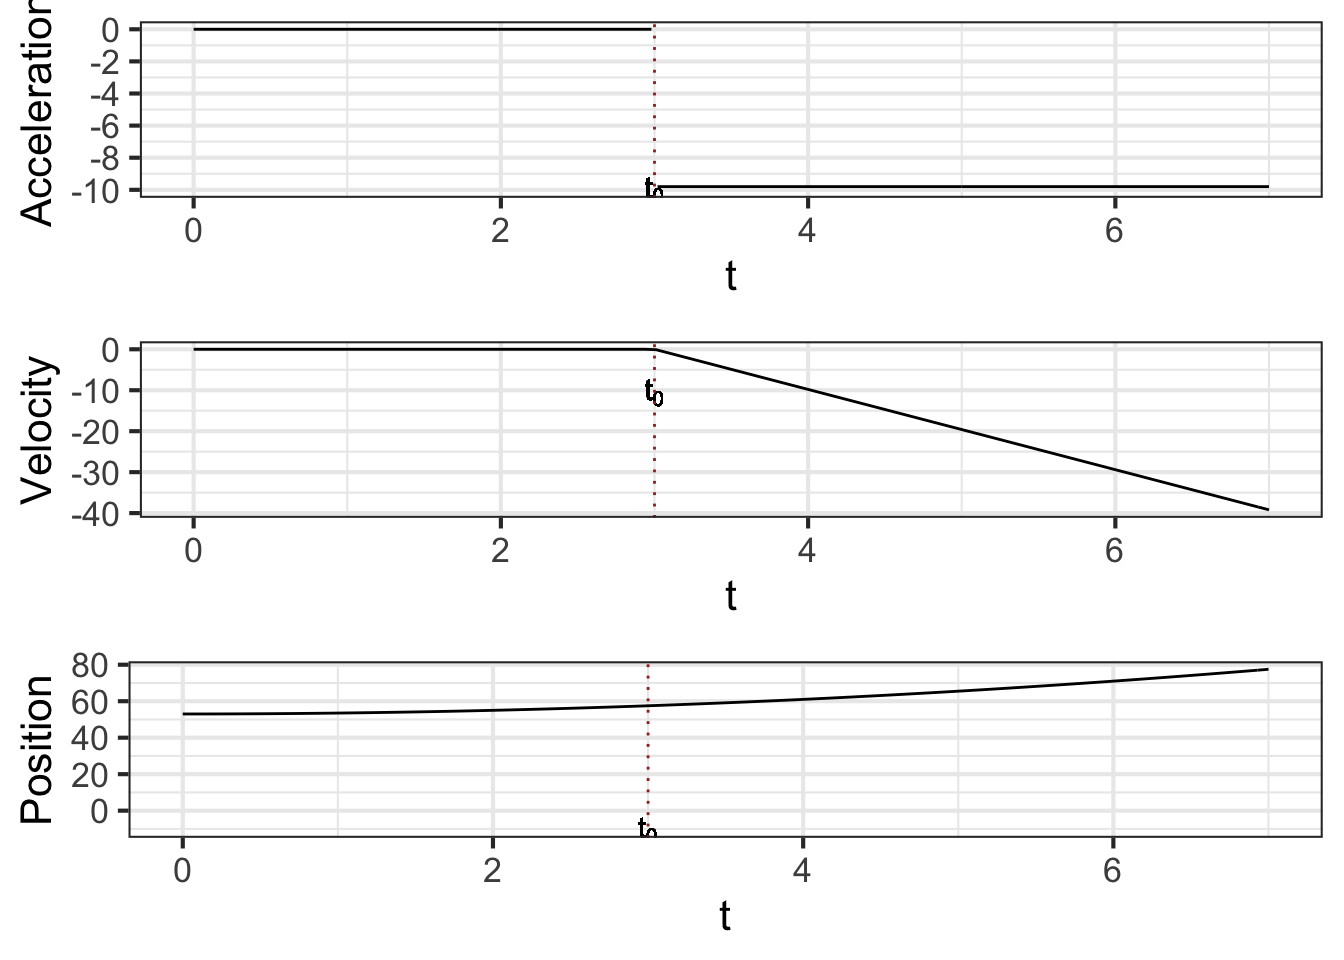
\includegraphics[width=0.9\textwidth,height=\textheight]{Accumulation/29-integration_files/figure-pdf/fig-galileo-accel-1.pdf}

}

\caption{\label{fig-galileo-accel}The acceleration, velocity, and
position of the ball as a function of time in Galileo's Tower of Pisa
experiment. The ball is released at time \(t_0\).}

\end{figure}

In the (fictional) account of the 1690 experiment, we had Galileo
release the ball at time \(t=0\). That's a common device in mathematical
derivations, but in a physical sense it's entirely arbitrary. Galileo
might have let go of the ball at any other time, say, \(t=3\) or
\(t=14:32:05\).

A remarkable feature of integrals is that it doesn't matter what we use
as the lower bound of integration, so long as we set the initial value
to correspond to that bound.

For a while you were writing integrals like this: \(\int_a^b f(t) dt\).
Then you replaced \(b\) with the input name \(t\) to get
\(\int_a^t f(t) dt\). But then you switched everything up by writing
\(\int_a^t f(x) dx\). Is that the same as \(\int_a^t f(t) dt\)? If so,
why do you get to replace the \(t\) with \(x\) in some places but not in
others?

Recall from Chapter 5 that the names used for inputs to a function
definition don't matter so long as they are used consistently on the
left and right sides of \(\equiv\). For instance, all these are the same
function:

\begin{itemize}
\tightlist
\item
  \(f(x) \equiv m x + b\)
\item
  \(g(t) \equiv m t + b\)
\item
  \(h(\text{wind}) \equiv m \text{wind} + b\)
\end{itemize}

Now think about the integral \(\int_a^b f(t) dt\):
\[\int_a^b f(t) dt = F(b) - F(a)\ .\]

On the left-hand side, the input name \(t\) is prominant, appearing in
two places: \(f(\color{magenta}{t}) d\color{magenta}{t}\). But \(t\) is
nowhere on the right-hand side. We could have equally well written this
as \(\int_a^b f(x) dx\) or \(\int_a^b f(\text{wind}) d\text{wind}\). The
name we use for the input to \(f()\) doesn't matter so long as it is
consistent with the name used in the \(d\_\_\) part of the notation.
Often, the name placed in the blanks in \(\int f(\_\_) d\_\_\) is called
a \textbf{\emph{dummy variable}}.

Writing \(\int_a^t f(t) dt\) is perfectly reasonable, but many authors
dislike the multiple appearance of \(t\). So they write something like
\(\int_a^t f(x) dx\) instead.

\hypertarget{integrals-from-bottom-to-top}{%
\section{Integrals from bottom to
top}\label{integrals-from-bottom-to-top}}

The bounds of integration appear in different arrangements. None of
these are difficult to derive from the basic forms:

\begin{itemize}
\tightlist
\item
  The relationship between an integral and its corresponding
  anti-derivative function: \[\int_a^b f(x) dx = F(b) - F(a)\] This
  relationship has a fancy-sounding name: the \textbf{\emph{second
  fundamental theorem of calculus}}.
\item
  The accumulation from an initial-value
  \[{\mathbf F}(b)\  =\  {\mathbf F}(a) + \int_a^b f(x) dx\  = \ {\mathbf F}(a) + F(b) - F(a)\]
  For many modeling situations, \(a\) and \(b\) are fixed quantities, so
  \(F(a)\) and \(F(b)\) are also quantities; the output of the
  anti-derivative function at inputs \(a\) and \(b\). But either the
  lower-bound or the upper-bound can be input names, as in
  \[\int_0^t f(x) dx = F(t) - F(0)\]
\end{itemize}

Note that \(F(t)\) is not a quantity but a function of \(t\).

On occasion, you will see forms like \(\int_t^0 f(x)dx\). You can think
of this in either of two ways:

\begin{enumerate}
\def\labelenumi{\arabic{enumi}.}
\tightlist
\item
  The accumulation from a time \(t\) less than 0 up until 0.
\item
  The \emph{reverse} accumulation from 0 until time \(t\).
\end{enumerate}

Reverse accumulation can be a tricky concept because it violates
everyday intuition. Suppose you were harvesting a row of ripe
strawberries. You start at the beginning of the row---position zero.
Then you move down the row, picking strawberries and placing them in
your basket. When you have reached position \(B\) your basket holds the
accumulation \(\int_0^B s(x)\, dx\), where \(s(x)\) is the lineal
density of strawberries---units: berries per meter of row.

But suppose you go the other way, starting with an empty basket at
position \(B\) and working your way back to position 0. Common sense
says your basket will fill to the same amount as in the forward
direction, and indeed this is the case. But integrals work differently.
The integral \(\int_B^0 s(x) dx\) will be the \textbf{negative} of
\(\int_0^B s(x) dx\). You can see this from the relationship between the
integral and the anti-derivative:
\[\int_B^0 s(x) dx \ = \ S(0) - S(B) \ =\ -\left[{\large\strut}S(B) - S(0)\right]\ = \ -\int_0^B s(x) dx\]

This is not to say that there is such a thing as a negative strawberry.
Rather, it means that harvesting strawberries is similar to an integral
in some ways (accumulation) but not in other ways. In farming,
harvesting from 0 to \(B\) is much the same as harvesting from \(B\) to
0, but integrals don't work this way.

Another property of integrals is that the interval between bounds of
integration can be broken into pieces. For instance:

\[\int_a^c f(x) dx \ = \ \int_a^b f(x) dx + \int_b^c f(x) dx\] You can
confirm this by noting that
\[\int_a^b f(x) dx + \int_b^c f(x) dx \ = \ \left[{\large\strut}F(b) - F(a)\right] + \left[{\large\strut}F(c) - F(b)\right] = F(c) - F(a) \ = \ \int_a^c f(x) dx\ .\]

Finally, consider this function of \(t\):
\[\partial_t \int_a^t f(x) dx\ .\] First, how do we know it is a
function of \(t\)? \(\int_a^t f(x) dx\) is a definite integral and has
the value \[\int_a^t f(x) dx = F(t) - F(a)\  .\] Following our
convention, \(a\) is a parameter and stands for a specific numerical
value, so \(F(a)\) is the output of \(F()\) for a specific input. But
according to convention \(t\) is the name of an input. So \(F(t)\) is a
function whose output depends on \(t\). Differentiating the function
\(F(t)\), as with every other function, produces a new function.

Second, there is a shortcut for calculating
\(\partial_t \int_a^t f(x) dx\):
\[\partial_t \int_a^t f(x) dx\ =\ \partial_t \left[{\large\strut}F(t) - F(a)\right]\ .\]
Since \(F(a)\) is a quantity and not a function,
\(\partial_t F(a) = 0\). That simplies things. Even better, we know that
the derivative of \(F(t)\) is simply \(f(t)\): that's just the nature of
the derivative/anti-derivative relationship between \(f(t)\) and
\(F(t)\). Put together, we have:
\[\partial_t \int_a^t f(x) dx\ =\ f(t)\ .\]

This complicated-looking identity has a fancy name: the
\textbf{\emph{first fundamental theorem of calculus}}.

Backtracking the stars.

In the 1920s, astronomers and cosmologists questioned the idea that the
large-scale universe is static and unchanging. This traditional belief
was undermined both by theory (e.g.~General Relativity) and
observations. The most famous of these were collected and published by
Edwin Hubble, starting in 1929 and continuing over the next decade as
improved techniques and larger telescopes became available. In recent
years, with the availability of the space telescope named in honor of
Hubble data has expanded in availability and quality.
Figure~\ref{fig-hubble-curve} shows a version of
\href{https://www.pnas.org/content/15/3/168}{Hubble's 1929 graph} based
on
\href{https://www.ncbi.nlm.nih.gov/pmc/articles/PMC314128/}{contemporary
data}.

\begin{figure}

{\centering 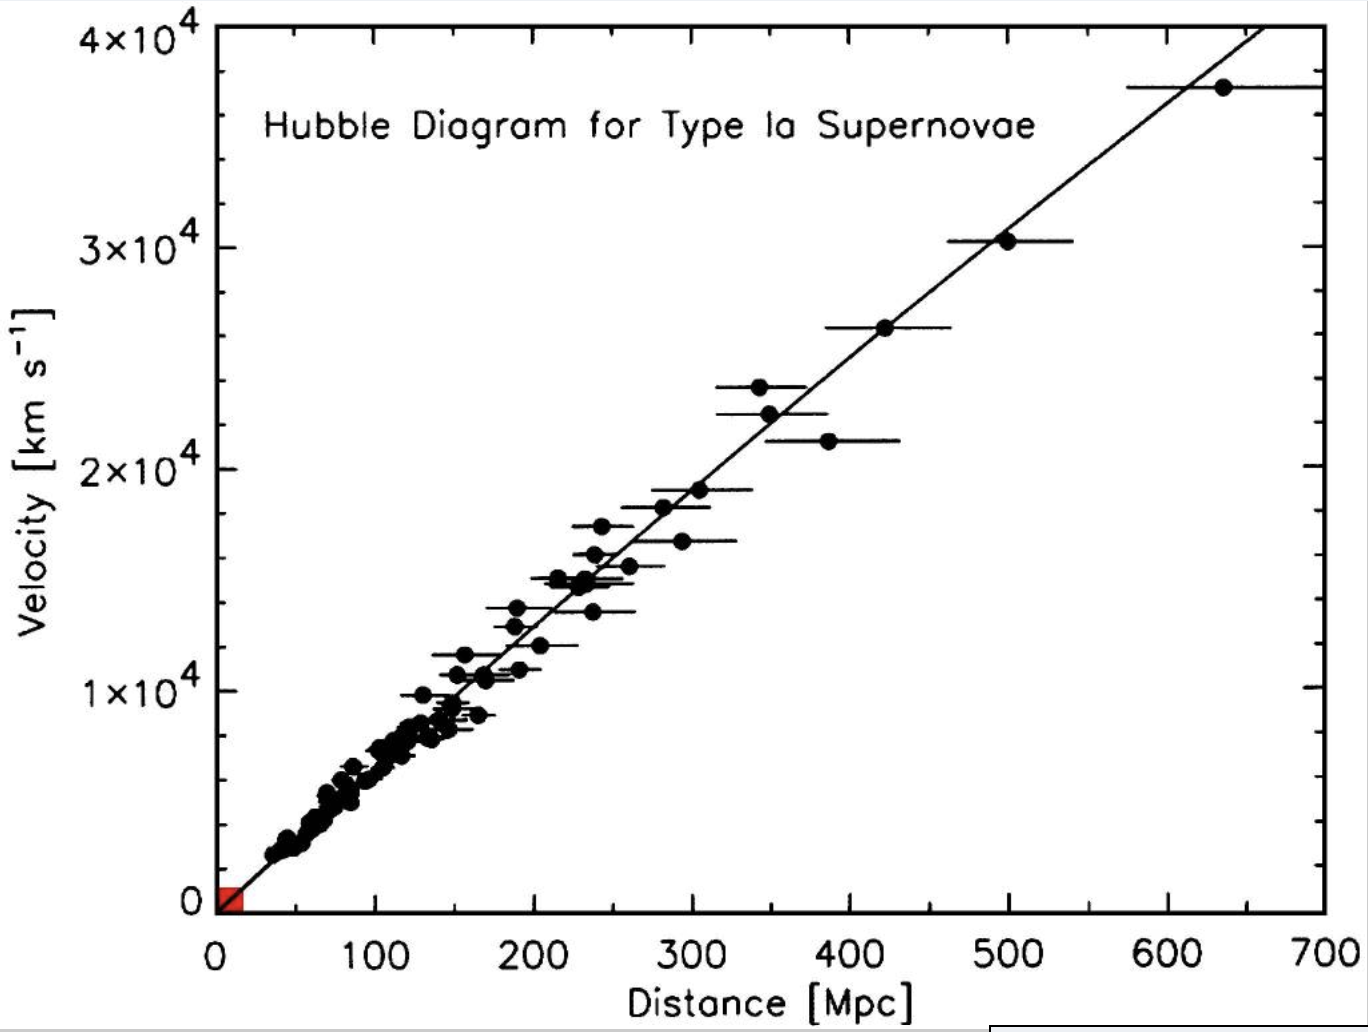
\includegraphics[width=0.6\textwidth,height=\textheight]{Accumulation/www/hubble-curve.png}

}

\caption{\label{fig-hubble-curve}The relationship between velocity and
distance of stars, using contemporary data in the same format at Edwin
Hubble's 1929 publication.}

\end{figure}

Each dot in Figure~\ref{fig-hubble-curve} is an exploding star called a
\emph{supernova}. The graph shows the relationship between the distance
of the star from our galaxy and the outward velocity of that star. The
velocities are large, \(3 \times 10^4 = 30,000\) km/s is about one-tenth
the speed of light. Similarly, the distances are big; 600 Mpc is the
same as 2 billion light years or \(1.8 \times 10^{22} \text{km}\). The
slope of the line in Figure~\ref{fig-hubble-curve} is
\(\frac{3.75 \times 10^4\, \text{km/s}}{1.8 \times 10^{22}\, \text{km}} = 2.1 \times 10^{-18}\, \text{s}^{-1}\).
For ease of reading, we'll call this slope \(\alpha\) and therefore the
velocity of a start distance \(D\) from Earth is
\[v(D) \equiv \alpha D\ .\]

Earlier in the history of the universe each star was a different
distance from Earth. We'll call this function \(D(t)\), distance as a
function of time in the universe.

The distance travelled by each star from time \(t\) (billions of years
ago) to the present is
\[\int_t^\text{now} v(t) dt  = D_\text{now} - D(t)\] which can be
re-arranged to give
\[D(t) = D_\text{now} - \int_t^\text{now} v(t) dt .\] Assuming that
\(v(t)\) for each star has remained constant at \(\alpha D_\text{now}\),
the distance travelled by each star since time \(t\) depends on it's
current distance like this:
\[\int_t^\text{now} v(t) dt = \int_t^\text{now} \left[ \alpha D_\text{now}\right]\, dt = \alpha D_\text{now}\left[\text{now} - t\right]\]
Thus, the position of each star at time \(t\) is
\[D(t) = D_\text{now} - \alpha D_\text{now}\left[\text{now} - t\right] = D(t)\]
or,
\[D(t) = D_\text{now}\left({\large\strut} 1-\alpha \left[\text{now} - t\right]\right)\]

According to this model, there was a common time \(t_0\) when when all
the stars were at the same place: \(D(t_0) = 0\). This happened when
\[\text{now} - t_0 = \frac{1}{\alpha} = \frac{1}{2.1 \times 10^{-18}\, \text{s}^{-1}} = 4.8 \times 10^{17} \text{s}\ .\]
It seems fair to call such a time, when all the stars where at the same
place at the same time, as the origin of the universe. If so,
\(\text{now} - t_0\) corresponds to the \textbf{\emph{age of the
universe}} and our estimate of that age is
\(4.8\times 10^{17}\text{s}\). Conventionally, this age is reported in
years. To get that, we multiply by the \textbf{\emph{flavor of one}}
that turns seconds into years:
\[\frac{60\, \text{seconds}}{1\, \text{minute}} \cdot \frac{60\, \text{minutes}}{1\, \text{hour}} \cdot \frac{24\, \text{hours}}{1\, \text{day}} \cdot \frac{365\, \text{days}}{1\, \text{year}} = 31,500,000 \frac{\text{s}}{\text{year}}\]
The grand (but hypothetical) meeting of the stars therefore occurred
\(4.8 \times 10^{17} \text{s} / 3.15 \times 10^{7} \text{s/year} = 15,000,000,000\)
years ago. Pretty crowded to have all the mass in the universe in one
place at the same time. No wonder they call it the Big Bang!

\hypertarget{exercises-2}{%
\section{Exercises}\label{exercises-2}}

\hypertarget{integrals-step-by-step}{%
\chapter{Integrals step-by-step}\label{integrals-step-by-step}}

The setting for anti-differentiation (and it's close cousin,
integration) is that we have a function \(F(t)\) which we do not yet
know, but we do have access to some information about it: its slope as a
function of time \(f(t) \equiv \partial_t F(t)\) and, perhaps, its value
\(F(t_0)\) at some definite input value.

Section~\ref{sec-totaling-bits} showed some ways to visualize the
construction of an \(F(t)\) by accumulating short segments of slope. The
idea is that we know \(f(t)\) which tells us, at any instant, the slope
of \(F(t)\). So, in drawing a graph of \(F(t)\), we put our pen to paper
at some input value \(t_0\) and then move forward in \(t\), setting the
instantaneous slope of our curve according to \(f(t)\).

In Section~\ref{sec-net-change}, we dealt with one of the limitations of
finding \(F(t)\) by anti-differentiation of \(f(t)\); the
anti-derivative is not unique. This is because to start drawing \(F(t)\)
we need pick a \(t_0\) and an initial value of \(F(t_0)\). If we had
picked a a different starting point \(t_1\) or a different initial value
\(F(t_1)\), the new curve would be different than the one drawn through
\((t_0, F(t_0))\), although it would have the same shape, just shifted
up or down according to our choice. We summarize this situation
algebraically by writing \[\int f(t) dt = F(t) + C\ ,\] where \(C\) is
the \textbf{\emph{constant of integration}}, that is, the vertical shift
of the curve.

The non-uniqueness of \(F(t)\) does not invalidate its usefulness. In
particular, the quantity \(F(b) - F(a)\), will be the same regardless of
which starting point we used to draw \(F(t)\). We have two names for
\(F(b) - F(a)\)

\begin{enumerate}
\def\labelenumi{\arabic{enumi}.}
\tightlist
\item
  The \textbf{\emph{net change}} in \(F()\) from \(a\) to \(b\).
\item
  The \textbf{\emph{definite integral}} of \(f()\) from \(a\) to \(b\),
  written \(\int_a^b f(t) dt\).
\end{enumerate}

These two things, the net change and the definite integral, are really
one and the same, a fact we describe by writing
\[\int_a^b f(t) dt = F(b) - F(a)\ .\]

In this chapter, we'll introduce a simple numerical method for
calculating from \(f()\) the net change/definite integral. This will be
a matter of trivial but tedious arithmetic: adding up lots of little
bits of \(f(t)\). Later, in Section~\ref{sec-accum-symbolic}, we'll see
how to avoid the tedious arithmetic by use of algebraic, symbolic
transformations. This symbolic approach has great advantages, and is the
dominant method of anti-differentiation found in college-level science
textbooks. However, there are many common \(f(t)\) for which the
symbolic approach is not possible, whereas the numerical method works
for any \(f(t)\). Even more important, the numerical technique has a
simple natural extension to some commonly encountered accumulation
problems that look superficially like they can be solved by
anti-differentiation but rarely can be in practice. We'll meet one such
problem and solve it numerically, but a broad approach to the topic,
called \textbf{\emph{dynamics}} or \textbf{\emph{differential
equations}}, will have to wait until Block 6.

\hypertarget{euler-method}{%
\section{Euler method}\label{euler-method}}

The starting point for this method is the definition of the derivative
of \(F(t)\). Reaching back to Chapter 8,

\[\partial_t F(t) \equiv \lim_{h\rightarrow 0} \frac{F(t+h) - F(t)}{h}\]
To translate this into a numerical method for computing \(F(t)\), let's
write things a little differently.

\begin{itemize}
\tightlist
\item
  First, since the problem setting is that we don't (yet) know \(F(t)\),
  let's refer to things we do know. In particular, we know
  \(f(t) = \partial_t F(t)\).
\item
  Again, recognizing that we don't yet know \(F(t)\), let's re-write the
  expression using something that we do know: \(F(t_0)\). Stated more
  precisely, \(F(t_0)\) is something we get to make up to suit our
  convenience. (A common choice is \(F(t_0)=0\).)
\item
  Let's replace the symbol \(h\) with the symbol \(dt\). Both of them
  mean ``a little bit of'' and \(dt\) makes explicit that we mean ``a
  little bit of \(t\).''
\item
  We'll substitute the limit \(\lim_{h\rightarrow 0}\) with an
  understanding that \(dt\) will be something ``small.'' How small?
  We'll deal with that question when we have to tools to answer it.
\end{itemize}

With these changes, we have
\[f(t_0) = \frac{F(t_0+dt) - F(t_0)}{dt}\ .\] The one quantity in this
relationship that we do not yet know is \(F(t_0 + dt)\). So re-arrange
the equation so that we can calculate the unknown in terms of the known.
\[F(t_0 + dt) = F(t_0) + f(t_0)\, dt\ .\]

Let's consider finding the anti-derivative of \(\dnorm()\), that is,
\(\int_0^t \dnorm(x) dx\). In one sense, you already know the answer,
since \(\partial_x \pnorm(x) = \dnorm(x)\). In reality, however, we know
\(\pnorm()\) only because it has been numerically constructed by
integrating \(\dnorm()\). The \(\pnorm()\) function is so important that
the numerically constructed answer has been memorized by software.

\hypertarget{area}{%
\section{Area}\label{area}}

The quantity \[\Large \color{magenta}{f(t_0)}\, \color{orange}{dt}\]
gives rise to a visualization that has been learned by generations of
calculus students. The visualization is so compelling and powerful that
many students (and teachers, and textbook authors) mistake the
visualization for integration and anti-differentiation themselves.

We'll start the visualization with a simple graph of \(f(t)\), which is
called the \textbf{\emph{integrand}} in the integral
\(\int_a^b f(t) dt\). Figure~\ref{fig-area-integrand} shows the graph of
\(f(t)\). A specific point \(t_0\) has been marked on the horizontal
axis. Next to it is another mark at \(t_0 + dt\). Of course, the
distance between these marks is \(\color{orange}{dt}\).

\begin{figure}

\sidecaption{\label{fig-area-integrand}Illustrating the interpretation
of \(f(t_0) dt\) as an ``area''.}

{\centering 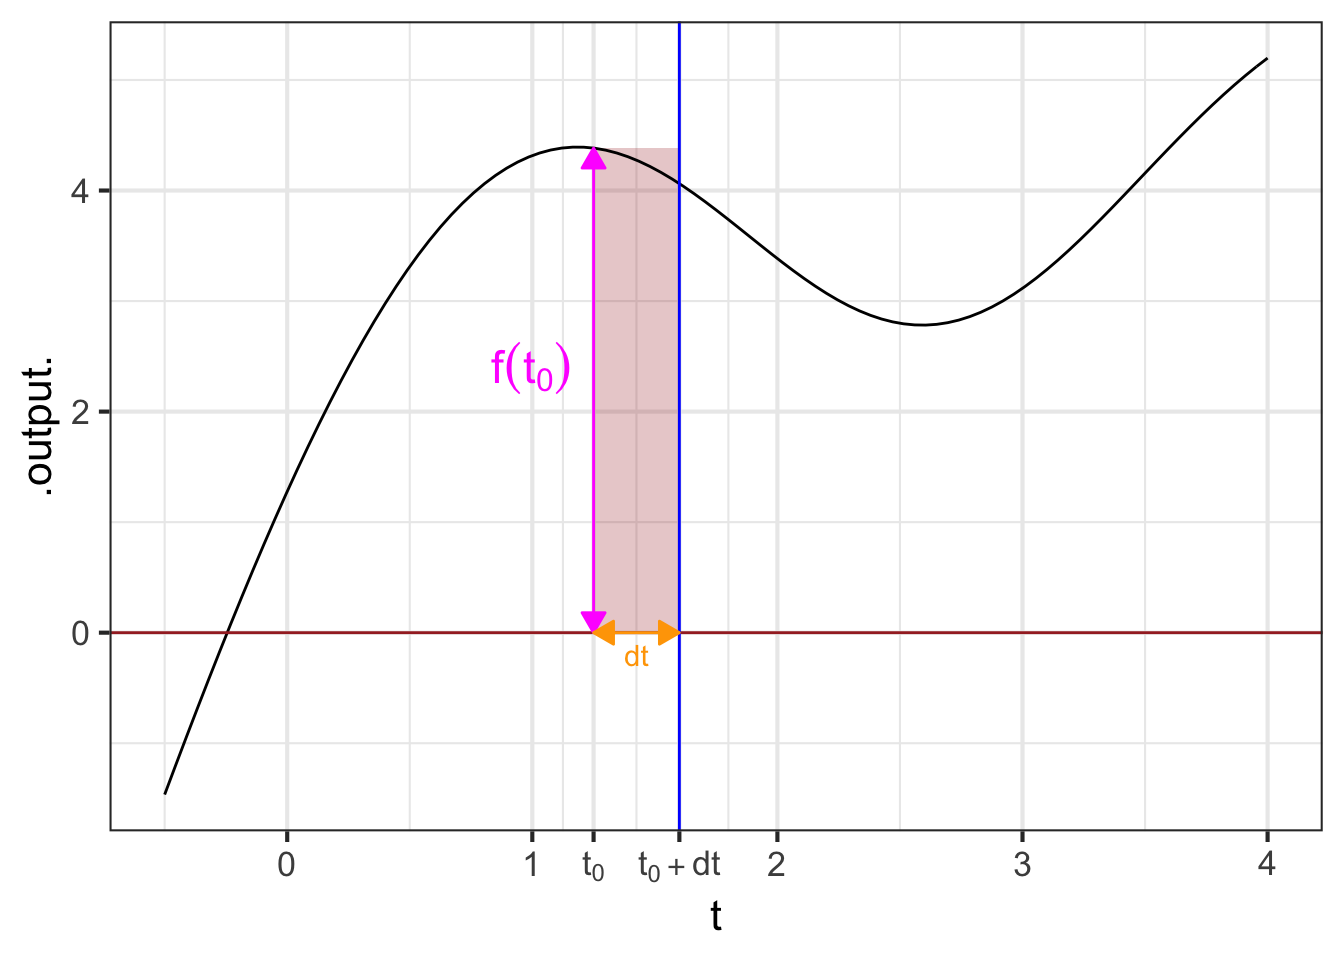
\includegraphics[width=0.9\textwidth,height=\textheight]{Accumulation/30-euler_files/figure-pdf/fig-area-integrand-1.pdf}

}

\end{figure}

Per the usual graphical convention, a position along the vertical axis
corresponds to a possible output of \(f(t)\). The output for \(t=t_0\)
is \(\color{magenta}{f(t_0)}\). That same quantity corresponds to the
length of the vertical orange segment connecting \((t_0, 0)\) to
\((t_0, f(t_0))\).

The \(\color{orange}{dt}\) line segment and the
\(\color{magenta}{f(t_0)}\) segment constitute two sides of a rectangle,
shown as a shaded zone. The ``area'' of that rectangle is the product
\(\color{magenta}{f(t_0)}\ \color{orange}{dt}\).

In this sort of visualization, an integral is the accumulation of many
of these \(f(t) dt\) rectangles. For instance, Figure~\ref{fig-bars-0-3}
the visualization of the integral \[\int_{0}^3 f(t) dt\ .\]

\begin{verbatim}
## Warning in is.na(x): is.na() applied to non-(list or vector) of type
## 'expression'

## Warning in is.na(x): is.na() applied to non-(list or vector) of type
## 'expression'

## Warning in is.na(x): is.na() applied to non-(list or vector) of type
## 'expression'
\end{verbatim}

\begin{figure}

\sidecaption{\label{fig-bars-0-3}Visualizing the integral
\(\int_0^3 f(t) dt\) as the total ``area'' of several \(f(t) dt\) bars.
The width of each of the bars is \(dt\). The height depends on the value
of the function \(f(t)\) at the bar. For illustration, two of the bars
are marked with vertical and horizontal line segments.}

{\centering 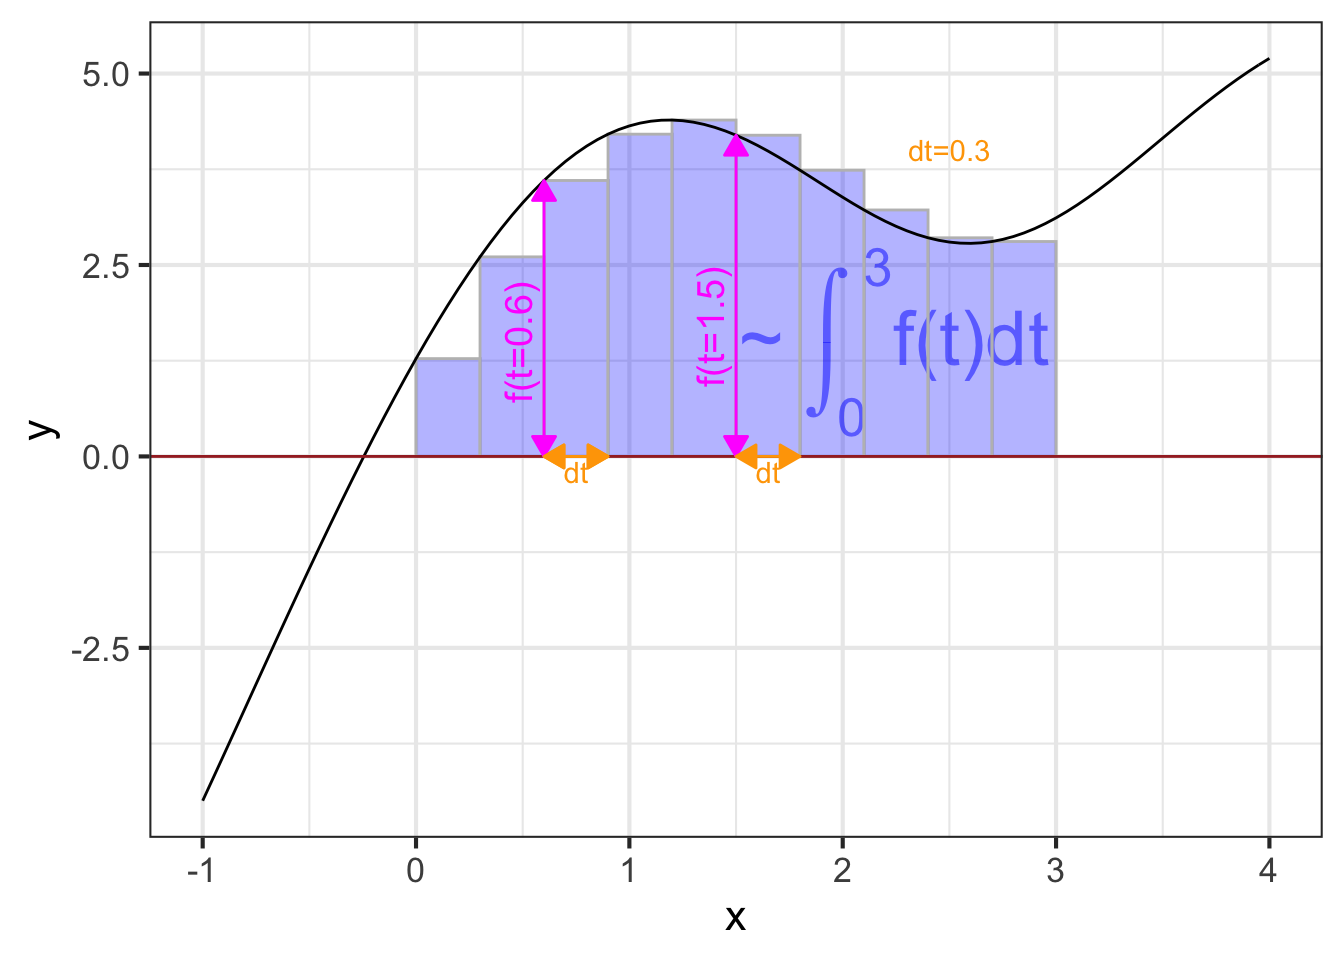
\includegraphics[width=0.9\textwidth,height=\textheight]{Accumulation/30-euler_files/figure-pdf/fig-bars-0-3-1.pdf}

}

\end{figure}

As always in calculus, we imagine \(dt\) as a ``small'' quantity. In
\textbf{?@fig-bars-0-3b} you can see that the function output changes
substantially over the sub-domain spanned by a single rectangle. Using
smaller and smaller \(dt\), as in \textbf{?@fig-bars-0-3-small} brings
the visualization closer and closer to the actual meaning of an
anti-derivative.

\begin{figure}

\sidecaption{Visualizing the integral \(\int_0^3 f(t) dt\) as the total
``area'' of several \(f(t) dt\) bars. The width of each of the bars is
\(dt\). The height depends on the value of the function \(f(t)\) at the
bar. For illustration, two of the bars are marked with vertical and
horizontal line segments.}

{\centering 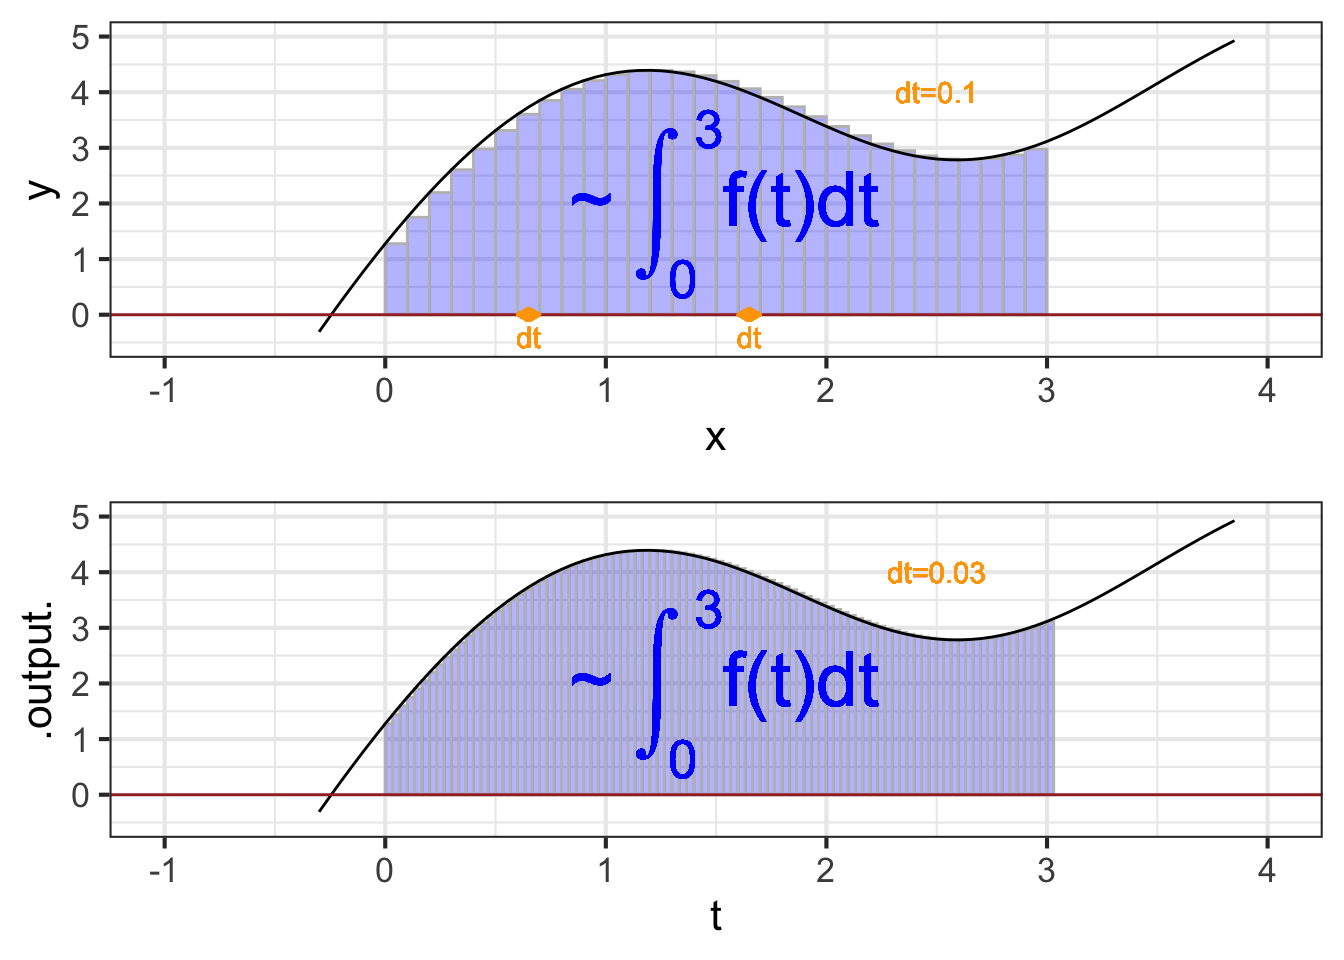
\includegraphics[width=0.9\textwidth,height=\textheight]{Accumulation/30-euler_files/figure-pdf/bars-0-3B-1.pdf}

}

\end{figure}

\begin{why}
Why do you keep putting ``area'' in quotes?

When \(f(t_i) < 0\), then \(f(t_i) dt\) will be negative. There is no
such thing as a negative area, but in constructing an integral the
\(f(t_i)dt\), being negative, diminishes the accumulated area.

\begin{figure}

{\centering 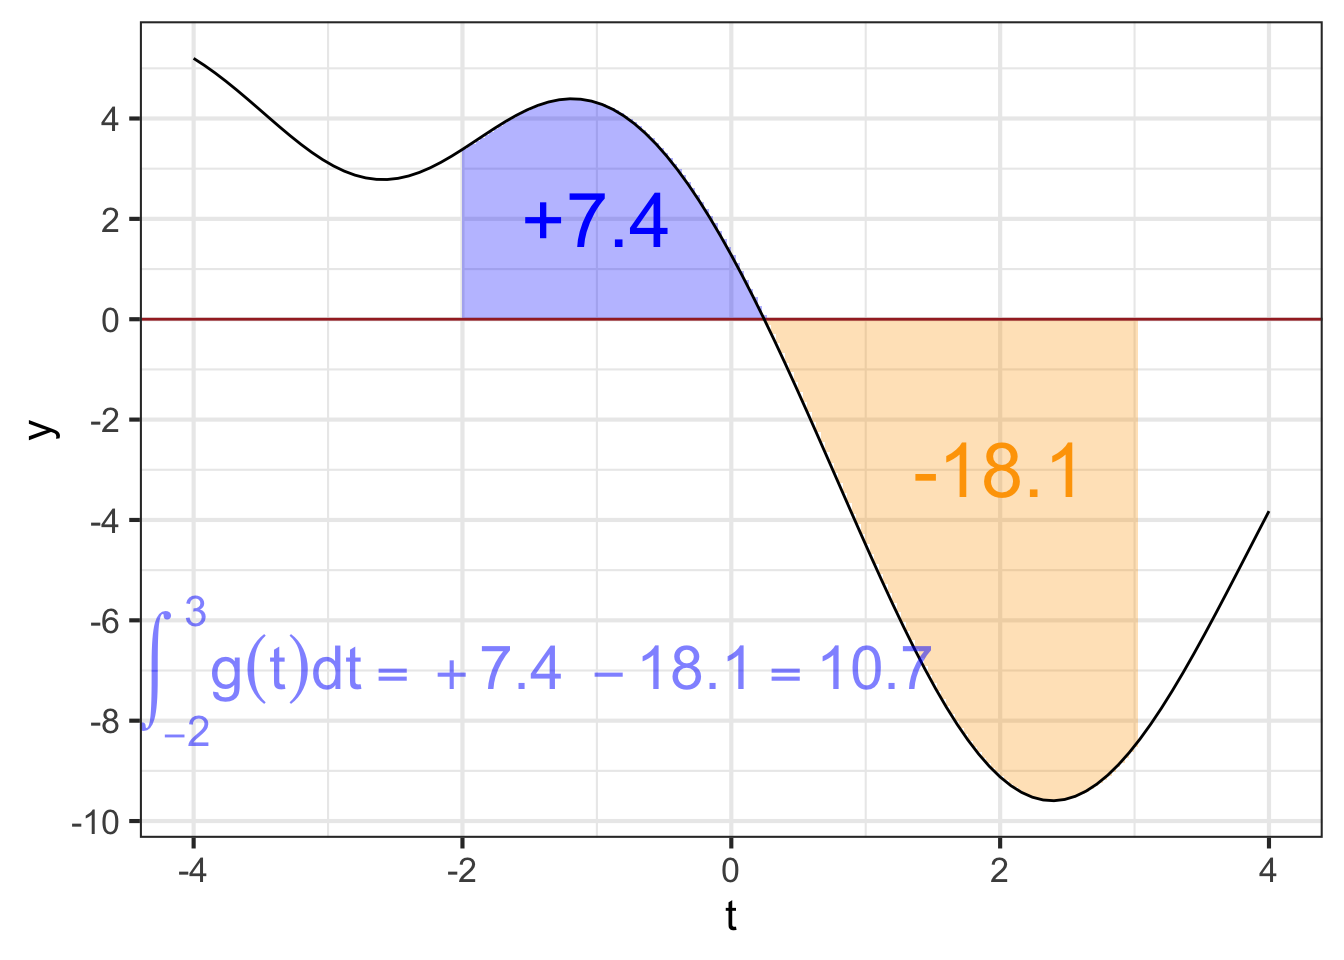
\includegraphics[width=0.9\textwidth,height=\textheight]{Accumulation/30-euler_files/figure-pdf/fig-neg-area-1.pdf}

}

\caption{\label{fig-neg-area}The \(\int_{-2}^3 g(t) dt\) covers
subdomains where \(g(t) > 0\) and where \(g(t) < 0\). In those latter
subdomains, the ``area'' is negative, and shown in light orange here.}

\end{figure}

Another problem is that area is a physical quantity, with dimension
L\(^2\). The quantity produced by integration will have physical
dimension \([f(t)][t]\), the product of the dimension of the
with-respect-to quantity and the output of the function.

``Area'' is an effective metaphor for visualizing integration, but the
goal of integration is not to calculate an area but, typically, some
other kind of quantity.

\end{why}

\hypertarget{the-euler-step}{%
\section{The Euler Step}\label{the-euler-step}}

The previous section a visualization of an integral in terms of an area
on a graph. As you know, a definite integral \(\int_a^b f(t) dt\) can
also be computed by constructing the anti-derivative
\(F(t) \equiv \int f(t) dt\) and evaluating it at the upper and lower
bounds of integration: \(F(b) - F(a)\). In this section, we'll look at
the numerical process of constructing an anti-derivative function, which
uses many of the same concepts as those involved in finding an integral
by combining areas of rectangles.

A definite integral produces a \textbf{quantity}, not a function. The
anti-derivative function constructed by using quantities like
\(f(t) dt\) will be a \textbf{\emph{series of quantities}} rather than a
formula. In particular, it will have the form of a data table, something
like this:

\marginnote{\begin{footnotesize}

\begin{longtable}[]{@{}ll@{}}
\toprule
\(t\) & \(F(t)\) \\
\midrule
\endhead
-2 & 10.62 \\
-1.5 & 6.47 \\
-1 & 3.51 \\
-0.5 & 2.02 \\
0 & 2.4 \\
0.5 & 3.18 \\
1.0 & 5.14 \\
\(\vdots\) & \(\vdots\) \\
\bottomrule
\end{longtable}

\end{footnotesize}}

To start, we'll need to create a series of \(t\) values. We'll do this
by specifying a starting value for \(t\) and then creating successive
values by adding a numerical increment \(dt\) to the entries one after
the other until we reach a terminating value. For instance, in the above
table, the starting value for \(t\) is \(-2\), the numerical increment
is \(dt=0.5\), and the terminating value is \(1\).

In previous chapters of this book we have worked with data tables, but
always the data table was \emph{given} to us, we did not have to
construct it.\sidenote{\footnotesize The root of the word ``data'' is the Latin for
  ``given''.} Now we need to construct the data frame with the \(t\)
column containing appropriate values. Computer languages provide many
ways to accomplish this task. We'll use a simple R/mosaic function
\texttt{Picket()}, which constructs a data table like the one shown
above. You provide two arguments: the domain for \(t\), that is, the
desired upper and lower bounds of integration; the interval size \(dt\)
(which is called \texttt{h} in the argument list). For instance, to
construct the \(t\) column of the table shown above, you can use
\texttt{Picket()} this way:

\begin{Shaded}
\begin{Highlighting}[]
\NormalTok{Pts }\OtherTok{\textless{}{-}} \FunctionTok{Picket}\NormalTok{(}\FunctionTok{domain}\NormalTok{(}\AttributeTok{t =} \SpecialCharTok{{-}}\DecValTok{2}\SpecialCharTok{:}\DecValTok{1}\NormalTok{), }\AttributeTok{h=}\FloatTok{0.5}\NormalTok{)}
\NormalTok{Pts}
\DocumentationTok{\#\# \# A tibble: 6 x 3}
\DocumentationTok{\#\#       t preweight weight}
\DocumentationTok{\#\#   \textless{}dbl\textgreater{}     \textless{}dbl\textgreater{}  \textless{}dbl\textgreater{}}
\DocumentationTok{\#\# 1  {-}2           1    0.5}
\DocumentationTok{\#\# 2  {-}1.5         1    0.5}
\DocumentationTok{\#\# 3  {-}1           1    0.5}
\DocumentationTok{\#\# 4  {-}0.5         1    0.5}
\DocumentationTok{\#\# 5   0           1    0.5}
\DocumentationTok{\#\# 6   0.5         1    0.5}
\end{Highlighting}
\end{Shaded}

As you can see, the data table produced by \texttt{Picket()} has the
\(t\) column, as well as a second column named \texttt{weight}. We
haven't explained \texttt{weight} yet, but you can see that it is the
same value we specified as \texttt{h}.

The name \texttt{Picket()} is motivated by the shape of a picket fence.
The pickets are evenly spaced, which keeps things simple but is not a
requirement.

Note that the picket does not say anything at all about the function
\(f(t)\) being anti-differentiated. The picket can be applied to any
function although precision might require a smaller \(dt\) for functions
that have a lot going on in a small domain.

The next step in using the picket to perform anti-differentiation is to
apply the function \(f()\) to the pickets. That is, we'll add a new
column, perhaps called \texttt{vals} to the data table.

Adding a new column is a common task when dealing with data. We'll do
this with a new function, \texttt{mutate()}, whose specific function is
adding new columns (or modifying old ones). Here's the command to apply
\(f()\) to \texttt{t} and call the new column \texttt{vals}:

\begin{Shaded}
\begin{Highlighting}[]
\CommentTok{\# Find the height of the pickets}
\NormalTok{Pts }\OtherTok{\textless{}{-}}\NormalTok{ Pts }\SpecialCharTok{\%\textgreater{}\%}
  \FunctionTok{mutate}\NormalTok{(}\AttributeTok{vals =} \FunctionTok{f}\NormalTok{(t))}
\end{Highlighting}
\end{Shaded}

With this modification, the data table looks like:

\begin{verbatim}
## # A tibble: 6 x 4
##       t preweight weight  vals
##   <dbl>     <dbl>  <dbl> <dbl>
## 1  -2           1    0.5 -9.12
## 2  -1.5         1    0.5 -7.27
## 3  -1           1    0.5 -4.50
## 4  -0.5         1    0.5 -1.46
## 5   0           1    0.5  1.28
## 6   0.5         1    0.5  3.31
\end{verbatim}

Now that we know the value of the function at each of the pickets, the
next step is to multiply the value by the spacing between pickets. That
spacing, which we set with the argument \texttt{h\ =\ 0.5} in our
original call to \texttt{Picket()} is in the column called
\texttt{weight}. We'll call the result of the multiplication
\texttt{step}. Note that the following R command incorporates the
previous calculation of \texttt{vals}; we're looking to build up a
single command that will do all the work.

\begin{Shaded}
\begin{Highlighting}[]
\CommentTok{\# Multiply the height by the picket spacing}
\NormalTok{Pts }\OtherTok{\textless{}{-}}\NormalTok{ Pts }\SpecialCharTok{\%\textgreater{}\%}
  \FunctionTok{mutate}\NormalTok{(}\AttributeTok{vals =} \FunctionTok{f}\NormalTok{(t),}
         \AttributeTok{step =}\NormalTok{ vals }\SpecialCharTok{*}\NormalTok{ weight)}
\end{Highlighting}
\end{Shaded}

\begin{Shaded}
\begin{Highlighting}[]
\NormalTok{Pts}
\DocumentationTok{\#\# \# A tibble: 6 x 5}
\DocumentationTok{\#\#       t preweight weight  vals   step}
\DocumentationTok{\#\#   \textless{}dbl\textgreater{}     \textless{}dbl\textgreater{}  \textless{}dbl\textgreater{} \textless{}dbl\textgreater{}  \textless{}dbl\textgreater{}}
\DocumentationTok{\#\# 1  {-}2           1    0.5 {-}9.12 {-}4.56 }
\DocumentationTok{\#\# 2  {-}1.5         1    0.5 {-}7.27 {-}3.63 }
\DocumentationTok{\#\# 3  {-}1           1    0.5 {-}4.50 {-}2.25 }
\DocumentationTok{\#\# 4  {-}0.5         1    0.5 {-}1.46 {-}0.732}
\DocumentationTok{\#\# 5   0           1    0.5  1.28  0.639}
\DocumentationTok{\#\# 6   0.5         1    0.5  3.31  1.66}
\end{Highlighting}
\end{Shaded}

We used the name \texttt{step} to identify the product of the height and
spacing of the pickets to help you think about the overall calculation
as accumulating a series of steps. Each step provides a little more
information about the anti-derivative that we will now calculate. In
terms of the area metaphor for integration, each step is the area of one
vertical bar of the sort presented in the previous section.

We'll call these \textbf{\emph{Euler steps}}, a term that will be
especially appropriate when, in Block 6, we use integration to calculate
the trajectories of systems---such as a ball in flight---that change in
time.

The final step in constructing the anti-derivative is to add up the
steps. This is simple addition. But we'll arrange the addition one step
at a time. That is, for the second row, the result will be the sum of
the first \emph{two} steps. For the third row, the result will be the
sum of the first \emph{three} steps. And so on. The name for this sort
of accumulation of the previous steps is called a
\textbf{\emph{cumulative sum}}. Another name for a cumulative sum is a
``running sum'': the sum-so-far as we move down the column of steps.
Cumulative sums are computed in R by using \texttt{cumsum()}. Here,
we're calling the result of the cumulative sum \texttt{F} to emphasize
that it is the result of anti-differentiating \(f()\). But keep in mind
that the anti-derivative is not just the \texttt{F} column, but the
table with both \texttt{t} and \texttt{F} columns. That is, the table
has a column for the input as well as the output. That's what it takes
to be a function.

\begin{Shaded}
\begin{Highlighting}[]
\CommentTok{\# Doing everything in one command}
\NormalTok{Pts }\OtherTok{\textless{}{-}} 
  \FunctionTok{Picket}\NormalTok{(}\FunctionTok{domain}\NormalTok{(}\AttributeTok{t =} \SpecialCharTok{{-}}\DecValTok{2}\SpecialCharTok{:}\DecValTok{1}\NormalTok{), }\AttributeTok{h=}\FloatTok{0.5}\NormalTok{) }\SpecialCharTok{\%\textgreater{}\%}
  \FunctionTok{mutate}\NormalTok{(}\AttributeTok{vals =} \FunctionTok{f}\NormalTok{(t),}
         \AttributeTok{step =}\NormalTok{ vals }\SpecialCharTok{*}\NormalTok{ weight,}
         \AttributeTok{F =} \FunctionTok{cumsum}\NormalTok{(step))}
\end{Highlighting}
\end{Shaded}

\begin{verbatim}
## # A tibble: 6 x 6
##       t preweight weight  vals   step      F
##   <dbl>     <dbl>  <dbl> <dbl>  <dbl>  <dbl>
## 1  -2           1    0.5 -9.12 -4.56   -4.56
## 2  -1.5         1    0.5 -7.27 -3.63   -8.19
## 3  -1           1    0.5 -4.50 -2.25  -10.4 
## 4  -0.5         1    0.5 -1.46 -0.732 -11.2 
## 5   0           1    0.5  1.28  0.639 -10.5 
## 6   0.5         1    0.5  3.31  1.66   -8.88
\end{verbatim}

We can summarize the steps in this Euler approach to numerical
integration graphically:

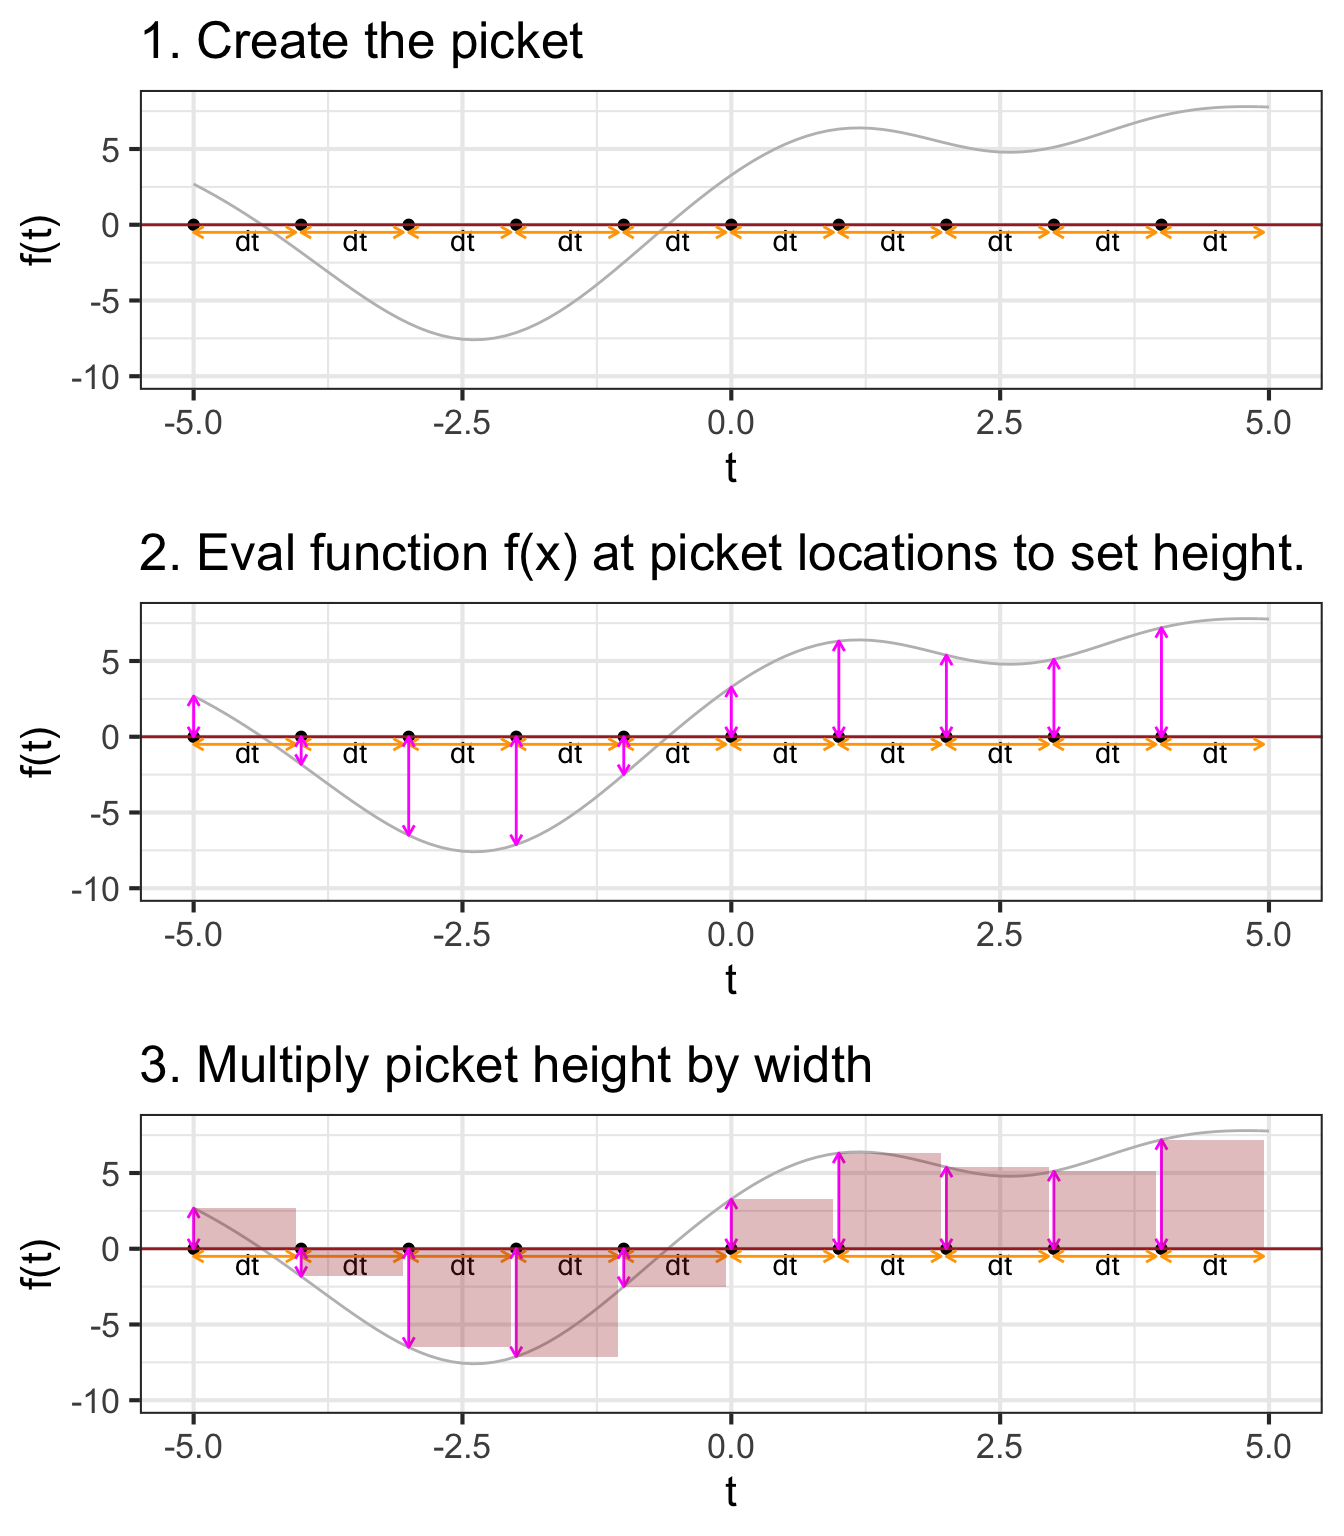
\includegraphics{Accumulation/30-euler_files/figure-pdf/fig-euler-integration1,-1.pdf}\{\#fig-euler-integration1,
fig-align=`center' width=90\%\}

\begin{figure}

{\centering 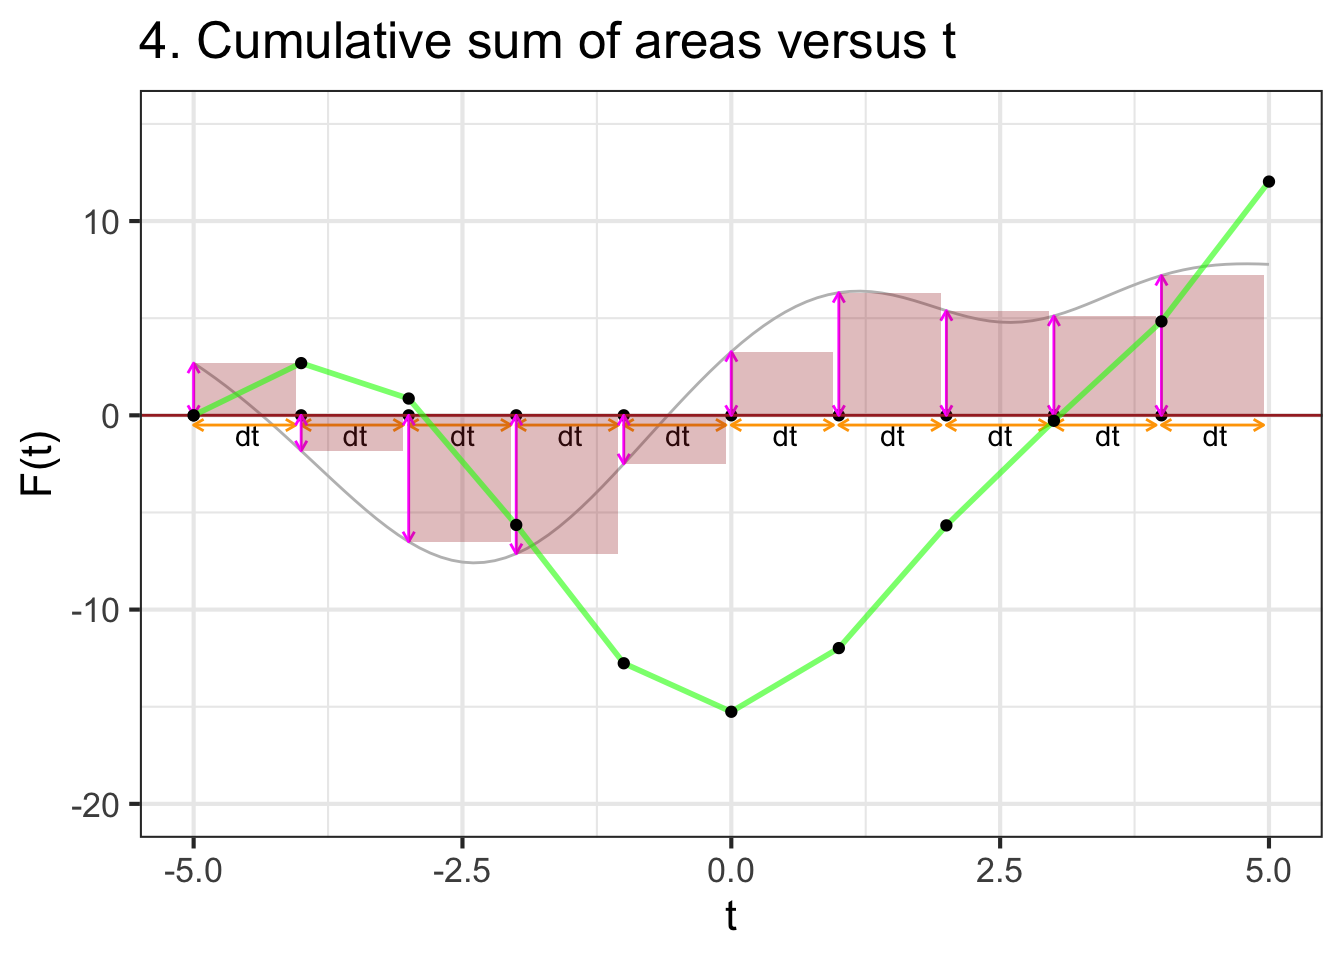
\includegraphics[width=0.9\textwidth,height=\textheight]{Accumulation/30-euler_files/figure-pdf/fig-euler-integration2-1.pdf}

}

\caption{\label{fig-euler-integration2}Steps in a numerical construction
of an anti-derivative. (1) Create a set of picket locations over the
domain of interest. The locations are spread horizontally by amount dt,
so each picket will be dt units wide. (2) evaluate the original function
at the picket points to give picket heights. (3) Multiply the picket
height by the picket width to create an ``area''. (4) Starting at zero
for the left-most picket, add in successive picket areas to construct
the points on the anti-derivative function (green). Note that the
vertical axis in (4) has a different dimension and units than in steps
(1)-(3). In (4) the vertical scale is in the units of the
anti-derivative function output.}

\end{figure}

Figure~\ref{fig-dynamic-anti-d} shows a dynamic version of the process
of constructing an anti-derivative by Euler steps. The integrand
\(f(t)\) is shown in the top panel, the anti-derivative \(F(t)\) is
shown being built up in the bottom panel. The
\(\color{magenta}{\text{magenta}}\) bar in the top plot is the current
Euler step. That step is added to the previously accumulated steps to
construct \(F(t)\).

PROVIDE LINK TO MOVIE IN PDF version.

\begin{figure}

{\centering 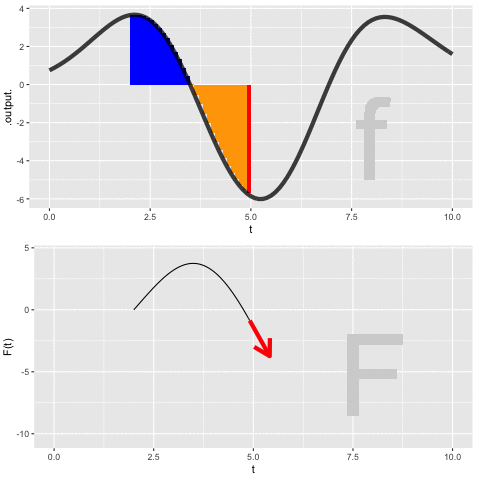
\includegraphics[width=0.9\textwidth,height=\textheight]{Accumulation/www/area-plot-still.png}

}

\caption{\label{fig-dynamic-anti-d}A dynamic view of building \(F(t)\)
from \(f(t)\) by accumulating Euler steps.}

\end{figure}

\begin{intheworld}
The following graphic from a well-respected news magazine,
\emph{\href{https://www.economist.com/img/b/600/653/90/sites/default/files/images/print-edition/20210710_EUC776.png}{The
Economist}}, shows the reported number of cases and deaths from Covid-19
during a two-year period in Russia. (``Sputnik'' is the name given to a
Russian-developed vaccine, named after the
\href{https://en.wikipedia.org/wiki/Sputnik_1}{first man-made satellite}
in Earth orbit, launched by the Soviet Union on Oct.~4, 1957 and
precipitating a Cold-War crisis of confidence in in the US.)

\begin{figure}

{\centering 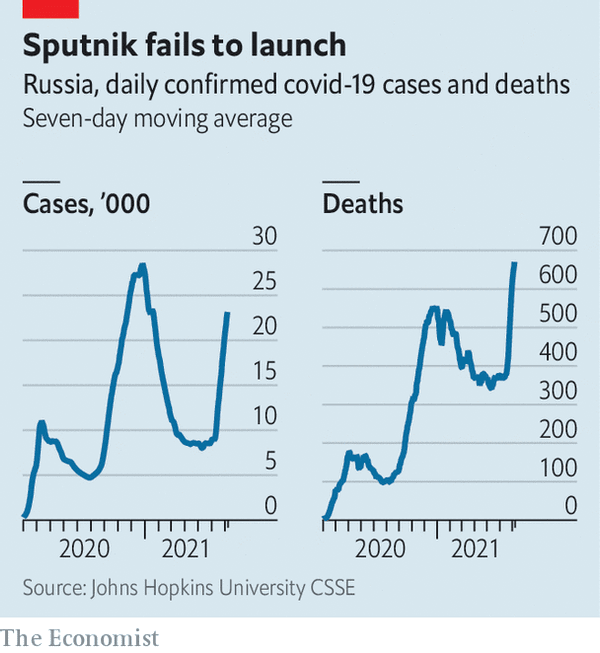
\includegraphics[width=0.9\textwidth,height=\textheight]{Accumulation/www/sputnik.png}

}

\end{figure}

The figure caption gives information about the units of the quantities
being graphed. Notice the word ``daily,'' which tells us, for example,
that in mid-2021 there were about 10,000 new cases of Covid-19 each day
and correspondingly about 350 daily deaths.

How many total cases and total deaths are reported in the graphic?

There are, of course, two distinct ways to present such data which can
be easily confused by the casual reader. One important way to present
data is as \textbf{\emph{cumulative}} cases and deaths as a function of
date. We'll call these \(C(t)\) and \(D(t)\). Another prefectly
legitimate presentation is of the rate of change \(\partial_t C(t)\) and
\(\partial_t D(t)\) which, following our informal
capital/lower-case-letter convention, we could write \(c(t)\) and
\(d(t)\). Since there is no such thing as a ``negative'' case or death,
we know that \(C(t)\) and \(D(t)\) are monotonic functions, never
decreasing. So the graphs cannot possibly be of \(C(t)\) and \(D(t)\),
since the graphs are far from monotonic. Consequently, the displayed
graphs are \(c(t)\) and \(d(t)\), as confirmed by the word ``daily'' in
the caption.

To find \(C(t)\) and \(D(t)\) requires integrating \(c(t)\) and
\(d(t)\). The value of \(C(t)\) and \(D(t)\) at the right-most extreme
of the graph can be found by calculating the ``area'' under the \(c(t)\)
and \(d(t)\) curves. But care needs to be taken in reading the
horizontal axis. Although the axes are labelled with the year, the tick
marks are spaced by one month. (Notice ``month'' does not appear in the
caption.) The far right end of the graph is in early July 2021. The far
left end, when the graph moves away from zero cases and deaths, is early
April 2020.

You can do a reasonable job estimating the ``area'' by extending the
tick marks on the horizontal axis and counting the resulting rectangles
that fall under the curve.

\begin{figure}

{\centering \includegraphics[width=0.9\textwidth,height=\textheight]{Accumulation/www/sputnik-bars.png}

}

\end{figure}

For the graph of cases, the ``area'' of each rectangle is
\(\frac{5000\, \text{cases}}{\text{ day}}\cdot \text{1 month}\). This
has the right dimension, ``cases,'' but the units are screwy. So replace
1 month with 30.5 days (or thereabouts) to get an ``area'' of each
rectangle of 172,500 cases. Similarly, the ``area'' of the rectangles on
the right graph is 3050 deaths.

\end{intheworld}

\hypertarget{better-numerics-optional}{%
\section{Better numerics (optional)}\label{better-numerics-optional}}

Except as a textbook exercise, you will likely never have to compute a
numerical anti-derivative from scratch as we did in the previous
section. This is a good thing. To understand why, you have to know one
of the important features of modern technical work. That feature is: We
never work alone in technical matters. There is always a set of people
whose previous work we are building on, even if we never know the names
of those people. This is because technology is complicated and it is
evidently beyond the reach of any human to master all the salient
aspects of each piece of technology being incorporated into the work we
consider our own.

Of course this is true for computers, since no individual can build a
useful computer from first principles. It's also true for software. One
detail in particular is relevant to us here. Computer arithmetic of the
sort used in the previous section---particularly addition---is prone to
error when adding up lots and lots of small bits. This means that it is
not always sensible to choose very small \(dt\) in order to get a very
accurate approximation to the anti-derivative.

Fortunately, there are specialists in numerical mathematics who work on
ways to improve the accuracy of calculations for mid-sized \(dt\). Their
work has been incorporated into the results of \texttt{antiD()} and
\texttt{Integrate()} and so the details are, for us, unimportant. But
they are only unimportant because they have been taken care of.

To illustrate how considerably more accuracy can be gained in
calculating an anti-derivative, consider that the rectangular bars drawn
in the previous sections are intended to approximate the ``area'' under
the function. With this in mind, we can replace the rectangular bars
with more suitable shapes that stay closer to the function over the
finite extend of each \(dt\) domain. The rectangular bars model the
function as piecewise constant. A better job can be done with piecewise
linear approximations or piecewise quadratic approximations. Often, such
refinements can be implemented merely by changing the weight column in
the picket data frame used to start off the process.

One widely used method, called \textbf{\emph{Gauss-Legendre quadrature}}
can calculate a large segment of an integral accurately (under
conditions that are common in practice) with just five evaluations of
the integrand \(f(t)\).

\begin{margintable}

\caption{Picket locations and weights For the integral
\(\int_a^b f(t) dt\) where \(c = \frac{a+b}{2}\) and
\(w = (b-a)/2\).}\begin{minipage}[t]{\linewidth}

{\centering 

\begin{longtable}[]{@{}ll@{}}
\toprule
location & weight \\
\midrule
\endhead
\(c - 0.90618 w\) & \(0.236927 \times w\) \\
\(c - 0.53847 w\) & \(0.478629 \times w\) \\
\(c\) & \(0.568889 \times w\) \\
\(c + 0.53847 w\) & \(0.478629 \times w\) \\
\(c + 0.90618 w\) & \(0.236927 \times w\) \\
\bottomrule
\end{longtable}

}

\end{minipage}%

\end{margintable}

The locations and weights may seem like a wizard parody of mathematics,
but those precise values are founded in an advanced formulation of
polynomials rooted in the theory of linear combinations to which you'll
be introduced in Block 5. Needless to say, you can hardly be expected to
have any idea where they come from. That's why it's useful to build on
the work of experts in specialized areas. It's particularly helpful when
such expertise is incorporated into software that faithfully and
reliably implements the methods. The lesson to take to heart: Use
professional software systems that have been extensively vetted.

\hypertarget{exercises-3}{%
\section{Exercises}\label{exercises-3}}

\hypertarget{sec-accum-symbolic}{%
\chapter{Symbolic anti-differentiation}\label{sec-accum-symbolic}}

You have already learned how to write down, by sight, the
anti-derivative of the many of the pattern-book functions. As a
reminder, here is an (almost) complete list of the derivatives and
anti-derivatives of the pattern-book functions.

\begin{longtable}[]{@{}
  >{\raggedright\arraybackslash}p{(\columnwidth - 4\tabcolsep) * \real{0.3600}}
  >{\raggedright\arraybackslash}p{(\columnwidth - 4\tabcolsep) * \real{0.3400}}
  >{\raggedright\arraybackslash}p{(\columnwidth - 4\tabcolsep) * \real{0.3000}}@{}}
\toprule
\begin{minipage}[b]{\linewidth}\raggedright
\(\partial_x f(x)\)
\end{minipage} & \begin{minipage}[b]{\linewidth}\raggedright
\(f(x)\)
\end{minipage} & \begin{minipage}[b]{\linewidth}\raggedright
\(\int f(x) dx\)
\end{minipage} \\
\midrule
\endhead
\(e^x\) & \(e^x\) & \(e^x\) \\
\(\cos(x)\) & \(\sin(x)\) & \(-\cos(x)\) \\
\(p x^{p-1}\) & power-law \(x^p\) & \(\frac{1}{p+1} x^{p+1}\) \\
\(\ \ \ \ 2x\) & \(\ \ \ \ x^2\) & \(\frac{1}{3} x^3\) \\
\(\ \ \ \ 1\) & \(\ \ \ \ x\) & \(\frac{1}{2} x^2\) \\
\(\ \ \ \ 0\) & \(\ \ \ \ 1\) & \(x\) \\
\(\ \ \ \ -x^{-2}\) & \(\ \ \ \ 1/x\) & \(\ln(|x|)\) \\
\(1/x\) & \(\ln(x)\) & \(x \left(\strut\ln(x) - 1\right)\) \\
\(-x \dnorm(x)\) & \(\dnorm(x)\) & \(\pnorm()\) \\
\(\dnorm(x)\) & \(\pnorm(x)\) & See below. \\
\bottomrule
\end{longtable}

You can see that the derivatives and anti-derivatives of the
pattern-book functions can be written in terms of the pattern-book
functions. The left column contains the \textbf{\emph{symbolic
derivatives}} of the pattern book functions.\sidenote{\footnotesize One small
  deviation from the pattern-book functions is
  \(\int \frac{dx}{x} = \ln(|x|)\). The absolute value \(|x|\) in
  \(\ln(|x|)\) reflects the differing domains of the functions
  \(\ln(x)\) and \(1/x\). Logarithms are defined only the positive half
  of the number line, while the reciprocal function \(1/x\) is defined
  for all non-zero \(x\). Including the absolute value in the argument
  to log covers situations such as \(\int_{-2}^{-1} \frac{dx}{x}\) which
  has the value \(\ln(2)\).} The right column contains the
\textbf{\emph{symbolic anti-derivatives}}. We call them ``symbolic,''
because they are written down with the same kind of symbols that we use
for writing the pattern-book functions themselves.\sidenote{\footnotesize Mathematicians
  have a list that is a bit longer than our pattern-book
  functions---they call them \textbf{\emph{elementary functions}} and
  include the tangent and other trig functions and their inverses, as
  well as what are called ``hyperbolic functions'' and their inverses.}

We're stretching things a bit by including \(\dnorm(x)\) and
\(\pnorm(x)\) among the functions that can be integrated symbolically.
As you'll see later, \(\dnorm(x)\) is special when it comes to
integration.

Think of the above table as the ``basic facts'' of differentiation and
anti-differentiation. It's well worth memorizing the table since it
shows many of the relationships among the functions that are central to
this book. For the sinusoids, we've used the traditional name
\(\cos(x)\) to refer to \(\sin(x + \pi/2)\) and \(-\cos(x)\) instead of
\(\sin(x - \pi/2)\) since generations of calculus students have been
taught to name ``cosine'' as the derivative of ``sine,'' and don't
always remember the relationship that \(\cos(x) =\sin(x + \pi/2)\).

For differentiation, any function that can be written using combinations
of the pattern-book functions by multiplication, composition, and linear
combination has a derivative that can be written using the pattern-book
functions. So a complete story of symbolic differentiation is told by
the above table and the differentiation rules:

\begin{itemize}
\item
  linear combination:
  \(\partial_x \left[{\strut}a\, f(x) + b\, g(x)\right] = a\, \partial_x f(x) + b\, \partial_x g(x)\)
\item
  product:
  \(\partial_x \left[{\strut}f(x)\cdot g(x)\right] = g(x) \partial_x f(x) + f(x) \partial_x g(x)\)
\item
  composition:
  \(\partial_x \left[{\strut}f(g(x))\right] = \left[\partial_x f{\large\strut}\right]\!\left({\large\strut}g(x)\right) \cdot \partial_x g(x)\)
\end{itemize}

This chapter is about the analogous rules for anti-differentiation. The
anti-differentiation rule for linear combination is simple: essentially
the same as the rule for differentiation.

\[\int \left[\strut a\, f(x) + b\, g(x)\right] dx = a\!\int\! f(x) dx + b\!\int\! g(x) dx\]
How about the rules for function products and for composition? The
surprising answer is that there are \textbf{no such rules}. There is no
template analogous to the product and chain rules for derivatives, that
can consistently be used for anti-derivatives. What we have instead are
\textbf{\emph{techniques of integration}}, somewhat vague rules that
will sometimes guide a successful search for the anti-derivative, but
often will lead you astray.

Indeed, there are many functions for which a symbolic anti-derivative
cannot be constructed from compositions and/or multiplication of
pattern-book functions that can be written using pattern-book
functions.\sidenote{\footnotesize Again, mathematicians prefer to refer to the
  ``elementary functions'' rather than the pattern-book functions.
  \(\dnorm()\) and \(\pnorm()\) are not elementary functions, and there
  are several elementary function that we don't include in the
  pattern-book list.}

Fortunately, we already know the symbolic anti-derivative form of many
functions. We'll call those the \textbf{\emph{cataloged functions}}, but
this is not a term in general use in mathematics. For functions not in
the catalog, it is non-trivial to find out whether the function has a
symbolic anti-derivative or not. This is one reason why the techniques
of integration do not always provide a result.

The following sections provide an overview of techniques of integration.
We start with a description of the cataloged functions and direct you to
computer-based systems for looking up the catalog. (These are almost
always faster and more reliable than trying to do things by hand.) Then
we introduce a new interpretation of the notation for
anti-differentiation: differentials. This interpretation makes it
somewhat easier to understand the major techniques of integration:
substitution and integration by parts. We'll finish by returning to a
setting where symbolic integration is easy: polynomials.

Remember that, even if we cannot always find a symbolic anti-derivative,
that we can always construct a numerical anti-derivative that will be
precise enough for almost any genuine purpose.

\hypertarget{sec-cataloged-functions}{%
\section{The cataloged functions}\label{sec-cataloged-functions}}

In a traditional science or mathematics education, students encounter
(almost exclusively) basic functions from a mid-sized catalog. For
instance: \(\sqrt{\strut\_\_\_\ }\), \(\sin()\), \(\cos()\), \(\tan()\),
square(), cube(), recip(), \(\ln()\), \(\exp()\), negate(), gaussian(),
and so on. This catalog also includes some functions that take two
arguments but are traditionally written without using parentheses. For
instance, \(a+b\) doesn't look like a function but is entirely
equivalent to \(+(a, b)\). Others in this class are \(\times(\ ,\ )\),
\(\div(\ , \ )\), \(-(\ ,\ )\), and \^{}( , ).

The professional applied mathematician's catalog is much larger. You can
see an example published by the US National Institute of Standards and
Technology as the \href{https://dlmf.nist.gov/}{Digital Library of
Mathematical Functions}. (Almost all of the 36 chapters in this catalog,
important though they be, are highly specialized and not of general
interest across fields.)

There is a considerable body of theory for these \textbf{\emph{cataloged
functions}}, which often takes the form of relating them to one another.
For instance, \(\ln(a \times b) = \ln(a) + \ln(b)\) demonstrates a
relationship among \(\ln()\), \(+\) and \(\times\). Along the same lines
of relating the cataloged functions to one another is
\(\partial_x \sin(x) = \cos(x)\) and other statements about derivatives
such as those listed in Chapter \textbf{?@sec-computing-derivs}.

Simply to illustrate what a function catalog looks like,
Figure~\ref{fig-table-of-integrals} shows a page from an 1899 handbook
entitled
\href{https://archive.org/details/integralstable00peirrich/page/114/mode/2up}{\emph{A
Short Table of Integrals}}.

\begin{marginfigure}

{\centering \includegraphics[width=0.9\textwidth,height=\textheight]{Accumulation/www/table-of-integrals-1.png}

}

\caption{\label{fig-table-of-integrals}Entries 124-135 from \emph{A
Short Table of Integrals} (1899) by Benjamin Osgood Pierce. The book
includes 938 such entries.}

\end{marginfigure}

The use of cataloged functions is particularly prevalent in textbooks,
so the quantitatively sophisticated student will encounter symbolic
anti-derivatives of these functions throughout his or her studies.

The cataloged functions were assembled with great effort by
mathematicians over the decades. The techniques and tricks they used to
find symbolic anti-derivatives are not part of the everyday experience
of technical workers, although many mathematically minded people find
them a good source of recreation.

Calculus textbooks that include extensive coverage of the techniques and
tricks should be understood as telling a story of the historical
construction of catalogs, rather than conveying skills that are widely
used today. In a practical sense, when the techniques are needed, it's
more reliable to access them via computer interface such as
WolframAlpha, as depicted in Figure~\ref{fig-wolfram-alpha-125}.

\begin{marginfigure}

{\centering 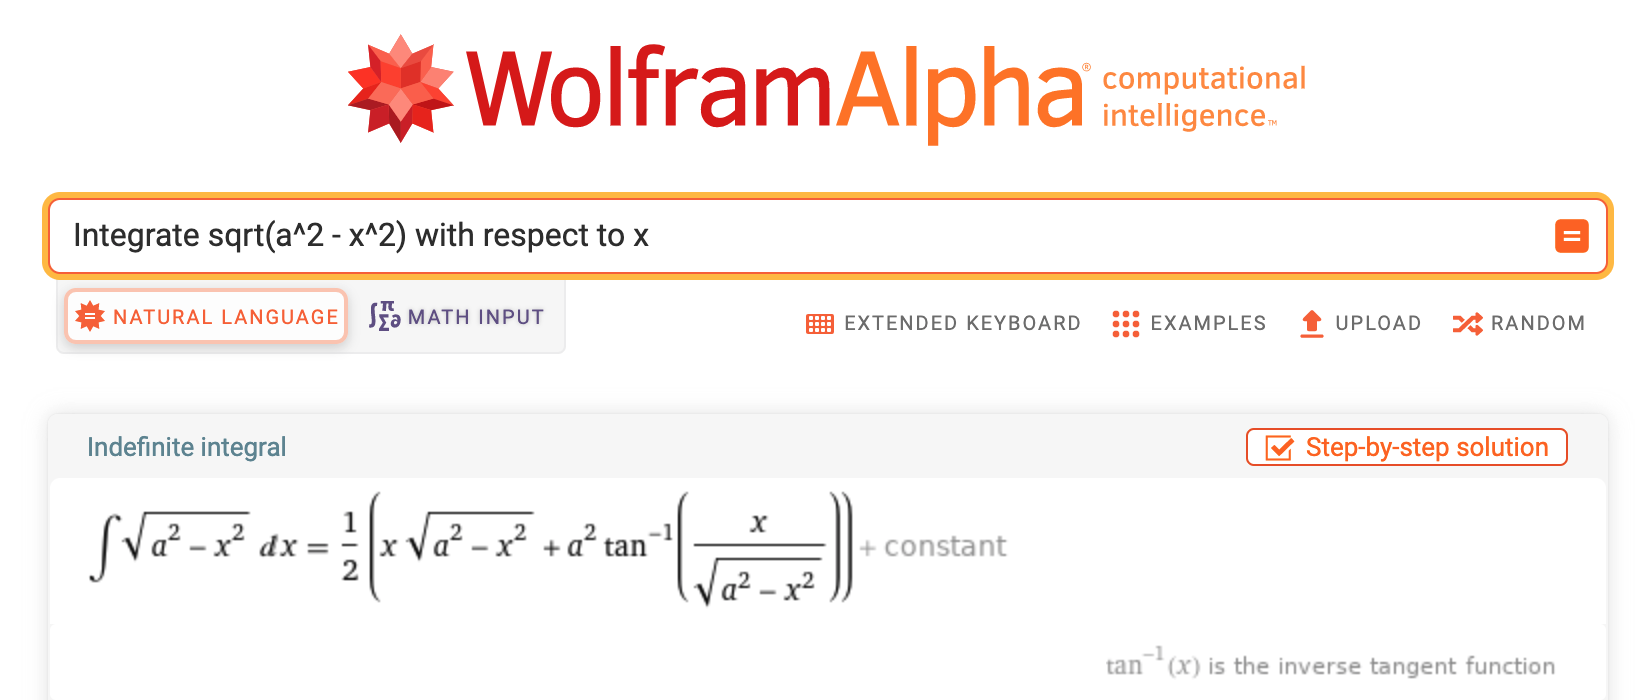
\includegraphics[width=0.9\textwidth,height=\textheight]{Accumulation/www/wolfram-alpha-125.png}

}

\caption{\label{fig-wolfram-alpha-125}Pierce's entry 125 as computed by
the WolframAlpha system.}

\end{marginfigure}

The systems can do a good job identifying cases where the techniques
will not work. In such systems, they provide the anti-derivative as
constructed by numerical integration. The R/mosaic \texttt{antiD()}
function works in this same way, although its catalog contains only a
tiny fraction of the functions found in professional systems. (But then,
only a tiny fraction of the professional cataloged function are widely
used in applied work.)

\hypertarget{differentials}{%
\section{Differentials}\label{differentials}}

Breathing some life into the symbol \(dx\) will help in understanding
the algebra of techniques for anti-differentiating function compositions
and products. We've thus far presented \(dx\) as a bit of notation:
punctuation for identifying the with-respect-to input in
anti-derivatives. That is, in interpreting a sequence of symbols like
\(\int f(x,t) dx\), we've parsed the sequence of symbols into three
parts:

\[\underbrace{\int}_{\text{integral sign}} \overbrace{f(x, t)}^{\text{function to be anti-differentiated}} \underbrace{dx}_{\text{'with respect to'}}\]

By analogy, the English sentence

\[\text{We loaded up on snacks.}\]

consists of five parts: the five words in the sentence.

But you can also see ``We loaded up on snacks'' as having \emph{three}
parts:

\[\underbrace{\text{We}}_{\text{subject}}\  
\overbrace{\text{loaded up on}}^{\text{verb}}\ \ \ 
\underbrace{\text{snacks}}_{\text{object}}\]

Likewise, the integrate sentence can be seen as consisting of just two
parts:

\[\underbrace{\int}_{\text{integral sign}} \overbrace{f(x, t) dx}^{\text{differential}}\]

A differential corresponds to the little sloped segments that we add up
when calculating a definite integral numerically using the
\textbf{\emph{slope function visualization}}. That is
\[\underbrace{\int}_{\text{Sum}} \underbrace{\overbrace{f(x,t)}^\text{slope of segment}\ \  \overbrace{dx}^\text{run}}_\text{rise}\]

A differential is a genuine mathematical object and is used, for
example, in analyzing the geometry of curved spaces, as in the Theory of
General Relativity. But this is well beyond the scope of this
introductory calculus course.

Our use here for differentials will be to express rules for
anti-differentiation of function compositions and products.

You should be thinking in terms of differentials when you see a sentence
like the following:

\begin{quote}
``In \(\int \sin(x) \cos(x) dx\), make the substitution \(u = \sin(x)\),
implying that \(du = \cos(x) dx\) and getting \(\int u du\), which is
simple to integrate.''
\end{quote}

The table gives some examples of functions and their differentials.
``w.r.t'' means ``with respect to.''

\begin{table*}

\caption{\textbf{?(caption)}}\begin{minipage}[t]{\linewidth}

{\centering 

\begin{longtable}[]{@{}
  >{\raggedright\arraybackslash}p{(\columnwidth - 6\tabcolsep) * \real{0.2500}}
  >{\raggedright\arraybackslash}p{(\columnwidth - 6\tabcolsep) * \real{0.3333}}
  >{\raggedright\arraybackslash}p{(\columnwidth - 6\tabcolsep) * \real{0.1389}}
  >{\raggedright\arraybackslash}p{(\columnwidth - 6\tabcolsep) * \real{0.2778}}@{}}
\toprule
\begin{minipage}[b]{\linewidth}\raggedright
Function
\end{minipage} & \begin{minipage}[b]{\linewidth}\raggedright
derivative
\end{minipage} & \begin{minipage}[b]{\linewidth}\raggedright
w.r.t.
\end{minipage} & \begin{minipage}[b]{\linewidth}\raggedright
differential
\end{minipage} \\
\midrule
\endhead
\(v(x) \equiv x\) & \(\partial_x v(x) = 1\) & x & \(dv = dx\) \\
\(u(x) \equiv x^2\) & \(\partial_x u(x) = 2x\) & x & \(du = 2x dx\) \\
\(f(x) \equiv \sin(x)\) & \(\partial_x f(x) = \cos(x)\) & x &
\(df = \cos(x)dx\) \\
\(u(x) \equiv e^{3 x}\) & \(\partial_x u(x) = 3 e^{3 x}\) & x &
\(du = 3 e^{3 x} dx\) \\
\(g(x) \equiv t^3\) & \(\partial_t v(t) = 3 t^2\) & t &
\(dg = 3 t^2 dt\) \\
\bottomrule
\end{longtable}

}

\end{minipage}%

\end{table*}

As you can see, the \emph{differential} of a function is simply the
derivative of that function followed by the little \(dx\) or \(dt\) or
whatever is appropriate for the ``with respect to'' input.

Notice that the differential of a function is not written with
parentheses: The function \(u(x)\) corresponds to the differential
\(du\).

\begin{example}
What is the differential of \(\sin(x)\)?

As we've seen, \(\partial_x \sin(x) = cos(x)\). For form the
differential of \(\sin()\), take the derivative and suffix it with a
\(dx\) (since \(x\) is the name of the input):

\[\cos(x)\ dx\]

\end{example}

\hypertarget{u-substitution}{%
\section{U-substitution}\label{u-substitution}}

There is little reason to use \(\partial_t\) and
\(\int \left[\right]dt\) to cancel each other out, but it is the basis
of an often successful strategy---\textbf{\emph{u-substitution}}---for
finding anti-derivatives symbolically. Here's the
differentiate/integrate algorithm behind u-substitution.

\begin{enumerate}
\def\labelenumi{\arabic{enumi}.}
\tightlist
\item
  Pick a function \(f()\) and another function \(g()\). Typically
  \(f()\) and \(g()\) belong to the family of basic modeling functions,
  e.g.~\(e^x\), \(\sin(t)\), \(x^n\), \(\ln(x)\), and so on. For the
  purpose of illustration, we'll use \(f(x) = \ln(x)\) and
  \(g(t) = \cos(t)\).
\item
  Compose \(f()\) with \(g()\) to produce a new function \(f(g())\)
  which, in our case, will be \(\ln(\cos(t))\).
\item
  Use the chain rule to find \(\partial_t f(g(t))\). In the example, the
  derivative of \(\ln(x)\) is \(1/x\), the derivative of \(g(t)\) is
  \(-\sin(t)\). By the chain rule,
  \[\partial_t f\left(\strut g(t)\right) = \partial_t \underbrace{\Large\ln}_{f()}\left(\underbrace{\large\cos(t)}_{g(t)}\right) = \underbrace{\left[- \frac{1}{\cos(t)}\right]}_{f'(g(t))} \underbrace{\left[{\LARGE\strut}\sin(t)\right]}_{g'(t)} = -  \frac{\sin(t)}{\cos(t)} = - \tan(t)\]
\end{enumerate}

In a sense, we have just watched a function give birth to another
through the straightforward process of differentiation. Having witnessed
the birth, we know who is the integration parent of \(\tan(t)\), namely
\(\int \tan(t) dt = \ln\left(\cos(t)\right)\). For future reference, we
might write this down in our diary of integrals:
\[\int \tan(t) dt = - \ln(\cos(t)) + C\] Saving this fact in your diary
is helpful. The next time you need to find \(\int \tan(x) dx\), you can
look up the answer (\(-\ln(\cos(x)) + C\)) from your diary. If you use
\(\int \tan(x) dx\) a lot, you will probably come to memorize the
answer, just as you have already memorized that
\(\int \cos(t) dt = \sin(t)\) (a fact that you will use a lot in the
rest of this course).

Now for the u-substitution game. The trick is to take a problem of the
form \(\int h(t) dt\) and extract from \(h(t)\) two functions, an
\(f()\) and a \(g()\). You're going to do this so that
\(h(t) = \partial_t F(g(t))\), where \(\partial_x F(x) = f(x)\) Once
you've done this, you have an answer to the original integration
question: \(\int h(t) dt = F(g(t)) + C\).

\begin{example}

Task: Evaluate the definite integral \(\int \frac{\sin(\ln(x))}{x} dx\).

You don't know ahead of time that this is an integral amenable to
solution by u-substitution. For all you know, it's not. So before you
start, look at the function to see if it one of those for which you
already know the anti-derivative, for example any of the pattern-book
functions or their parameterized cousins the basic modeling functions.

\begin{quote}
If so, you've already memorized the answer and you are done. If not
\ldots{}
\end{quote}

Assume for a moment---without any guarantee that this will work, mind
you---that the answer can be built using u-substitution. You will
therefore look hard at \(h()\) and try to see in it a plausible form
that looks like the derivative of some \(f(g(x))\).

In the problem at hand, we can readily see something of the form
\(f(g(x))\) in the \(\sin(\ln(x))\). This immediately gives you a
candidate for \(g(x)\), namely \(g(x)\equiv \ln(x)\) We don't know
\(f()\) yet, but if \(g()\) is the right guess, and if u-substitution is
going to work, we know that \(f()\) has to be something that produces
\(\sin()\) when you differentiate it. That's \(-\cos()\). So now we have
a guess
\[h_\text{guess}(x) = -\cos(\ln(x)) \partial_x \ln(x) = - \cos(\ln(x)) \frac{dx}{x}\]

\begin{quote}
If this guess matches the actual \(h()\) then you win. The answer to
\(\int h(x) dx\) will be \(f(g(x)) = -\cos(\ln(x))\). If not, see if
there is any other plausible guess for \(g(x)\) to try. If you can't
find one that works, try integration by parts.
\end{quote}

\end{example}

\hypertarget{integration-by-parts-standard-presentation}{%
\section{Integration by parts (standard
presentation)}\label{integration-by-parts-standard-presentation}}

If you do a lot of symbolic anti-differentation, you will often come
across functions that you don't recognize as being the derivative of an
already known function. Consider, for instance, \[\int x \cos(x) dx\ .\]

Even though the integrand \(x \cos(x)\) is a simple product of two
pattern book functions it is likely not a function that you have
previously produced by differentiation. Thus, it's not yet in your diary
of anti-derivatives. The purpose of integration by parts is to provide a
standard way to re-organize anti-derivatives like \(\int x \cos(x) dx\),
where the integrand is a product of two simple functions, into another
form. Being able to do this is no guarantee that the other form will be
something you can anti-differentiate, but it's worth rolling the dice to
see if you get lucky.

The re-organization rule is based on two fundamental properties of
differentiation and anti-differentiation.

\begin{enumerate}
\def\labelenumi{\roman{enumi}.}
\item
  \(\int f'(x) dx = f(x)\). This is saying nothing more than if
  \(f'(x)\) is the derivative of \(f(x)\), then \(f(x)\) must be an
  anti-derivative of \(f'(x)\).
\item
  \(\partial_x \left[\strut u(x)\cdot v(x) \right] = u'(x)\cdot v(x) + v'(x)\cdot u(x)\):
  the product rule of differentiation.
\end{enumerate}

Let's integrate both sides of the statement of the product rule. For the
left side, applying rule (i), we get a simple result:

\[\int\left[\strut\partial_x \left[\strut u(x)\cdot v(x) \right]\right] dx = u(x) \cdot v(x)\]

As for the right side, all we get is two anti-derivatives:
\[\int\left[\strut u'(x)\cdot v(x) + v'(x)\cdot u(x)\right]dx =
\int\left[\strut u'(x)\cdot v(x)\right]dx + \int\left[\strut u(x)\cdot v'(x)\right]dx\]
Putting together the previous two expressions and re-arranging gives:
\[\int u(x)\cdot v'(x)\, dx = u(x) \cdot v(x) - \int  v(x)\cdot u'(x)dx\ \ \ \mathbf{ \text{parts re-arrangment}}\]
Now, consider a problem like \(\int x \cdot \cos(x) dx\) that we don't
yet know how to solve. Let's associate this problem with the left side
of the parts re-arrangement equation. With luck, we will recognize a
problem that we'll know how to do on the right-hand side.

To implement the re-arrangement, we need to split our as yet unknown
anti-derivative into two pieces: \(u(x)\) and \(v'(x) dx\). There are
many possible ways to do this but the most obvious is
\[\int \underbrace{\strut x}_{u(x)} \cdot \underbrace{\cos(x) dx}_{v'(x) dx}\]
According to this proposed splitting, we have \(u(x) = x\) and
\(v'(x) dx = \cos(x) dx\). To plug things into the right side of the
parts re-arrangement we'll need to find \(v(x)\) and \(u'(x) dx\). Since
we know \(u(x) = x\) it's easy to take the differential, \(du = dx\).
Similarly, we know \(v'(x) dx = \cos(x) dx\) so we can integrate both
sides:
\[v(x) = \underbrace{\int v'(x) dx = \int \cos(x) dx}_{\text{from }\ v'(x)\,dx\ =\ \cos(x)\,dx} = \sin(x)\]
Now that we know the \(v(x)\) that's consistent with our original
splitting of the anti-derivative into \(\int u(x) \cdot v'(x) dx\) we
can plug in our results to the right side of the parts re-arrangement
equation:

\[\int x \cdot \cos(x)dx = x \sin(x) - \int \underbrace{\sin(x)}_{v(x)}\  \underbrace{\ 1\ dx\ \strut}_{u'(x) dx}\]
We're in luck! We already know the anti-derivative
\(\int \sin(x) dx = -\cos(x)\). Substituting this result for the
\(\int v(x) u'(x) dx\) term, we arrive at
\[\int x \cdot \cos(x)dx = x \sin(x) + \cos(x)\ .\]

The key creative step in using integration by parts effectively is to
choose a helpful split of the original integral into the \(u(x)\) and
\(v'(x) dx\) parts. This is usually based on a solid knowledge of
derivatives and anti-derivatives of basic functions as well as insight
into the downstream consequences of any choice. In this sense, picking
\(u(x)\) and \(v'(x)dx\) is like making a move in chess. Some players
can see two or three moves ahead and so can pick the first move to
improve their position. Without such foresight, the best most people can
do is to pick a first move that seems attractive and accept that their
fate might be either victory or checkmate.

For the calculus student learning integration by parts, there is an
irony. Gaining enough experience to make good choices of \(u(x)\) and
\(v'(x)dx\) means that you will solve, or read about solving, many
anti-differentiation problems. You can, of course, enter the solutions
into your diary of anti-derivatives, obviating to that extent the need
to perform integration by parts in the future.

\begin{example}
In demonstrating that \[\int x \cdot \cos(x)dx = x \sin(x) + \cos(x)\]
we followed a number of steps each of which might be subject to error.
Best to confirm our solution before accepting it. This can be done by
\emph{differentiating} both sides of our solution:
\[\partial_x \int x \cdot \cos(x)dx = x \cos(x) = \partial_x \left[\strut x \sin(x) + \cos(x)\right] = \underbrace{\sin(x) + x \cos(x)}_{\partial_x \left[x\cdot\sin(x)\right]}\  \underbrace{- \sin(x)}_{\partial_x \cos(x)}= x\cos(x)\]

\end{example}

\begin{example}
What would happen in the previous example if we had made a \emph{bad}
choice for \(u(x)\) and \(v'(x) dx\)? For instance, we might have split
\(x \cos(x) dx\) into \(u(x) = \cos(x)\) and \(v'(x)\,dx = x\, dx\).
Working out \(u'(x)\,dx\) and \(v(x)\) is easy:
\(u'(x)\, dx = -\sin(x)\, dx\) and \(v(x) = \frac{1}{2} x^2\). Plugging
into the re-arrangement formula gives:

\[\int x \cdot \cos(x)\,dx = \frac{1}{2} x^2 \cos(x) - \int \frac{1}{2} x^2 \left[\strut - \sin(x)\right]\,dx = \frac{1}{2} x^2 \cos(x) + \int \frac{1}{2} x^2  \sin(x)\,dx\]
Unless you know \(\int x^2 \sin(x) dx\), this re-arrangement leaves you
no better off than at the beginning.

On the other hand \ldots{} if you are in the business of compiling
diaries of anti-derivatives, you could use this situation to chalk up
another entry based on already knowing \(\int x \cdot \cos(x) dx\):
\[\int x^2 \sin(x) dx = 2 \int x\cdot \cos(x)dx - x^2\cos(x) = 2x\sin(x) + 2\cos(x) - x^2 \cos(x)\]

\end{example}

\begin{example}
Find \(\int x \ln(x) dx\).

Let \(u(x) = \ln(x)\) and \(v'(x)dx = x dx\).

Then, \(u'(x)dx = \frac{1}{x} dx\) and \(v(x) = \frac{1}{2} x^2\).

Using the parts re-arrangement formula \ldots{}

\[\int x \ln(x) dx = \frac{1}{2} x^2 \cdot \ln(x) - \int \frac{1}{2} x^2\cdot \frac{1}{x}\, dx \\
\frac{1}{2} x^2 \cdot \ln(x) - \frac{1}{4} x^2\] And don't forget, after
all this work, to add the constant of integration \(C\)!

\end{example}

\hypertarget{integration-by-parts-optional-alternative-presentation}{%
\section{Integration by parts (optional alternative
presentation)}\label{integration-by-parts-optional-alternative-presentation}}

Integration by parts applies to integrals that are recognizably of the
form \[\int f(x) g(x) dx\] Step 1: Split up the integrand into an
\(f(x)\) and a \(g(x)\) multiplied together. That is, split the
integrand into \textbf{\emph{parts}} that are multiplied together. The
way we wrote the integrand, this was trivial.

Step 2: Pick one of \(f(x)\) or \(g(x)\). Typically, you pick the one
that has a dead-easy anti-derivative. For our general description, let's
suppose this is \(g(x)\) which has anti-derivative \(G(x)\) (where we
know \(G()\)).

Step 3: Construct a \textbf{\emph{helper function}}
\(h(x) \equiv f(x) G(x)\). This requires no work, since we've already
identified \(f(x)\) and \(G(x)\) in step (2).

Step 4: Find \(\partial_x h(x)\). It's always easy to find derivatives,
and here we just use the product rule:
\[\partial_x h(x) = \partial_x f(x) \cdot G(x) + f(x)\cdot\partial_x G(x)\]
We know from the way we constructed \(G(x)\) that
\(\partial_x G(x) = g(x)\), so the equation is
\[\partial_x h(x) = \partial_x f(x) \cdot G(x) + f(x)\cdot g(x)\]

Step 5: Anti-differentiate both sides of the previous equation. From the
fundamental theorem of calculus, we know how to do the left side of the
equation. \[\int \partial_x h(x) = h(x) \equiv f(x)g(x)\] The right side
of the equation has two \textbf{\emph{parts}}:
\[\int \left[{\large\strut}\partial_x f(x) \cdot G(x) + f(x)\cdot g(x)\right]dx = \underbrace{\int \partial_x f(x) \cdot G(x) dx}_\text{Some NEW integral!}\ \ \ \  + \underbrace{\int f(x) g(x) dx}_\text{The original integral we sought!}\]
Putting together the left and right sides of the equation, and
re-arranging gives us a new expression for the original integral we
sought to calculate:
\[\text{Integration by parts re-arrangement}\\\underbrace{\int f(x) g(x) dx}_\text{The original integral we sought.} = \underbrace{f(x) g(x)}_\text{We know this!}  - \underbrace{\int \partial_x f(x) \cdot G(x) dx}_\text{Some NEW integral!}\]
It may seem that we haven't accomplished much with this re-organization.
But we have done something. We took a problem we didn't otherwise know
how to solve (that is \(\int f(x) g(x) dx\)) and broke it down into two
parts. One is very simple. The other is an integral. If we're clever in
picking \(g()\) and lucky, we'll be able to figure out the new integral
and, thereby, we'll have computed the original integral. But everything
depends on cleverness and luck!

\begin{example}

Task: Find \(\int x \cos(x) dx\).

An obvious choice for the two parts is \(x\) and \(\cos(x)\). But which
one to call \(g(x)\). We'll just guess and say \(g(x)\equiv \cos(x)\)
which implies \(G(x) = \sin(x)\). The helper function is
\(h(x) \equiv f(x) G(x) = x \sin(x)\).

Differentiating \(h(x)\) can be done by the product rule.
\[\partial_x h(x) = \sin(x) + x \cos(x)\ .\] Now anti-differentiate both
sides of the above, the left side by the fundamental theorem of algebra
and the right side by other means:
\[\int \partial_x h(x) = h(x) = x \sin(x)= \underbrace{\int\sin(x)dx}_{-\cos(x)} + \underbrace{\int x \cos(x) dx}_\text{The original integral}\]
Re-arranging gives the answer
\[\underbrace{\int x \cos(x) dx}_\text{The original integral} = x \sin(x) + \cos(x) + C\]
The constant of integration \(C\) needs to be included to make the
equality true.

To confirm the result, you can differentiate the right-hand side;
differentiation is always easy.

Alternatively, we can check numerically if
\(\int x \cos(x) dx - (x\sin(x)+cos(x))\) is a constant. (See
@fig-check-constant).)

\begin{Shaded}
\begin{Highlighting}[]
\NormalTok{F1 }\OtherTok{\textless{}{-}} \FunctionTok{antiD}\NormalTok{(x}\SpecialCharTok{*}\FunctionTok{cos}\NormalTok{(x) }\SpecialCharTok{\textasciitilde{}}\NormalTok{ x)}
\NormalTok{F2 }\OtherTok{\textless{}{-}} \FunctionTok{makeFun}\NormalTok{(x}\SpecialCharTok{*}\FunctionTok{sin}\NormalTok{(x) }\SpecialCharTok{+} \FunctionTok{cos}\NormalTok{(x) }\SpecialCharTok{\textasciitilde{}}\NormalTok{ x)}
\FunctionTok{slice\_plot}\NormalTok{(}\FunctionTok{F1}\NormalTok{(x) }\SpecialCharTok{{-}} \FunctionTok{F2}\NormalTok{(x) }\SpecialCharTok{\textasciitilde{}}\NormalTok{ x, }\FunctionTok{domain}\NormalTok{(}\AttributeTok{x=}\SpecialCharTok{{-}}\DecValTok{5}\SpecialCharTok{:}\DecValTok{5}\NormalTok{))}
\end{Highlighting}
\end{Shaded}

\begin{marginfigure}

{\centering 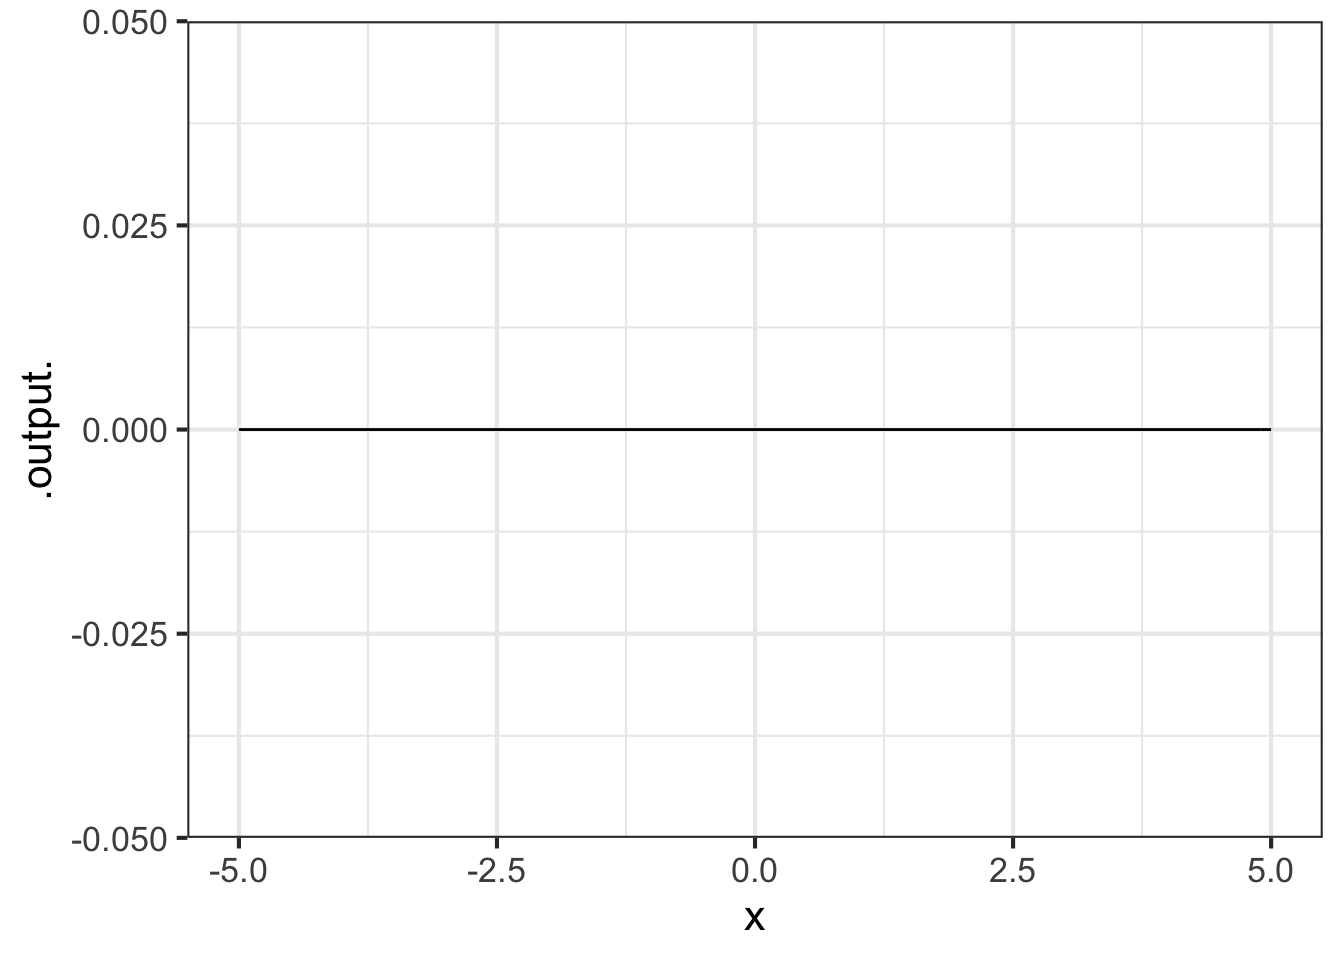
\includegraphics[width=0.9\textwidth,height=\textheight]{Accumulation/31-symbolic_files/figure-pdf/fig-check-constant-1.pdf}

}

\caption{\label{fig-check-constant}\textbf{?(caption)}}

\end{marginfigure}

\end{example}

\begin{example}
Task: Find \(\int \ln(x) dx\).

The easy solution is to recognize that the anti-derivative of \(\ln(x)\)
is contained in the table at the top of the chapter. But let's try doing
it by parts as an example (and to show you how it got into the table in
the first place).

It's hard to see a separate \(f(x)\) and \(g(x)\) in the integrand
\(\ln(x)\). But sometimes you need to be clever. We'll set
\(f(x) \equiv \ln(x)\) and \(g(x) \equiv 1\). This means that
\(G(x) = x\). The helper function is therefore \(h(x) = x\ln(x)\)

Differentiating the helper function gives (by the product rule):
\(\partial_x h(x) = \ln(x) + x \frac{1}{x} = \ln(x) + 1\)

Integrating the differentiated helper function, we find
\[\int \partial_x h(x) dx = f(x)g(x) = x \ln(x) = \underbrace{\int \ln(x) dx}_\text{The original integral} + \underbrace{\int 1 dx}_{x}\]
Re-arranging, we have
\[\underbrace{\int \ln(x) dx}_\text{The original integral} = x \ln(x) - x\ \  =\ \  x\left[\strut \ln(x) - 1\right]\]

\end{example}

\begin{example}
Task: Find \(\int \sin(x) e^x dx\).

This isn't the integral of a pattern book or basic modeling function,
and substitution didn't work, so we try integration by parts.

The obvious choice for the two parts is \(\sin(x)\) and \(e^x\). Both
are really easy to anti-differentiate. Let's choose \(g(x) = \sin(x)\),
giving \(G(x) = -\cos(x)\). The re-arrangement of the original integral
will be \[\sin(x) e^x + \int \cos(x) e^x dx\] The new integral that we
need to compute doesn't look any friendlier than the original, but who
knows? We'll do \(\int cos(x) e^x dx\) by parts as well and keep our
fingers crossed. That integral turns out to be
\[\int \cos(x) e^x dx = \cos(x) e^x - \int \sin(x) e^x dx\] This may
look like we're going in circles, and maybe we are, but let's put
everything together.
\[\underbrace{\int \sin(x) e^x dx}_\text{The original problem} = \underbrace{\sin(x) e^x + \cos(x) e^x}_\text{Easy stuff!}\ \ \  - \underbrace{\int \sin(x) e^x dx}_\text{Also the original problem}\]
Rearranging gives
\[\int \sin(x) e^x dx = \frac{\sin(x) e^x + \cos(x) e^x}{2} = \frac{e^x}{2}\left[{\large\strut} \sin(x) + \cos(x)\right]\]
And don't forget the constant of integration.

\end{example}

{[}The presentation of integration by parts in this section was
formulated by Prof.~Michael Brilleslyper.{]}

\hypertarget{didnt-work}{%
\section{Didn't work?}\label{didnt-work}}

If integration by parts doesn't work \ldots{} and it doesn't always
work! \ldots{} there is a variety of possibilities such as asking a math
professor (who has a much larger set of functions at hand than you),
looking through a table of integrals (which is to say, the collective
calculus diary of generations of math professors), using a computer
algebra system, or using numerical integration. One of these will work.

If you have difficulty using u-substitution or integration by parts, you
will be in the same league as the vast majority of calculus students.
Think of your fellow students who master the topic in the way you think
of ice dancers. It's beautiful to watch, but you need a special talent
and it hardly solves every problem. People who would fall on their face
if strapped to a pair of skates have nonetheless made huge contributions
in technical fields, even those that involve ice.

Prof.~Kaplan once had a heart-to-heart with a 2009 Nobel-prize winner
who confessed to always feeling bad and inadequate as a scientist
because he had not done well in introductory calculus. It was only when
he was nominated for the Nobel that he felt comfortable admitting to his
``failure.'' Even if you don't master u-substitution or integration by
parts, remember that you can integrate any function using easily
accessible resources.

\hypertarget{integrating-polynomials}{%
\section{Integrating polynomials}\label{integrating-polynomials}}

One of the most famous settings for integration comes from the physics
of free fall under gravity.

Here's the setting. An object---a ball, let's imagine---is being held at
height \(x_0\). At \(t=0\) the ball is released. Perhaps the ball is
released from a standstill in which case it's velocity at release is
\(v_0 = v(t=0) =0\). Or perhaps the ball has been tossed upward so that
\(v_0 > 0\), or downward so that \(v_0 < 0\). Whichever it is, the
initial velocity will be labelled \(v_0\).

On release, the force that held the ball steady is removed and the
object moves under the influence of only one factor: gravity. The effect
of gravity near the Earth's surface is easy to describe: it accelerates
the object at a constant rate of about 9.8 m/s\(^2\).

Acceleration is the derivative with respect to time of velocity. Since
we know acceleration, to find velocity we find an anti-derivative of
acceleration: \[v(t) = \int -9.8\ dt = -9.8\ t + C\] The constant of
integration \(C\) is not just a formality. It has physical meaning. In
this case, we see that \(C=v(0)\), that is, \(C = v_0\).

Velocity is the derivative of position: height in this case. So height
is an anti-derivative of velocity.
\[x(t) = \int v(t) dt = \int \left[\strut -9.8\ t + v_0\right]dt = - \frac{9.8}{2} t^2 + v_0\ t + C\]
Why is \(C\) back again? It's a convention to use \(C\) to denote the
constant of integration. Those experienced with this convention know,
from context, that the value of \(C\) in the integration that produced
\(v(t)\) has nothing to do with the value of \(C\) involved in the
production of \(x(t)\). The situation is a bit like the presentation of
prices in US stores: to the price of the item itself, you must always
add ``plus taxes.'' Nobody with experience would assume that ``taxes''
is always the same number. It depends on the price and type of the item
itself.\sidenote{\footnotesize Many jurisdictions tax food and clothing, etc. at a
  different rate than other items.} You won't have to deal with the
taxes at the time you pick the item from the shelf, but eventually
you'll see them when you check out of the store. Think of \(+\ C\) as
meaning, ``plus some number that we'll have to deal with at some point,
but not until checkout.''

Let's checkout the function \(x(t)\) now. For that, we need to figure
out the value of \(C\). We can do that by noticing that \(x(0) = C\). So
in the anti-differentiation producing \(x()\), \(C = x_0\) giving,
altogether the formula for free-fall famous from physics classes
\[x(t) =  - \frac{9.8}{2} t^2 + v_0\ t + x_0\] An important thing to
notice about \(x(t)\): it's a polynomial in \(t\). Polynomials can be
birthed by successive anti-differentiations of a constant. At each
anti-differentiation, each of the previous terms is promoted by one
order. That is, the previous constant becomes the first order term. The
previous first-order term becomes the second order term, with the
division by 2 familiar from anti-differentiating \(t\). A previous
second-order term will become the new third-order term, again with the
division by 3 familiar from anti-differentiating \(t^2\).

Stated generally, the anti-derivative of a polynomial is

\[{\Large\int} \left[\strut \underbrace{a + b t + ct^2 + \ldots}_\text{original polynomial}\right] dt = \underbrace{C + a\,t + \frac{b}{2} t^2 + \frac{c}{3} t^3 + \ldots}_\text{new polynomial}\]
By use of the symbol \(C\), it's easy to spot how the constant of
integration fits in with the new polynomial. But if we were to
anti-differentiate the new polynomial, we had better replace \(C\) with
some more specific symbol to that we don't confuse the old \(C\) with
the one that's going to be produced in the new anti-differentiation.

\begin{intheworld}
In exercise 26.16, we introduced a Taylor polynomial approximation to
the gaussian function. That might have seemed like a mere exercise in
high-order differentiation at the time, but there is something more
important at work.

The gaussian is one of those functions for which the anti-derivative
cannot be written exactly in terms of what the mathematicians call
``elementary functions.'' (See Section~\ref{sec-cataloged-functions}.)
Yet integrals of the gaussian are very commonly used in science,
especially in statistics where the gaussian is called the
\textbf{\emph{normal PDF}}.

The approach we've taken in this book is simply to give a name and a
computer implementation of the anti-derivative of the gaussian. This is
the function we've called \(\pnorm()\) with the R computer
implementation \texttt{pnorm()}.

We never told you the algorithm contained in \texttt{pnorm()}. Nor do we
really need to. We all depend on experts and specialists to design and
build the computers we use. The same is true of software implementation
of functions like \texttt{pnorm()}. And for that matter, for
implementations of functions like \texttt{exp()}, \texttt{log()},
\texttt{sin()}, and so on. You don't have to know about semi-conductors
in order to use a computer productively, and you don't need to know
about numerical algorithms in order to use those functions.

One feasible algorithm for implementing \(\pnorm()\) is to integrate the
Taylor polynomial. It's very easy integrate polynomials. To ensure
accuracy, different Taylor polynomials can be computed for different
centers, say \(x=0\), \(x=1\), \(x=2\), and so on.

Another feasible approach integrates \(\dnorm()\) numerically using an
advanced algorithm such as Gauss-Hermite quadrature.

\end{intheworld}

\hypertarget{exercises-4}{%
\section{Exercises}\label{exercises-4}}

\end{document}
